% This is "sig-alternate.tex" V2.1 April 2013
% This file should be compiled with V2.5 of "sig-alternate.cls" May 2012
%
% This example file demonstrates the use of the 'sig-alternate.cls'
% V2.5 LaTeX2e document class file. It is for those submitting
% articles to ACM Conference Proceedings WHO DO NOT WISH TO
% STRICTLY ADHERE TO THE SIGS (PUBS-BOARD-ENDORSED) STYLE.
% The 'sig-alternate.cls' file will produce a similar-looking,
% albeit, 'tighter' paper resulting in, invariably, fewer pages.
%
% ----------------------------------------------------------------------------------------------------------------
% This .tex file (and associated .cls V2.5) produces:
%       1) The Permission Statement
%       2) The Conference (location) Info information
%       3) The Copyright Line with ACM data
%       4) NO page numbers
%
% as against the acm_proc_article-sp.cls file which
% DOES NOT produce 1) thru' 3) above.
%
% Using 'sig-alternate.cls' you have control, however, from within
% the source .tex file, over both the CopyrightYear
% (defaulted to 200X) and the ACM Copyright Data
% (defaulted to X-XXXXX-XX-X/XX/XX).
% e.g.
% \CopyrightYear{2007} will cause 2007 to appear in the copyright line.
% \crdata{0-12345-67-8/90/12} will cause 0-12345-67-8/90/12 to appear in the copyright line.
%
% ---------------------------------------------------------------------------------------------------------------
% This .tex source is an example which *does* use
% the .bib file (from which the .bbl file % is produced).
% REMEMBER HOWEVER: After having produced the .bbl file,
% and prior to final submission, you *NEED* to 'insert'
% your .bbl file into your source .tex file so as to provide
% ONE 'self-contained' source file.
%
% ================= IF YOU HAVE QUESTIONS =======================
% Questions regarding the SIGS styles, SIGS policies and
% procedures, Conferences etc. should be sent to
% Adrienne Griscti (griscti@acm.org)
%
% Technical questions _only_ to
% Gerald Murray (murray@hq.acm.org)
% ===============================================================
%
% For tracking purposes - this is V2.0 - May 2012

\documentclass[acmsmall]{acmart}
%\documentclass[prodmode,acmtecs]{acmart}
\usepackage{balance}  % for  \balance command ON LAST PAGE  (only there!)
\usepackage{algorithm}
\usepackage{epsfig}
\usepackage{graphicx}
\usepackage{esvect} % for arrows
\usepackage{xspace,multirow,amsmath, color,array,colortbl} %
\usepackage{subfigure}
\usepackage[english]{babel}
\usepackage[bigsqcap]{stmaryrd}
%\usepackage{ulem}
%\usepackage{lmodern} %do not use lmodern, otherwise, brackets in equation will be lost.
%\usepackage{cite}

\newcommand{\imp}{\vdash_{\cal I}}


%%%%%%%%%%%%%%%%%%%%%%%%%%%%%%%%%%%%%%%%%%
% Enumerate and Itemize modifications
%\usepackage{enumitem}
%\setlist{topsep=0pt,noitemsep} \setitemize[1]{label=$\circ$}
%%%%%%%%%%%%%%%%%%%%%%%%%%%%%%%%%%%%%%%%%%%

\sloppy
\newcommand{\rtable}[1]{\ensuremath{\mathsf{#1}}}
\newcommand{\ratt}[1]{\ensuremath{\mathit{#1}}}
\newcommand{\at}[1]{\protect\ensuremath{\mathsf{#1}}\xspace}
\newcommand{\myhrule}{\rule[.5pt]{\hsize}{.5pt}}
\newcommand{\oneurl}[1]{\texttt{#1}}
\newcommand{\eat}[1]{}
\newcommand{\stab}{\rule{0pt}{8pt}\\[-1.6ex]}
\newcommand{\sttab}{\rule{0pt}{8pt}\\[-2ex]}
%\newcommand{\sstab}{\rule{0pt}{8pt}\\[-2.4ex]}
\newcommand{\tabstrut}{\rule{0pt}{4pt}\vspace{-0.07in}}
\newcommand{\vs}{\vspace{1ex}}
\newcommand{\exa}[2]{{\tt\begin{tabbing}\hspace{#1}\=\+\kill #2\end{tabbing}}}
\newcommand{\ra}{\rightarrow}
\newcommand{\la}{\leftarrow}
\newcommand{\bi}{\begin{itemize}}
\newcommand{\ei}{\end{itemize}}
\newenvironment{tbi}{\begin{itemize}
        \setlength{\topsep}{1.5ex}\setlength{\itemsep}{0ex}\vspace{-0.5ex}}
        {\end{itemize}\vspace{-0.5ex}}
\newenvironment{tbe}{\begin{enumerate}
        \setlength{\topsep}{0ex}\setlength{\itemsep}{-0.7ex}\vspace{-1ex}}
        {\end{itemize}\vspace{-1ex}}

\newcommand{\mat}[2]{{\begin{tabbing}\hspace{#1}\=\+\kill #2\end{tabbing}}}
\newcommand{\m}{\hspace{0.05in}}
\newcommand{\ls}{\hspace{0.1in}}
\newcommand{\be}{\begin{enumerate}}
\newcommand{\ee}{\end{enumerate}}
\newcommand{\beqn}{\begin{eqnarray*}}
\newcommand{\eeqn}{\end{eqnarray*}}
\newcommand{\card}[1]{\mid\! #1\!\mid}
\newcommand{\fth}{\hfill $\Box$}
\newcommand{\AND}{\displaystyle{\bigwedge_{i=1}^{n}}}
%\newcommand{\U}[1]{\displaystyle{\bigcup_{#1}}}
\newcommand{\Sm}[1]{\displaystyle{\sum_{#1}}}
\newcommand{\stitle}[1]{\vspace{1ex}\noindent{\bf #1}}
\newcommand{\etitle}[1]{\vspace{0.5ex}\noindent{\em \underline{#1}}}
\renewcommand{\t}{\tau}
\newcommand{\Inh}[1]{\$#1}
\renewcommand{\r}[1]{{\it rule}(#1)}
\newcommand{\pa}{\parallel}
\newcommand{\LHS}{\kw{{\small LHS}}}
\newcommand{\RHS}{\kw{RHS}}
\newcommand{\len}{\kw{len}}
\newcommand{\kop}{\kw{op}}
%\newcommand{\st}{\emph{s.t.}\xspace}
\newcommand{\ie}{\emph{i.e.,}\xspace}
\newcommand{\eg}{\emph{e.g.,}\xspace}
\newcommand{\wrt}{\emph{w.r.t.}\xspace}
\newcommand{\aka}{\emph{a.k.a.}\xspace}
\newcommand{\kwlog}{\emph{w.l.o.g.}\xspace}

\newcommand{\VNM}{\kw{VNM}}
\newcommand{\VNMs}{\kw{VNM}}
\newcommand{\VN}{\kw{VN}}
\newcommand{\SN}{\kw{SN}}

%%%%%%%%%%%%%%%%%%%%%%%%%%%%%%%%%%%%%%%%%%%%%%%%%%%%%%%%%%%%%%%%
%                  Relation Algebra operators
%%%%%%%%%%%%%%%%%%%%%%%%%%%%%%%%%%%%%%%%%%%%%%%%%%%%%%%%%%%%%%%%

\newcommand{\RS}{{\small S}\xspace}
\newcommand{\RP}{{\small P}\xspace}
\newcommand{\RJ}{{\sc j}\xspace}
\newcommand{\RC}{{\small C}\xspace}
\newcommand{\RSJ}{{\small SJ}\xspace}
\newcommand{\RSC}{{\small SC}\xspace}
\newcommand{\RSP}{{\small SP}\xspace}
\newcommand{\RPJ}{{\small PJ}\xspace}
\newcommand{\RPC}{{\small PC}\xspace}
\newcommand{\RSPJ}{{\sc spj}\xspace}
\newcommand{\RSPC}{{\small SPC}\xspace}
\newcommand{\RSPJU}{{\sc spju}\xspace}
\newcommand{\RSPCU}{{\small SPCU}\xspace}
\newcommand{\RSPJUN}{{\small SPJU$^N$}\xspace}
\newcommand{\RSPCUN}{{\small SPCU$^N$}\xspace}
%%%%%%%%%%%%%%%%%%%%%%%%%%%%%%%%%%%%%%%%%%%%%%%%%%%%%%%%%%%%%%%%%%%%%%%%%%%%%%
% ALGORITHMS
%%%%%%%%%%%%%%%%%%%%%%%%%%%%%%%%%%%%%%%%%%%%%%%%%%%%%%%%%%%%%%%%%%%%%%%%%%%%%%%

\newcommand{\kw}[1]{{\ensuremath {\mathsf{#1}}}\xspace}

\newcounter{ccc}
\newcommand{\bcc}{\setcounter{ccc}{1}\theccc.}
\newcommand{\icc}{\addtocounter{ccc}{1}\theccc.}
\newcommand{\checking}{{\mbox{\small\sf Checking}\xspace}}
\newcommand{\preProcessing}{{\mbox{\small\sf preProcessing}\xspace}}
\newcommand{\CFDconsistency}{{\mbox{\small\sf CFD\_Checking}\xspace}}
\newcommand{\MCS} {\kw{MCS}}
\newcommand{\templateDB}{{\mbox{\small\sf templateDB}\xspace}}
\newcommand{\ChaseChecking}{{\mbox{\small\sf RandomChecking}\xspace}}
\newcommand{\chase}{{\mbox{\small\sf Chase}\xspace}}
\newcommand{\SAT}{{\mbox{\small\sf SAT}\xspace}}
\newcommand{\kSAT}{{\mbox{\small 3SAT}\xspace}}
\newcommand{\PropCFDSPC}{\kw{Prop{\small CFD\_SPC}}}
\newcommand{\PropCFDSPCU}{\kw{Prop{\small CFD\_SPCU}}}
\newcommand{\UnionEQs}{\kw{UnionEQs}}
\newcommand{\UnionCFDs}{\kw{UnionCFDs}}
\newcommand{\EQ}{\kw{EQ}}
\newcommand{\eq}{\kw{eq}}
\newcommand{\key}{\kw{key}}
\newcommand{\rep}{\kw{rep}}
\newcommand{\PEQ}{\kw{EQ2CFD}}
\newcommand{\Drop}{\kw{Drop}}
%\newcommand{\Res}{\kw{Res}}
\newcommand{\CFD}{{\small CFD}\xspace}
\newcommand{\CFDs}{{\small CFD}{\small s}\xspace}
\newcommand{\CIND}{{\sc cind}\xspace}
\newcommand{\cind}{{\small \sf CIND}}
\newcommand{\cfd}{{\small \sf CFD}}
\newcommand{\CINDp}{{\sc cind}$^+$\xspace}
\newcommand{\CINDn}{{\sc cind}$^-$\xspace}
\newcommand{\CINDs}{{\sc cind}{\small s}\xspace}
\newcommand{\FD}{{\small FD}\xspace}
\newcommand{\FDs}{{\small FD}{\small s}\xspace}
\newcommand{\IND}{{\sc ind}\xspace}
\newcommand{\INDs}{{\sc ind}{\small s}\xspace}
\newcommand{\TGDs}{{\sc tgd}{\small s}\xspace}
\newcommand{\NP}{{\small NP}\xspace}
\newcommand{\DTIME}{{\small DTIME}\xspace}
\newcommand{\NPO}{{\small NPO}\xspace}
\newcommand{\APX}{{\small APX}\xspace}
\newcommand{\DAGs}{{\sc dag}s\xspace}
\newcommand{\NC}{{\sc nc}\xspace}
\newcommand{\coNP}{co{\small NP}\xspace}
\newcommand{\PTIME}{{\small PTIME}\xspace}
\newcommand{\PSPACE}{{\sc pspace}\xspace}
\newcommand{\EXPTIME}{{\sc exptime}\xspace}
\newcommand{\NPSPACE}{{\sc npspace}\xspace}
\newcommand{\dom}{\protect\ensuremath{\mathsf{dom}}\xspace}
\newcommand{\atset}{\protect\ensuremath{\mathsf{attr}}\xspace}
\newcommand{\attr}[1]{\protect\ensuremath{\mathsf{#1}}\xspace}
\newcommand{\attrset}{\protect\ensuremath{\mathsf{attr}}\xspace}
\newcommand{\finatset}{\protect\ensuremath{\mathsf{finattr}}\xspace}
\newcommand{\pvar}{\protect\ensuremath{\mathsf{var\%}}\xspace}
\newcommand{\lLHS}{\protect\ensuremath{\mathsf{{\small LHS}}}\xspace}
\newcommand{\RA}{{\small RA}\xspace}
\newcommand{\RBR}{\kw{RBR}}
\newcommand{\SQL}{{\sc sql}\xspace}
\newcommand{\XSLT}{{\sc xslt}\xspace}
\newcommand{\DBMS}{{\sc dbms}\xspace}
\newcommand{\ATG}{{\sc atg}\xspace}
\newcommand{\ATGs}{{\sc atg}{\small s}\xspace}
\newcommand{\EBI}{{\sc ebi}\xspace}
\newcommand{\GO}{{\sc go}\xspace}
\newcommand{\VEC}[1]{{\sc vec}(#1)}
\newcommand{\DAG}{{\sc dag}\xspace}
\newcommand{\XQ}{{\sc xq}\xspace}
\newcommand{\XQwc}{{\sc xq}$^{\scriptscriptstyle[*]}$\xspace}
\newcommand{\XQdes}{{\sc xq}$^{\scriptscriptstyle[//]}$\xspace}
\newcommand{\XQfull}{{\sc xq}$^{\scriptscriptstyle[*,//]}$\xspace}
\newcommand{\vect}[1]{$\langle$ #1 $\rangle$}
\newcommand{\sem}[1]{[\![#1]\!]}
\newcommand{\NN}[2]{#1\sem{#2}}
\newcommand{\e}[2]{{\mathit (#1,#2)}}
\newcommand{\ep}[2]{{\mathit (#1,#2)+}}
\newcommand{\brname}{\ensuremath{{\mathsf{N}}}}
\newcommand{\budrel}[1]{\ensuremath{{\brname_{#1}}}}
\newcommand{\budgen}[2]{\ensuremath{Q^\brname_\e{#1}{#2}}}
\newcommand{\budcut}[2]{\ensuremath{Q_\e{#1}{#2}}}
\newcommand{\eop}{\hspace*{\fill}\mbox{$\Box$}}     % End of proof
\newcounter{example}%[section]
%\newcommand{\theexample}{\arabic{example}}
\newenvironment{example}{
         \vspace{1.5ex}
         \refstepcounter{example}
         {\noindent\bf Example \theexample:}}{
         \eop\vspace{1.5ex}}
\def\copyrightspace{}
\renewcommand{\ni}{\noindent}
\newcommand{\comlore}[1]{\begin{minipage}{3in}\fbox{\fbox{\parbox[t]{3in}{{\vspace{2mm}\noindent \bf COMM(LORE):~
{ #1}\hfill  END.}}}}\end{minipage}\\}
\newcommand{\comwenfei}[1]{\begin{minipage}{3in}\fbox{\fbox{\parbox[t]{3in}{{\vspace{2mm}\noindent \bf COMM(WENFEI):~
{ #1}\hfill  END.}}}}\end{minipage}\\}
\newcommand{\comshuai}[1]{\begin{minipage}{3in}\fbox{\fbox{\parbox[t]{3in}{{\vspace{2mm}\noindent \bf COMM(SHUAI):~
{ #1}\hfill  END.}}}}\end{minipage}\\}
\newcommand{\nthesection}{\arabic{section}}
%\newcounter{problem}
%\newenvironment{problem}{\begin{em}
%        \refstepcounter{problem}
%        {\vspace{1.5ex} \noindent\bf Problem \theproblem:}}{
%        \end{em}\eop\vspace{1.5ex}}
\newcounter{prop}[section]
%\renewcommand{\theprop}{\arabic{theorem}}
%\newcounter{lemma}[section]
%\renewcommand{\thelemma}{\arabic{theorem}}
%\newcounter{cor}[section]
%\renewcommand{\thecor}{\arabic{theorem}}
\newenvironment{ttheorem}{\begin{em}
         \refstepcounter{theorem}
         {\vspace{1.5ex} \noindent\bf  Theorem  \thetheorem:}}{
        \end{em}\eop\vspace{1.5ex}} %\hspace*{\fill}\vspace*{1ex}}
\newenvironment{pprop}{\begin{em}
        \refstepcounter{theorem}
        {\vspace{1.5ex}\noindent \bf Proposition \thetheorem:}}{
        \end{em}\eop\vspace{1.5ex}}%\hspace*{\fill}\vspace*{1ex}}
\newenvironment{llemma}{\begin{em}
         \refstepcounter{theorem}
        {\vspace{1.5ex}\noindent\bf Lemma \thetheorem:}}{
         \end{em}\eop\vspace{1.5ex}} %\hspace*{\fill}\vspace*{1ex}}
\newenvironment{cor}{\begin{em}
        \refstepcounter{theorem}
        {\vspace{1.5ex}\noindent\bf Corollary \thetheorem:}}{
        \end{em}\eop\vspace{1.5ex}} %\hspace*{\fill}\vspace*{1ex}}

%\newcounter{definition}
%\renewcommand{\thedefinition}{\arabic{definition}}
%\newenvironment{definition}{
%        \vspace{1.5ex}
%        \refstepcounter{definition}
%        {\noindent\bf Definition {\bf \thedefinition}:}}{\eop\vspace{1.5ex}
%}
\newcounter{alg}[section]
\renewcommand{\thealg}{\nthesection.\arabic{alg}}
\newenvironment{alg}[1]{
        \refstepcounter{alg}
        {\vspace{1ex}\noindent\bf Algorithm \thealg:\, #1}}{
        \vspace*{1ex}}
\newcounter{arule}
\renewcommand{\thearule}{\arabic{arule}}
\newenvironment{arule}{
        \vspace{0.6ex}
        \refstepcounter{arule}
        {\noindent \em Rule \thearule:}}{
        }
\newcounter{claim}
\renewcommand{\theclaim}{\arabic{claim}}
\newenvironment{claim}{
        \vspace{0.6ex}
        \refstepcounter{claim}
        {\noindent\em Claim \theclaim:}}{%--{ Wenfei Fan}\\
        }
\renewenvironment{proof}{
%\newenvironment{proof}{
        \vspace{0ex}
        {\noindent\bf Proof:}}{\eop\vspace{1ex}}
\newenvironment{proofS}{
        \vspace{1ex}
        {\noindent\bf Proof sketch:\ }}{\eop\vspace{1ex}}

\newcommand{\dist}{\kw{ldist}}
\newcommand{\pSim}{\kw{JoinMatch}}
\newcommand{\spSim}{\kw{SplitMatch}}
\newcommand{\gpq}{\kw{PQ}}
\newcommand{\gpqs}{\kw{PQs}}
\newcommand{\rrq}{\kw{RQ}}
\newcommand{\rrqs}{\kw{RQs}}
\newcommand{\rpe}{\kw{RPE}}
\newcommand{\rpes}{\kw{RPEs}}

\newcommand{\eps}{\trianglelefteq}
\newcommand{\neps}{\ntrianglelefteq}
\newcommand{\ees}{\preceq_{(e,e)}}
\newcommand{\nees}{\not\preceq_{e,e}}
\newcommand{\Reps}{S}

\newcommand{\added}[1]{\textcolor{blue}{#1}}
\newcommand{\changed}[1]{\textcolor{red}{#1}}
\newcommand{\removed}[1]{\textcolor{gray}{#1}}

\newcommand{\ret}{\kw{ret}}
\newcommand{\remv}{\kw{premv}}
\newcommand{\presim}{\kw{amat}}
\newcommand{\prev}{\kw{prev}}
\newcommand{\subiso}{\kw{SubIso}}

\newcommand{\ssim}{\kw{mat}}
\newcommand{\join}{\kw{Join}}
\newcommand{\nor}{\kw{Normalize}}
\renewcommand{\split}{\kw{Split}}
\newcommand{\sccg}{\kw{Sccgraph}}
\newcommand{\rmv}{\kw{rmv}}
\newcommand{\block}{{\cal B}}
\newcommand{\rel}{\kw{rel}}
\newcommand{\partition}{\kw{par}}
\newcommand{\cpath}{{\em c}-path\xspace}
\newcommand{\cpaths}{{\em c}-paths\xspace}
\newcommand{\psimset}{\kw{Psim}}



\newcommand{\vn}{\kw{VN}}
\newcommand{\vns}{\kw{VNs}}
\newcommand{\sns}{\kw{SNs}}
\newcommand{\vm}{\kw{VM}}
\newcommand{\vms}{\kw{VMs}}
\newcommand{\vmp}{\kw{VMP}}
\newcommand{\sn}{\kw{SN}}
\newcommand{\vne}{\kw{VNE}}

\newcommand{\buildAug}{\kw{compAuxGraph}}
\newcommand{\minVN}{\kw{minVN}}
\newcommand{\compMap}{\kw{compVNM}}
\newcommand{\compMapNS}{\kw{compVNM_{NS}}}
\newcommand{\PTAS}{{\small PTAS}\xspace}
\newcommand{\APTAS}{{\small APTAS}\xspace}
\newcommand{\VM}{\kw{VM}}
\newcommand{\vine}{\kw{ViNE}}
\newcommand{\vineNS}{\kw{ViNE_{NS}}}
\newcommand{\rwsp}{\kw{RW}-\kw{SP}}
\newcommand{\lvb}{\{\!|}
\newcommand{\rvb}{|\!\}}
%% APPENDIX

\newcommand{\gap}{\kw{GAP}}
\newcommand{\rgap}{\kw{RGAP}}
\newcommand{\subgIso}{\kw{Subgraph} \kw{Isomorphism}}
\newcommand{\xtc}{\kw{X3C}}
\newcommand{\binpack}{\kw{Bin} \kw{Packing}}
\newcommand{\parti}{\kw{PARTITION}}
\newcommand{\mwsat}{\kw{Minimum} \kw{Weight} \kw{3SAT}}
\newcommand{\edp}{\kw{EDP}}
\newcommand{\att}{\SIM}
\newcommand{\swsf}{\kw{SWSF\_FP}}

\newcommand{\warn}[1]{\textcolor{red}{#1}}
\newcommand{\revise}[1]{\textcolor{blue}{#1}}
\newcommand{\marked}[1]{\revise{#1}}


%%%%%%%%%%%%%%%%%%%%%%%%%%%%%%%%%%%%%%%%%%%%%%%%%%%%%%%%%%
\newcommand{\lsa}{\kw{LS}}
\newcommand{\dpa}{\kw{DP}}
\newcommand{\dpp}{\kw{DPPED}}
\newcommand{\dps}{\kw{DPSED}}
\newcommand{\dpsed}{\kw{DPSED}}


\newcommand{\opwa}{\kw{OPW}}
\newcommand{\bqsa}{\kw{BQS}}
\newcommand{\fbqsa}{\kw{FBQS}}
\newcommand{\operb}{\kw{OPERB}}
\newcommand{\operba}{\kw{OPERB}-\kw{A}}
\newcommand{\squish}{\kw{SQUISH}}
\newcommand{\squishe}{\kw{SQUISH}-\kw{E}}
\newcommand{\siped}{\kw{SIPED}}
\newcommand{\sleeve}{\kw{Sleeve}}
\newcommand{\conei}{\kw{Cone~Intersection}}
\newcommand{\cised}{\kw{CISED}}
\newcommand{\ridad}{\kw{RIDAD}}
%\newcommand{\intersec}{\kw{RangeIS}}
\newcommand{\intersec}{\kw{Intersect}}
\newcommand{\interval}{\kw{Interval}}

\newcommand{\douglas}{\kw{Douglas}-\kw{Peucker}}
\newcommand{\pavlidis}{\kw{Theo}-\kw{Pavlidis}}
\newcommand{\tpa}{\kw{TP}}
\newcommand{\reumann}{\kw{Reumann}-\kw{Witkam}}
\newcommand{\rwa}{\kw{RW}}
\newcommand{\ldr}{\kw{LDR}} %Linear Dead Reckoning
\newcommand{\swab}{\kw{SWAB}}

\newcommand{\opt}{\kw{Optimal}}
%\newcommand{\opt}{\kw{NaiveOpt}}
\newcommand{\optp}{\kw{OptPED}}
%\newcommand{\opts}{\kw{OptSED}}
%\newcommand{\nopts}{\kw{NearOptSED}}

%%%%%%%%%%%%%%%%%%%%%%%%%%%%%%%Data sets%%%%%%%%%%%%%%%%%
\newcommand{\taxi}{\kw{Taxi}}
\newcommand{\truck}{\kw{Truck}}
%\newcommand{\serviceCar}{\kw{UCar}}
%\newcommand{\pricar}{\kw{PrivateCar}}
\newcommand{\ucar}{\kw{UCar}}
\newcommand{\geolife}{\kw{Geolife}}
\newcommand{\mopsi}{\kw{Mopsi}}
%\newcommand{\act}{\kw{Act}}
%\newcommand{\dSets}{(\taxi, \ucar, \geolife, \mopsi)}
\newcommand{\dSets}{(\ucar, \geolife, \mopsi)}


\newcommand{\trajec}[1]{$\dddot{\mathcal{#1}}$}
\newcommand{\ffunc}[1]{{\mathbb{#1}}}
\newcommand{\anoline}{\kw{AL}}


%%%%%%%%%%%%%%%%%%%%%%%%%%%%%%DualError%%%%%%%%%%%%%%%%%%
\newcommand{\ped}{\kw{PED}} %perpendicular Euclidean distance (PED).
\newcommand{\sed}{\kw{SED}} %synchronous Euclidean distance (SED).
\newcommand{\dad}{\kw{DAD}} %Direction-Aware Distance (DAD).



%\newcommand{\red}{\kw{RED}} %radial Euclidean distance (RED).
%\newcommand{\ded}{\kw{DED}} %dual Euclidean distance (DED).


\newcommand{\sector}[1]{{$\mathcal{S}{#1}$}}
\newcommand{\cone}[1]{{$\mathcal{C}{#1}$}}
\renewcommand{\circle}[1]{{$\mathcal{O}{#1}$}}
\newcommand{\pcircle}[1]{{$\mathcal{O}^c{#1}$}}

%\newcommand{\mytable}[1]{\fcolorbox{red}{white}{Table~\ref{#1}}}
\newcommand{\mytable}[1]{\textcolor{blue}{Table~\ref{#1}}}
\newcommand{\myfig}[1]{\fcolorbox{red}{white}{Figure~\ref{#1}}}

\newcommand{\todo}[1]{\textcolor{red}{Todo...#1}}

% Copyright
%\setcopyright{acmcopyright}
%\setcopyright{acmlicensed}
%\setcopyright{rightsretained}
%\setcopyright{usgov}
%\setcopyright{usgovmixed}
%\setcopyright{cagov}
%\setcopyright{cagovmixed}

%% DOI
%\doi{10.475/123_4}

%% ISBN
%\isbn{123-4567-24-567/08/06}

%%Conference
%\conferenceinfo{PLDI '13}{June 16--19, 2013, Seattle, WA, USA}

%\acmPrice{\$15.00}

%\conferenceinfo{VLDB}{'18, Munich, Germany}
%\CopyrightYear{2017} % Allows default copyright year (20XX) to be over-ridden - IF NEED BE.
%\crdata{0-12345-67-8/90/01}  % Allows default copyright data (0-89791-88-6/97/05) to be over-ridden - IF NEED BE.
%\setcopyright{acmcopyright}
% --- End of Author Metadata -----





\begin{document}

%\title{Trajectory Compression and Line Simplification: An Experimental Evaluation}
%\title{Linear Approximation of Trajectory: An Experimental Evaluation}
%\title{Line Simplification Algorithms for Trajectory Compression: A Comprehensive Evaluation and Experimental Study}
\title{Error Bounded Line Simplification Algorithms for Trajectory Compression: An Experimental Evaluation}

%\titlenote{A full version of this paper is available as
%\textit{Author's Guide to Preparing ACM SIG Proceedings Using
%\LaTeX$2_\epsilon$\ and BibTeX} at
%\texttt{www.acm.org/eaddress.htm}}}
%
% You need the command \numberofauthors to handle the 'placement
% and alignment' of the authors beneath the title.
%
% For aesthetic reasons, we recommend 'three authors at a time'
% i.e. three 'name/affiliation blocks' be placed beneath the title.
%
% NOTE: You are NOT restricted in how many 'rows' of
% "name/affiliations" may appear. We just ask that you restrict
% the number of 'columns' to three.
%
% Because of the available 'opening page real-estate'
% we ask you to refrain from putting more than six authors
% (two rows with three columns) beneath the article title.
% More than six makes the first-page appear very cluttered indeed.
%
% Use the \alignauthor commands to handle the names
% and affiliations for an 'aesthetic maximum' of six authors.
% Add names, affiliations, addresses for
% the seventh etc. author(s) as the argument for the
% \additionalauthors command.
% These 'additional authors' will be output/set for you
% without further effort on your part as the last section in
% the body of your article BEFORE References or any Appendices.


%\numberofauthors{1} %  in this sample file, there are a *total*

%%%%%%%%%%%%%%%%%%%%%%%%%%%%%%%%%%%%%%%%%%%%%%%%%%%%%%%%%%%%%%%%%%
%\author{
%\alignauthor
%    Xuelian Lin\hspace{1.5ex} Shuai Ma$^{*}$\hspace{1.5ex}  Jiahao Jiang\hspace{1.5ex}  Yanchen Hou\hspace{1.5ex} Tianyu Wo\hspace{1.5ex}\\
%    \affaddr{Beijing Advanced Innovation Center for Big Data and Brain Computing, Beijing, China}\\
%    \affaddr{SKLSDE Lab, Beihang University, Beijing, China}\\
%     \email{\{linxl, mashuai, jiangjh,  houyc, woty\}@buaa.edu.cn}  %, hucm, woty
%}
\author{Anonymous}
%%%%%%%%%%%%%%%%%%%%%%%%%%%%%%%%%%%%%%%%%%%%%%%%%%%%%%%%%%%%%%%%%%%

\begin{abstract}
Nowadays, various sensors are collecting, storing and transmitting tremendous trajectory data, and it is well-known that the storage, network bandwidth and computing resources could be heavily wasted if raw trajectory data is directly adopted. Line simplification algorithms are effective approaches to attacking this issue by compressing data points in a trajectory to a set of continuous line segments, and are commonly used in practice.
In this article,  we first classify the error bounded line simplification algorithms into different categories, and review each category of algorithms. We then study the data aging problem of line simplification  algorithms and distance metrics from the views of aging friendliness and aging error, and provide a full picture of the data aging problem. Finally, we present a systematic experimental evaluation of representative error bounded line simplification algorithms, including both optimal and sub-optimal methods, in terms of commonly adopted perpendicular Euclidean, synchronous Euclidean and direction-aware distances.
Using real-life trajectory datasets, we systematically evaluate and analyze the performance (compression ratio, average error, running time, {aging friendliness and query friendliness}) of error bounded line simplification algorithms with respect to {distance metrics,} trajectory sizes and error bounds.
Our study reveals the characteristics of error bounded line simplification algorithms, which lead to guidelines for practitioners to choose appropriate algorithms and distance metrics for specific applications.
\end{abstract}


\maketitle

%%%%%%%%%%%%%%%%%%%%%%%%%%%%%%%Region Start%%%%%%%%%%%%%%%%%%%%%%%%%%%%%%%%%
% The code below should be generated by the tool at
% http://dl.acm.org/ccs.cfm
% Please copy and paste the code instead of the example below.
%


%
% End generated code
%%%%%%%%%%%%%%%%%%%%%%%%%%%%%%%Region End%%%%%%%%%%%%%%%%%%%%%%%%%%%%%%%%%

%
%  Use this command to print the description
%
%\printccsdesc

% We no longer use \terms command
%\terms{Theory}

%\keywords{trajectory compression; line simplification}


%%% Local Variables:
%%% mode: latex
%%% TeX-master: "gis18"
%%% End:

\section{introduction}
\label{sec-intro}


\textit{Trajectory tracking} \cite{Lange:Tracking} is a combination of \textit{position tracking} \cite{Wolfson:PositionTracking,Leonhardi:Comparison} and \textit{trajectory simplification} \cite{Lin:Cised,Zhang:Evaluation} in one routine, where \textit{position tracking} is an approach that lets the moving objects database (MOD) server know the current position of a moving object effectively and efficiently, that is, it achieves the desired accuracy of the location information on the server by transmitting as few messages as possible \cite{Leonhardi:Comparison}. Linear dead reckoning (\ldr) \cite{Wolfson:PositionTracking} is such a widely used position tracking method, which is essentially an agreement between a given moving object and a MOD server such that the server could infer the current, excepted position of the moving object whose distance to the actual position of the object is bounded by a user specified threshold;
%
and \textit{trajectory simplification} \cite{Lin:Cised,Zhang:Evaluation} is to approximate a fine trajectory with a coarse one (whose corresponding data points are a subset of the original one), such that the size of the trajectory is reduced under a constrain that the maximum distance of the former to the latter is bounded by a user specified threshold. 
%Linear simplification \cite{Lin:Cised,Zhang:Evaluation} is such an effective and efficient approach that is also widely used in practice.
%
Position tracking and trajectory simplification both are the fundamental technologies of trajectory management and they also share some common target and strategy, \ie, reduce the number of messages or the size of trajectory data by discarding some location information that seems not that important, hence, researchers are trying to combine them in one routine and make it be suitable to run in resource constraint devices.

The authors of \cite{Trajcevski:LDRH} find that the position tracking algorithm \ldr with some tiny modifications is applicable to both track the positions of a moving object and simplify the trajectory built out of these positions. The modified \ldr,  called \ldrh in \cite{Lange:Tracking}, is the first trajectory tracking algorithm that combines position tracking and trajectory simplification into one consistent process. It is concise and efficient, and is suitable for mobile devices. However, it suffers in effectiveness in terms of compression ratio and communication cost, due to the nature of \ldr. 
%
Then, a framework, named the generic remote trajectory simplification (GRTS) \cite{Lange:GRTS,Lange:Tracking}, is developed to improve the effectiveness of trajectory tracking by separate position tracking and trajectory simplification into two sub-processes, where the positions of a moving object is also tracked by \ldr, and these positions are temporarily saved in a buffer and then simplified by some third-party line simplification algorithm. Indeed, it is more effective than \ldrh at a cost of weakening the conciseness and efficiency of \ldrh.
%



\stitle{\todo{Motivations}.}

\ni(1) Trajectory track algorithms are supposed to run in resource-constraint mobile devices, thus, besides good performance of efficiency and effectiveness, they should also be simple and light, \ie having low time and space complexities, otherwise, they are not suitable to run in those mobile devices. In response to these requirements, \ldrh is light, simple and efficient, but not effective; and \grts is effective, but not efficient and light enough. That is, neither of them is the ideal solution for trajectory tracking.
%The emerging of one pass trajectory simplification algorithms. These algorithms can be integrated into grts, however, it is not a natural way to implement a one-pass trajectory tracking algorithm like this way. Acutually, one pass position tracking + one pass trajectory simplification = one pass and effective trajectory tracking algorithm......co-design, like LDRH, yet more effective.


\ni(2) The current works, \ie~\ldrh and \grts, only compress a trajectory or track a moving object in circular areas, \ie the moving object is supposed to locate in a circular taking the expected position of the object as the center. However, in practical, there is a need to track moving objects in other areas, such as strip or rectangular-like areas. \todo{examples and figures of areas,}





\stitle{\todo{Contributions}.}
To the end, we design ways for trajectory tracking in varied areas, including strip and combined areas, and provide three novel one-pass algorithms tracking moving objects effectively and efficiently. 

1. one-pass tracking moving object in circular, citt, effectively and efficiently.

2. one-pass tracking in strips using ped. sitt.
a way that customize region by sed and ped. and implement it in position tracking LDR and trajectory tracking framework GRTS. advantage...

3. one-pass tracking in combined areas using sed and ped. bitt.  
A one-pass trajectory tracking algorithm supporting sed and ped, by a combination cone intersection and sector intersection, \ie co-design of position tracking and trajectory simplification, effective and low time and space complexity, suitable running in resource constraint devices.

4. experiments

\stitle{{Organization}}.
The remainder of the paper is organized as follows:
Section \ref{sec-pre} introduces the basic concepts and the basic HMM method,
Section \ref{sec-method} presents our trajectory simplification aware map-matching method,
Section \ref{sec-exp} reports the experimental results of these methods, followed by related works in Section \ref{sec-related} and conclusion in Section \ref{sec-conclusion}.




\section{Preliminaries}
In this section, we introduce basic concepts and cone intersection based one-pass algorithms using the perpendicular Euclidean distances for trajectory compression.
%\textcolor[rgb]{1.00,0.00,0.00}{A discussion and summary is presented in the last.}


%%%%%%%%%%%%%%%%%%%%%%%%%%%%%%%%%%%%%%%%%%%%%%%%%%%%%%%%%
% Cone Intersection
%%%%%%%%%%%%%%%%%%%%%%%%%%%%%%%%%%%%%%%%%%%%%%%%%%%%%%%%%
\begin{figure*}[tb!]
\centering
\includegraphics[scale=0.8]{figures/Fig-sleeve.png}
\vspace{-2.5ex}
\caption{\small The trajectory $\dddot{\mathcal{T}}[P_0, \ldots, P_{10}]$ is compressed by the \conei algorithm to two line segments.}
\vspace{-2ex}
\label{fig:sleeve}
\end{figure*}



\subsection{Basic Notations}

We first introduce basic notations.

\stitle{Points ($P$)}. A data point is defined as a triple $P(x, y, t)$, which represents that a moving object is located at {\em longitude} $x$ and {\em latitude} $y$ at {\em time} $t$. Note that data points can be viewed as points in a three-dimension Euclidean space.

\stitle{Trajectories ($\dddot{\mathcal{T}}$)}. A trajectory $\dddot{\mathcal{T}}[P_0, \ldots, P_n]$ is a sequence of data points in a monotonically increasing order of their associated time values (\ie $P_i.t < P_j.t$ for any $0\le i<j\le n$). Intuitively, a trajectory is the path (or track) that a moving object follows through space as a function of time~\cite{physics-trajectory}.


\stitle{Directed line segments ($\mathcal{L}$)}. A directed line segment (or line segment for simplicity) $\mathcal{L}$ is defined as $\vv{P_{s}P_{e}}$, which represents the closed line segment that connects the start point $P_s$ and the end point $P_e$.
Note that here $P_s$ or $P_e$ may not be a point in a trajectory $\dddot{\mathcal{T}}$, and hence, we also use notation $\mathcal{R}$ instead of $\mathcal{L}$ when both $P_s$ and $P_e$ belong to $\dddot{\mathcal{T}}$.

We also use $|\mathcal{L}|$ and $\mathcal{L}.\theta\in [0, 2\pi)$ to denote the length of a directed line segment $\mathcal{L}$, and its angle with the $x$-axis of the coordinate system $(x, y)$, where $x$ and $y$ are the longitude and latitude, respectively.
That is, a directed line segment $\mathcal{L}$ = $\vv{P_{s}P_{e}}$ can be treated as a triple $(P_s, |\mathcal{L}|, \mathcal{L}.\theta)$.

\stitle{Piecewise line representation ($\overline{\mathcal{T}}$)}. A piece-wise line representation of a trajectory $\dddot{\mathcal{T}}[P_0, \ldots, P_n]$ is denoted as $\overline{\mathcal{T}}[\mathcal{L}_0, \ldots , \mathcal{L}_m]$ ($0< m \le n$), a sequence of continuous directed line segments $\mathcal{L}_{i}$ = $\vv{P_{s_i}P_{e_i}}$ of $\dddot{\mathcal{T}}$ ($i\in[0,m]$)  such that $\mathcal{L}_{0}.P_{s_0} = P_0$, $\mathcal{L}_{m}.P_{e_m} = P_n$ and  $\mathcal{L}_{i}.P_{e_i}$ = $\mathcal{L}_{i+1}.P_{s_{i+1}}$ for all $i\in[0, m-1]$. Note that each directed line segment in $\overline{\mathcal{T}}$ essentially represents a continuous sequence of data points in $\dddot{\mathcal{T}}$.

%%%%%%%%%%%%%%%%%%%%%%%%%%%%%%%%%%%%%%%%%%%%%%%%%%%%%%%%%%%%%%%%%%%%%%%%%%%%%%
\eat{
\subsubsection{Notations of error metrics}

{For line simplification, there are distance based and shape based error metrics\cite{Shi:Survey} that measure the errors between the original trajectory and the simplified trajectory.
However, for trajectory simplification, the distance based metrics are definitely the distinct metrics.}

\stitle{Included angles ($\angle$)}. Given two directed line segments $\mathcal{L}_1$ = $\vv{P_{s}P_{e_1}}$ and $\mathcal{L}_2$ = $\vv{P_{s}P_{e_2}}$ with the same start point $P_s$, the included angle from $\mathcal{L}_1$ to $\mathcal{L}_2$, denoted as $\angle(\mathcal{L}_1, \mathcal{L}_2)$,  is $\mathcal{L}_2.\theta - \mathcal{L}_1.\theta$. For convenience, we also represent the included angle  $\angle(\mathcal{L}_1, \mathcal{L}_2)$ as $\angle{P_{e_1}P_sP_{e_2}}$.
}
%%%%%%%%%%%%%%%%%%%%%%%%%%%%%%%%%%%%%%%%%%%%%%%%%%%%%%%%%%%%%%%%%%%%%%%%%%%%%%


\stitle{Perpendicular Euclidean Distances (\ped)}. Given a data point $P$ and a directed line segment $\mathcal{L}$ = $\vv{P_{s}P_{e}}$, the perpendicular Euclidean distance of $P$ to $\mathcal{L}$ is denoted as $ped(P, \mathcal{L})$, adopted by many trajectory simplification methods, \eg~\cite{Douglas:Peucker, Hershberger:Speeding, Liu:BQS, Williams:Longest, Sklansky:Cone, Dunham:Cone, Zhao:Sleeve, Lin:Operb}.


\stitle{Synchronized points}. Given a sub trajectory $\dddot{\mathcal{T}}_s[P_s, \ldots, P_e]$, the synchronized point $P'$ of a data point  $P(x, y, t) \in \dddot{\mathcal{T}}_s$, ~\wrt the line segment $\vv{P_sP_e}$ is $P'(x', y', t)$ such that $x' = P_s.x +  \frac{P.t-P_s.t}{P_e.t-P_s.t}(P_e.x - P_s.x)$ and $y' = P_s.y +  \frac{P.t-P_s.t}{P_e.t-P_s.t}(P_e.y - P_s.y)$.


\stitle{Synchronous Euclidean Distances (\sed)}. The \sed of a data point $P$ to a line segment $\mathcal{L} = \vv{P_{s}P_{e}}$, denoted as $sed(P, \mathcal{L})$, is $|\vv{PP'}|$, is the perpendicular Euclidean distance from $P$ to the synchronized data point $P'$ \wrt $\mathcal{L}$. %, adopted by recent trajectory simplification methods~\cite{Meratnia:Spatiotemporal, Potamias:Sampling, Chen:Fast, Muckell:Compression, Popa:Spatio}.

%\stitle{Radial Euclidean Distances ($\red$)}. The \red of $P$ \wrt $\mathcal{L}$, denoted as $red(P, \mathcal{L})$, is the distance from the perpendicular point $P^*$ of $P$ to the Synchronous point $P'$ of $P$.


%\stitle{Dual Euclidean distances $(\ped, ~\red)$}. A \ded is a two-tuples $(\ped, ~\red)$, whereas, \ped and \red either has its error bound ($\epsilon_p$ of \ped and $\epsilon_r$ of \red), and is checked separately. Note that the distance checking approach of the original \lsa algorithms, whose \red error bound $\epsilon_r$ is fixed with $\infty$, is a special case of \ded.

We next illustrate these notations with examples.

\begin{example}
\label{exm-notations}
Consider Figure~\ref{fig:notations}, in which

\sstab(1) $\dddot{\mathcal{T}}[P_0$, $\ldots, P_{10}]$ is a trajectory having eleven data points,

\sstab (2) the set of two continuous line segments $\{\vv{P_0P_4}$, $\vv{P_4P_{10}}$\} (Left) and the set of four continuous line segments $\{\vv{P_0P_2}$, $\vv{P_2P_4}$, $\vv{P_4P_7}$, $\vv{P_7P_{10}}$\} (Right) are two piecewise line representations of trajectory $\dddot{\mathcal{T}}$,

\sstab(3) $ped(P_4, \vv{P_0P_{10}})=|\vv{P_4P^*_4}|$, where $P^*_4$ is the perpendicular point of $P_4$ \wrt line segment $\vv{P_0P_{10}}$, and

\sstab (4) $sed(P_4, \vv{P_0P_{10}})= |\vv{P_4P'_4}|$, $sed(P_2, \vv{P_0P_{4}})= |\vv{P_2P'_2}|$ and $sed(P_7, \vv{P_4P_{10}})$ $=$ $|\vv{P_7P'_7}|$,
where points $P'_4$, $P'_2$ and $P'_7$ are the synchronized points of points $P_4$, $P_2$ and $P_7$ \wrt line segments $\vv{P_0P_{10}}$, $\vv{P_0P_{4}}$ and $\vv{P_4P_{10}}$, respectively.
\end{example}







\subsection{Cone Intersection based Algorithms using \ped}
\label{sub-ci-ped}


The Cone Intersection (\cia) algorithm \cite{Williams:Longest, Sklansky:Cone} was developed in the disciplines of graphic and pattern recognition in the late 1970s, for the approximation of arbitrary planar curves by linear segments or finding a polygonal approximation of a set of input data points in a 2D-space. The \sleeve algorithm \cite{Zhao:Sleeve} in the cartographic discipline essentially applies the same idea as the cone intersection algorithm.
Further, \cite{Dunham:Cone}  optimized algorithm \cia by considering the distance between a potential end point and the initial point of a line segment. It is worth pointing out that all these \cia based algorithms use the perpendicular Euclidean distances.

%Note that these notable algorithms are not introduced to the discipline of trajectory compression.
%though these notable algorithms are famous in disciplines of graphic and pattern recognition,

Given a sequence of data points $[P_{s}, P_{s+1}, \ldots, P_{s+k}]$ and an error bound $\epsilon$, the \cia based algorithms process the input points one by one in order, and produce a simplified polyline.  Instead of using the distance threshold $\epsilon$ directly, the \cia based algorithms convert the distance tolerance into a variable angle tolerance for testing the points.

For the start point $P_s$ and any point $P_{s+i}$ ($i\in[1, k]$), there are two different lines $\vv{P_sP^u_{s+i}}$ and $\vv{P_sP^l_{s+i}}$ such that $ped(P_i, \vv{P_sP^u_{s+i}})$ $=$ $ped(P_i, \vv{P_sP^l_{s+i}}) = \epsilon$ and $\vv{P_sP^l_{s+i}}.\theta < \vv{P_sP^u_{s+i}}.\theta$. Indeed, they forms a \emph{cone} $\mathcal{C}$($P_s$, $P_{s+i}$, $\epsilon$) (also called a \emph{sector} in \sleeve \cite{Zhao:Sleeve}) that takes $P_s$ as the center point and $\vv{P_sP^u_{s+i}}$ and $\vv{P_sP^l_{s+i}}$ as the border lines.
% , where $P_s$ is the center point, and $\vv{P_sP^l_{s+i}}$ and $\vv{P_sP^l_{s+i}}$ are two bound lines.
Then there exists a data point $Q$ such that for any data point $P_{s+i}$ ($i \in [1, ... k]$), its \ped to
line $\overline{P_sQ}$ is less than the given \ped tolerance $\epsilon$ if and only if $\bigcap_{i=1}^{k}\mathcal{C}(P_s, P_{s+i}, \epsilon) \ne \emptyset$.

The point $Q$ may not belong to $\{P_{s}, P_{s+1},$ $\ldots, P_{s+k}\}$.
However, if $P_{s+i}$ ($1\le i\le k$) is chosen as $Q$, then \emph{cones} with a distance tolerance $\epsilon/2$ could be employed to ensure that the \ped is error bounded by $\epsilon$ \wrt line segment $\vv{P_sP_{s+i}}$ \cite{Zhao:Sleeve}. That is, {\em these \cia based algorithms can be easily adopted for trajectory compression by forming cones with a distance tolerance $\epsilon/2$}.  It is also worth pointing out that the \cia based algorithms  run in $O(n)$ time and $O(1)$ space, and are one-pass algorithms.
%
We next illustrate how the \cia based algorithms can be used for trajectory compression.

%Note that it runs in a 2D plane, and the \sed is not supported in the algorithm.


\begin{example}
\label{exm-alg-sleeve}
Consider Figure~\ref{fig:sleeve}. A \cia based algorithm takes as input a trajectory $\dddot{\mathcal{T}}[P_0, \ldots, P_{10}]$, and returns a simplified ployline consisting of two line segments $\vv{P_0P_4}$ and  $\vv{P_4P_{10}}$.

\sstab(1) Initially, $P_0$ is the start point. The point $P_1$ is firstly read, and the cone $\mathcal{C}$($P_0$, $P_{1}$, $\epsilon/2$) of $P_1$ is created as shown in Figure~\ref{fig:sleeve}.(1).
Then $P_2$ is read, and the cone $\mathcal{C}$($P_0$, $P_{2}$, $\epsilon/2$) is created for $P_2$. The intersection of $\mathcal{C}$($P_0$, $P_{1}$, $\epsilon/2$) and $\mathcal{C}$($P_0$, $P_{2}$, $\epsilon/2$) is not empty as shown in Figure~\ref{fig:sleeve}.(2), which has a up border line $P_0P_2^u$ and a low border line $P_0P_1^l$.
%
Similarly, points $P_3$ and $P_4$ are processed, as shown in Figure~\ref{fig:sleeve}.(3) and Figure~\ref{fig:sleeve}.(4), respectively.

\sstab(2) When point $P_5$ is read,  line segment $\vv{P_0P_4}$ is output, and point $P_4$ becomes the start point, as $\bigcap_{i=1}^{4}\mathcal{C}(P_0, P_{s+i}, \epsilon/2) \ne \emptyset$ and $\bigcap_{i=1}^{5}\mathcal{C}(P_0, P_{s+i}, \epsilon/2) = \emptyset$ as shown in Figure~\ref{fig:sleeve}.(5).


\sstab(3) Points $P_5, \ldots, P_{10}$ are processed one by one in order, and finally the algorithm outputs another line segment $\vv{P_4P_{10}}$ as shown in Figure~\ref{fig:sleeve}.(5).
\end{example}




\subsection{Intersection Computation of Convex Polygons}

We implement a convex polygon intersection algorithm based on the one in~\cite{ORourke:Intersection}, which is shown in Figure~\ref{alg:c-poly-inter}.

%%%%%%%%%%%%%%%%%%%%%Baseline Algorithm
\begin{figure}[tb!]
\begin{center}
{\small
\begin{minipage}{3.36in}
\myhrule
\vspace{-1ex}
\mat{0ex}{
	{\bf Algorithm} ~$\kw{CPIntersection}$($\mathcal{G}_1$, $\mathcal{G}_2$) \\
	\bcc \hspace{1ex}\=  \SET $A$ and $B$ {arbitrarily} on $\mathcal{G}_1$ and $\mathcal{G}_2$\\
	\icc \hspace{1ex}\= \Repeat \\
	\icc \>\hspace{3ex} \If $A$ intersects $B$ \Then \\
	\icc \>\hspace{6ex} {Check for termination.} \\
	\icc \>\hspace{6ex} Update an inside flag. \\
	\icc \> \hspace{3ex} Moves on either $A$ or $B$.\\
	\icc \hspace{1ex} \Until both $A$ and $B$ cycle their polygons \\
	\icc \hspace{1ex} Handle $\mathcal{G}_1 \subset \mathcal{G}_2$ and $\mathcal{G}_2 \subset \mathcal{G}_1$ and $\mathcal{G}_1 \bigcap \mathcal{G}_2 = \emptyset$ cases \\
    \icc \hspace{1ex} \Return $\mathcal{G}_1 \bigcap \mathcal{G}_2$
}
\vspace{-2ex}
\myhrule
\end{minipage}
}
\end{center}
\vspace{-2ex}
\caption{\small Algorithm for convex polygons intersection.}
\label{alg:c-poly-inter}
\vspace{-2ex}
\end{figure}
%%%%%%%%%%%%%%%%%%%%%%%%%%%%%%%%%%%%%

The basic idea of the algorithm~\cite{ORourke:Intersection} is straightforward. Assume the boundaries of the two polygons $\mathcal{G}_1$ and $\mathcal{G}_2$ are oriented counterclockwise, and let $A$ and $B$ be directed edges on each. The algorithm has $A$ and $B$ ``chasing'' one another, step by step on the polygons, so that they meet at every crossing of $\mathcal{G}_1$ and $\mathcal{G}_2$.
%
(1) During each step, it checks the intersection of $A$ and $B$. If $A$ intersects $B$ (line 3), then the algorithm checks for some special termination conditions (\eg if $A$ and $B$ are overlapped, and at the same time, $\mathcal{G}_1$ and $\mathcal{G}_2$ are on the opposite sides of the overlapped line segment, then the process is terminated) (line 4), and records the inner segment, which is a boundary segment of the intersection polygon (line 5).
%
(2) The algorithm moves on $A$ or $B$ one step under some carefully designed rules, depending on geometric conditions of $A$ and $B$ (line 6).
The above processes repeated, until both $A$ and $B$ cycle their polygons (line 7).
%
After that, the algorithm handles three special cases of the two polygons, \ie $\mathcal{G}_1 \subset \mathcal{G}_2$, $\mathcal{G}_2 \subset \mathcal{G}_1$ and $\mathcal{G}_1 \bigcap \mathcal{G}_2 = \emptyset$ cases (line 8).
%
At last, it returns the intersection polygon (line 9).

The algorithm has a time complexity of $O(|\mathcal{G}_1| + |\mathcal{G}_2|)$, where $|\mathcal{G}|$ is the number of edges of polygon $\mathcal{G}$.





\begin{example}
Figure~\ref{fig:c-poly-inter} shows a running example of the convex polygon intersection algorithm.

\sstab(1) Initially, directed edges $A$ and $B$ are on polygons $\mathcal{G}_2$ and $\mathcal{G}_1$, respectively, such that $A \bigcap B = \{P_1\}$, \ie
$A$ and $B$ intersect on point $P_1$,  as shown in Figure~\ref{fig:c-poly-inter}.(1).
%
Then $A$ moves  a step forward, and makes $A \bigcap B = \emptyset$ as shown in Figure~\ref{fig:c-poly-inter}.(2). 
%
After 7 steps of moving $A$, $A$ and $B$ intersect on point $P_2$  as shown in Figure~\ref{fig:c-poly-inter}.(3).

\sstab(2) Then edge $B$ moves  a step forward, and $A \bigcap B = \emptyset$  as shown in Figure~\ref{fig:c-poly-inter}.(4). After 6 steps of moving $B$, $B$ finishes its cycle along the polygon  as shown in Figure~\ref{fig:c-poly-inter}.(5).

\sstab(3) As both edges$A$ and $B$ have finished their cycles, the algorithm finally returns the intersection polygon as shown in Figure~\ref{fig:c-poly-inter}.(6).
\end{example}


\begin{figure}[tb!]
\centering
\includegraphics[scale=0.88]{figures/Fig-convex-poly-inter.png}
\vspace{-1ex}
\caption{\small A running example of convex polygons intersection.}
\vspace{-2ex}
\label{fig:c-poly-inter}
\end{figure}





\eat{%%%%%%%%%%%%%%%%%%%%%%%%%%%%%%%%%
%%%%%%%%%%%%%%%%%%%%%%%%%%%%%%%%%%%%%%%%%%%%%%%%%%%%%%%%%%%%%%%%%%%%%%%%%%%%%%%%%%%%%%%%%%%
%\vspace{-3ex}
\subsection{Problem Definition}
This paper focus on the \emph{min-$\#$ problem} \cite{Chan:Optimal, Imai:Optimal,Pavlidis:Segment} of trajectory simplification.
Given a trajectory \trajec{T}$[P_0, \dots, P_n]$ and a pre-specified constant $\epsilon$, a trajectory simplification algorithm $\mathcal{A}$ approximates \trajec{T} by $\overline{\mathcal{T}}[\mathcal{L}_0, \ldots , \mathcal{L}_m]$ ($0< m \le n$), where on
each of them the data points $[P_{s_i}, \dots, P_{e_i}]$ are approximated by a line segment $\mathcal{L}_i = \vv{P_{s_i}P_{e_i}}$ with the maximum error of  $ped(P_j, \mathcal{L}_i)$ or $sed(P_j, \mathcal{L}_i)$, $s_i < j<e_i$,  less than $\epsilon$.
The optimal methods that find the minimal $m$, having the time complexity of $O(n^2)$\cite{Chan:Optimal},
making it impractical for large inputs\cite{Heckbert:Survey}.
Hence, this paper evaluates the distinct sub-optimal methods.



\begin{figure}[tb!]
\label{fig:scope}
\centering
\includegraphics[scale=0.8]{figures/Fig-scope.png}
\vspace{-1ex}
\caption{Example \emph{scopes} of Synchronous points. The Synchronous point $P'$ has (1) a circle scope  when using \sed, and (2) a rectangle scope when using \ded.}

\vspace{-2ex}
\end{figure}

%Given a line $\overline{P_sP_e}$, a Synchronous point $P'$ on line $\overline{P_sP_e}$ and a error bound $\epsilon_s$ of ~\sed (or error bounds $\epsilon_p$ and $\epsilon_r$ of \ded), all points potentially be compressed to a Synchronous point $P'$ forms a \emph{scope} of $P'$ (Fig.\ref{fig:scope}). The \emph{scope} of $P'$ in \sed is a circle around $P'$ whose radius is less than the \sed error bound $\epsilon_s$, and the \emph{scope} of $P'$ in \ded is a rectangle, paralleling to the line $\overline{P_sP_e}$, taking $P'$ as the central point and whose height and width are less than the \ded error bounds $\epsilon_p$ and $\epsilon_r$ respectively. With he help of \ded, one can set the value of $\epsilon_p$ and $\epsilon_r$ separately according to varied application requirements, \eg a smaller $\epsilon_p$ to limit the perpendicular deviation of the car to the road while a bigger $\epsilon_r$ to ensure a better compression ratio.
}%%%%%%%%%%%%%%%%%%%%%%%%%%%%%%%%%

\section{\textcolor{blue}{Near Optimal Trajectory Simplification}}
\label{sec-optimal}

Based on the Spatio-temporal cones and their fast intersection techniques, we develop a fast near optimal trajectory simplification algorithm using \sed. Our near optimal algorithm achieves a $O(n^2)$ time which is much faster than the optimal algorithm using \sed having a time complexity of $O(n^3)$.


\subsection{The Optimal Algorithm Using \sed}

Given a trajectory \trajec{T}${[P_0, \ldots, P_n]}$ and an error bound $\epsilon$, the optimal trajectory simplification problem, as formulated by Imai and Iri in \cite{Imai:Optimal}, can be solved in two steps: construct a reachability graph $G$ of \trajec{T} and then search a shortest path from $P_0$ to $P_{n}$ in graph $G$.

\stitle{Reachability Graph ($G$)}. The reachability graph of a trajectory \trajec{T}${[P_0, \ldots, P_n]}$ \wrt an error bound $\epsilon$ is $G$
= (\trajec{T}, $E)$, where, for vertexes $P_s$ and $P_{s+k} \in$ \trajec{T} $(k>0)$, edge $(P_s, P_{s+k}) \in E$ if and only if the distance of each point $P_{s+i} (0<i<k)$ to line segment $\vv{P_sP_{s+k}}$ is no great than $\epsilon$.
%, i.e., $sed(P_j, \vv{P_iP_k}) \le \epsilon$.
%, and (2) $w$ is a weighting function such that $w(e_{ik}) = k-i$.

Then, the shortest path in $G$ from point $P_0$ to point $P_{n}$ is the optimal representation of trajectory \trajec{T}, and the path length will correspond to the number of line segments in the approximation trajectory. 
%Moreover, the shortest path also reveals the subset of points of \trajec{T} used in the approximate trajectory.


The brute-force algorithm of constructing reachability graph $G$ using \sed is to check for each pair of points $P_s$ and $P_{s+k}$ whether $sed(P_{s+i}, \vv{P_sP_{s+k}}) \le \epsilon$. 
There are $O(n^2)$ pairs of points in the trajectory and checking the error of all data points $P_{s+i}$ to a line segment $\vv{P_sP_{s+k}}$ takes $O(n)$ time. 
Thus, this method takes $O(n^3)$ time \cite{Imai:Optimal}. 
Since finding the shortest path takes no more than $O(n^2)$ time, the brute-force algorithm takes $O(n^3)$ time.
%
Though the authors of \cite{Chan:Optimal} proved that the construction of a reachability graph $G$ using \ped could further be implemented in $O(n^2)$ time with the help of the \textit{sector intersection} mechanism, the \textit{sector intersection} mechanism can not work with \sed (see Section \ref{sub-ci-ped}), hence, the construction of a graph  $G$ using \sed remains $O(n^3)$ time.

Thus, the crucial part of of the algorithm is still the construction of $G$. 
In the following, we shall discuss how a near optimal $G$ can be constructed in $O(n^2)$ time.


\subsection{Speed Up Graph Constructing} % by using spatio-temporal cones
In this section, we speed up the construction of reachability graph $G$ by using the spatio-temporal cone.
Firstly, we give the necessary and sufficient condition for the inclusion of an edge to the reachability graph $G$.

\begin{prop}
\label{prop-edge-check}
Edge $(P_{s}, P_{s+k})$ can be included in reachability graph $G$ if and only if the intersection of line segment $\vv{P_{s}P_{s+k}}$ and 
the common area of preview spatio-temporal cones, \ie $\bigsqcap_{i=1}^{k-1}$ \cone{(P_{s}, \mathcal{O}(P_{s+i}, \epsilon))}, is not $\{P_s\}$.
% and $\bigsqcap_{j=i+1}^{k-1}$\cone{(P_i, \mathcal{O}(P_{j}, \epsilon))} $\ne \{P_i\}$. 
\end{prop}

\begin{proof}
This proposition is a directed result of Proposition \ref{prop-3d-ci}, where point $Q$ is the original point $P_{s+k}$. 
%Hence, edge $(P_{s}, P_{s+k})$ can be included in reachability graph $G$.
\end{proof}


From Proposition~\ref{prop-edge-check}, we can determine whether edge $(P_s, P_{s+k}) \in E$ by testing whether the intersection of $\vv{P_sP_{s+k}}$ and $\bigsqcap_{i=1}^{k - 1}$\cone{(P_s,  \mathcal{O}(P_{s+i}, \epsilon))} is $\{P_i\}$. 
It must be noted that, even if edge $(P_s, P_{s+k})$ is not in $E$, edge $(P_s, P_{s+k+1})$ is still possible in $E$ as long as $\bigsqcap_{i=1}^{k}$ \cone{(P_{s}, \mathcal{O}(P_{s+i}, \epsilon))}$\ne \{P_s\}$.

As mentioned above, the checking of intersection of cones could be approximately replaced by the checking of intersection of regular polygons. 
If we use the regular polygon intersection method, then we get another reachability graph $G'=$ (\trajec{T}, $E')$.

\begin{prop}
	\label{prop-near-opt-graph}
	Reachability graph $G'=$ (\trajec{T}, $E')$ is a sub-graph of $G=$(\trajec{T}, $E)$ and $\lim_{m \to \infty}{G'=G}$, where $m$ is the number of edges of a regular polygon.
\end{prop}

\begin{proof}
	Firstly, we show that any reachability graph $G'=$ (\trajec{T}, $E')$ is a sub-graph of its corresponding $G=$(\trajec{T}, $E)$.
	For a edge $(P_s, P_{s+k}) \in E'$, we have $sed(P_{s+i}, \vv{P_sP_{s+k}}) \le \epsilon$ for all $0<i<k$ when using the intersection of regular polygons. 
	Because a regular polygon is a subset of of a projection circle, we also have $sed(P_{s+i}, \vv{P_sP_{s+k}}) \le \epsilon$ for all $0<i<k$ when using the intersection of projection circles.
	Thus, edge $(P_s, P_{s+k}) \in E$ and reachability graph $G'=$ (\trajec{T}, $E'$) is a sub-graph of $G=$(\trajec{T}, $E$).
	
	Secondly, when $m \to \infty$, then the regular polygon is infinitely close to its projection circle, thus, for any edge $(P_s, P_{s+k}) \in E$, it is in $E'$ with an infinite possibility. In the other word, $\lim_{m \to \infty}{G'=G}$.
\end{proof}

Proposition~\ref{prop-near-opt-graph} tells us that a reachability graph $G'$ can be infinitely close to the optimal graph $G$.

\begin{prop}
	\label{prop-near-opt-graph-construction}
	A near optimal reachability graph $G'$ can be constructed in $O(n^2)$ time.
\end{prop}

\begin{proof}
For any $P_s (0\le s \le n)$, the construction of a reachability graph $G'$ need consider all pairs of vertices $(P_s,P_{s+k}) (1\le k \le n)$ and compute the intersection of $\vv{P_sP_{s+k}}$ and $\bigsqcap_{i=1}^{k - 1}$\cone{(P_s,  \mathcal{O}(P_{s+i}, \epsilon))}. 
The computing of the common area of cones, \ie $\bigsqcap_{i=1}^{k - 1}$\cone{(P_s,  \mathcal{O}(P_{s+i}, \epsilon))}, could be implement in an incremental way, and each approximate intersection of two cones could be checked by the intersection of two polygons, which can be achieved in a constant time, hence, it needs $O(n)$ time to check all edges $(P_s,P_{s+k})$ start form point $P_s$. 

There are $n$ points in the trajectory, thus, the construction of a near optimal graph $G'$ needs $O(n^2)$ time.
\end{proof}

%Proposition~\ref{{prop-near-opt-graph}} and Proposition~\ref{prop-near-opt-graph-construction} tell us we can construct a near optimal reacha

%From Proposition~\ref{prop-edge-check}, we can determine whether $(v_s,v_r) \in G$ by testing whether $\vv{P_sP_r} \in $ $\bigsqcap_{i=1}^{r - 1}$\cone{(P_s,  \mathcal{O}(P_{s+i}, \epsilon))}. For any r, the algorithm would consider all pairs of vertices  $(v_s,v_r)$ with  r ranging from s + 1 to n.  

%The checking of whether a line segment lies inside a spatio-temporal cone can be reduced to checking whether its projection point lies inside the projection circle on a plane which can be done in constant time. 
%Furthermore, as we have proposed before, the compution of intersection of spatio-temporal cones can be done in constant time. Thus, checking for each pair of vertices can be done in constant time.

%Since we use inscribed regular polygon to approximate the projection circle, this method is near optimal.

\subsection{Near Optimal Algorithm Using \sed.}

%\textcolor{blue}{code, algorithm desc and example.}

We now present algorithm \cisto. The full algorithm is shown in Figure~\ref{alg:cisedo}.

\stitle{Procedure \kw{getRegularPolygon}}.
We first present procedure \kw{getRegularPolygon} that, given a cone projection circle, generates its inscribed $m$-edge regular polygon,  following the definition in Section~\ref{subsec-RPI}.

The parameters $P_s$, $P_i$, $r$ and $t_c$ together form the projection circle \pcircle{(P^c_i, r^c_i)} of the spatio-temporal cone \cone{(P_s, \mathcal{O}(P_{i}, r))} of point $P_{i}$ \wrt point $P_s$ on the plane $P.t - t_c$ = $0$. Firstly, $P^c_i.x$ and $P^c_i.y$ are computed (lines 1--3), and $r^c_i = c\cdot r$.
Then it builds and returns an $m$-edge inscribed regular polygon $\mathcal{R}$ of \pcircle{(P^c_i, r^c_i)} (lines 4--8), by transforming a polar coordinate system
into a Cartesian one. Note that here $\theta$, $r\cdot\sin\theta$ and $r\cdot\cos\theta$ only need to be computed once during the entire processing of a trajectory.

\stitle{Algorithm \cisto}. 
We then present algorithm \cisto. 
It takes as input a trajectory \trajec{T}${[P_0, \ldots, P_n]}$, an error bound $\epsilon$ and the number $m$ of edges for inscribed regular polygons, and returns a simplified  trajectory $\overline{\mathcal{T}}$ of $\dddot{\mathcal{T}}$.


%%%%%%%%%%%%%%%%%%%%% Algorithm
\begin{figure}[tb!]
	\begin{center}
		{\small
			\begin{minipage}{3.36in}
				\myhrule
				\vspace{-1ex}
				\mat{0ex}{
					{\bf Algorithm} ~\cisto$(\dddot{\mathcal{T}}[P_0,\ldots,P_n], ~\epsilon, ~m)$\\
					%	\sstab
					\bcc \hspace{1ex}\= $E' := \phi$;   ~$\overline{\mathcal{T}} := \phi$;   \\
					\icc \hspace{1ex}\= \For $s = 0$  \To $n - 2$ \Do \\
					\icc \>\hspace{3ex}\= $t_c$ := $P_{s+1}.t$;	\\
					\icc \>\hspace{3ex}\= $\mathcal{R}^* := {getRegularPolygon}$($P_s$, $P_{s+1}$, $\epsilon$, $m$, $t_c$); \\
					\icc \>\hspace{3ex}\= $E' = E' \cup (P_s,P_{s+1})$; \\
					\icc \>\hspace{3ex}\= \For $k = s + 2$  \To $n$ \Do \\
					\icc \>\hspace{6ex} \If ${\textcolor{red}{isInside}}$($\mathcal{R}^*$, $P_k$) \Then $E' = E' \cup (P_s, P_k)$; \\
					\icc \>\hspace{6ex} $\mathcal{R} := {getRegularPolygon}$($P_s$, $P_k$, $\epsilon$, $m$, $t_c$); \\
					\icc \>\hspace{6ex} $\mathcal{R}^* := {\rpia}(\mathcal{R}^*, ~\mathcal{R})$; \\
					\icc \>\hspace{6ex} \If $\mathcal{R}^* = \phi$ \Then \Break; \\
					\icc \hspace{0ex} $\overline{\mathcal{T}} = {shortestPath}(G')$;\\
					\icc \hspace{0ex} \Return $\overline{\mathcal{T}}$; \\
					%
					\\
					{\bf Procedure} ~\kw{getRegularPolygon}$(P_s,~P_i,~r,~m,~t_c)$ \\
					%	\bcc \hspace{1ex} \textcolor[rgb]{0.00,0.07,1.00}{Transform $P_s$ and $P_i$ to points in Cartesian coordinates} \\
					\bcc \hspace{1ex} $c := (t_c-t_s)/(P_i.t - P_s.t)$; \\
					\icc \hspace{1ex} $x := P_s.x + c\cdot(P_i.x-P_s.x)$; \\
					\icc \hspace{1ex} $y := P_s.y + c\cdot(P_i.y-P_s.y)$; \\
					\icc \hspace{1ex} \For $(j := 1;j \le m;j++)$ \Do \\
					\icc \> \hspace{2ex} $\theta :=  (2j + 1)*\pi /m $; \\
					\icc \> \hspace{2ex} $\mathcal{R}.v_j.x := x + c\cdot r\cdot\cos\theta$;\\
					\icc \> \hspace{2ex} $\mathcal{R}.v_j.y := y + c\cdot r\cdot\sin\theta$;\\
					\icc \hspace{1ex} \Return $\mathcal{R}$.

				}
				\vspace{-2ex}
				\myhrule
			\end{minipage}
		}
	\end{center}
	\vspace{-2ex}
	\caption{\small Near optimal spatio-temporal cone intersection algorithm (\cisto).}
	\label{alg:cisedo}
	\vspace{-1.5ex}
\end{figure}
%%%%%%%%%%%%%%%%%%%%%%%%%%%%%%%%%%%%%

The algorithm first initializes the start point $P_s$ to $P_0$, the edge set $E$ of
the reachability graph $G'$ to $\emptyset$ and the result trajectory $\overline{\mathcal{T}}$ to $\emptyset$, respectively (line 1).
%
Then the algorithm takes each data point of the trajectory as a start point $P_s$ (line 2). 
For each start point $P_{s}$, it initializes $t_c$ (line 3), sets the intersection of regular polygons $\mathcal{R}^*$ to the $m$-inscribed regular polygon \wrt the next point $P_{s+1}$ by calling procedure $\kw{getRegularPolygon}$ (line 4) and includes the edge $(P_s, P_{s+1})$ to $E$ (line 5).
%
Next, it checks for each point $P_{k} (k>s+1)$ in the trajectory whether the edge ($P_{s}, P_{k}$) can be included into the edge set $E'$ by calling procedure \textit{isInside}() (lines 6--7). %of reachability graph $G'$
It gets the regular polygon $\mathcal{R}$ of $P_{k}$ by calling procedure \textit{getRegularPolygon}()
and updates the intersection $\mathcal{R}^*$ by calling procedure $\rpia()$ introduced in Section~\ref{subsec-fastRPI} (lines 8--9).
If $\mathcal{R}^* = \emptyset$, the checking for the current start point $P_s$ is terminated (line 10) and the process goes on to $P_{s+1}$.
This process repeats until all possible edges have been included.
%
Finally, it computes the shortest path from point $P_{0}$ to point $P_{n}$ (line 11), and returns an optimal  piece-wise line representation $\overline{\mathcal{T}}$ of trajectory \trajec{T}${[P_0, \ldots, P_n]}$ (line 12).




%%%%%%%%%%%%%%%%%%%%%%%%%%%%%%%%%%%%%%%%%%%%%%%example of Algorithm CISED-O
\begin{figure*}[tb!]
	\centering
	\includegraphics[scale=0.75]{figures/Fig-CISED-O.png}
	%\vspace{-2ex}
	\caption{\small A running example of the \cisto algorithm. The points and the oblique circular cones are projected on an x-y space. The trajectory $\dddot{\mathcal{T}}[P_0, \ldots, P_{10}]$ is compressed into three line segments.}
	\vspace{-1ex}
	\label{fig:exm-consto}
\end{figure*}
%%%%%%%%%%%%%%%%%%%%%%%%%%%%%%%%%%%%%%%%%%%%%%%%%%%%%%%%%%%%%%%%%%%%%%%%%%%


\begin{example}
\label{exm-alg-conesto}
Figure~\ref{fig:exm-consto}  shows a running example of algorithm \cisto for compressing the trajectory \trajec{T} in Figure~\ref{fig:notations} again.


\sstab (1) After initialization, the \cisto algorithm reads point $P_1$ and
builds an \emph{oblique circular cone} \cone{(P_0, \mathcal{O}(P_{1},
  \epsilon))},  and projects it on the plane $P.t-P_1.t=0$. The inscribed
regular polygon $\mathcal{R}_1$ of the projection circle  is returned and the intersection $\mathcal{R}^*$ is set to $\mathcal{R}_1$.
Since the intersection of $\vv{P_0P_{1}}$ and \cone{(P_0,  \mathcal{O}(P_{1}, \epsilon))} is not $\{P_0\}$, edge
$(P_0,P_{1})$ is added to the graph $G$. 


\sstab (2) $P_2$, $P_3$ and $P_4$ are processed in turn. The intersection
polygons $\mathcal{R}^*$ are not empty and edges $(P_0,P_{2})$,$(P_0,P_{3})$,$(P_0,P_{4})$ are added to the graph $G$. 


\sstab (3) For point $P_5$, the intersection of $\vv{P_0P_{5}}$ and $\bigsqcap_{i=1}^{
  4}$\cone{(P_0,  \mathcal{O}(P_{i}, \epsilon))} is $\{P_0\}$, edge
$(P_0,P_{5})$ is not added to the graph $G$. 
And the intersection of $\mathcal{R}_5$ and $\mathcal{R}^*$ is $\emptyset$.
Thus, the checking from point $P_0$ is terminated and  a new  checking cycle is started such that $Q=P_1$ is the new start point and plane $P.t-P_2.t=0$ is the new projection plane.

\sstab (4) At last, the algorithm outputs 3 continuous line segments, \ie $\vv{P_0P'_4}$, $\vv{P'_4P_7}$ and $\vv{P_7P_{10}}$, in which $P'_4$ is an interpolated data points not in \trajec{T}.
\end{example}



\stitle{Correctness and complexity analyses}.
The correctness of algorithm \cisto follows from Propositions~\ref{prop-circle-intersection}, ~\ref{prop-edge-check} and~\ref{prop-near-opt-graph}.
It is also easy to see that this algorithm takes $O(n^2)$ time and $O(n^2)$ space.

\newdef{definition}{Definition}
\newtheorem{theorem}{Theorem}
\newtheorem{lemma}{Lemma}

%%%%%%%%%%%%%%%%%%%%%%%%%%%%%%%%%%%%%%%%%%%%%%%%%%%%%%%%%%%%%%%%%%%%%%%%
%\vspace{-1ex}
\section{Sub-Optimal Algorithms}
\label{sec-subopt}
%%%%%%%%%%%%%%%%%%%%%%%%%%%%%%%%%%%%%%%%%%%%%%%%%%%%%%%%%%%%%%%%%%%%%%%%

%In particular, the state-of-the-art the sub-optimal line simplification approaches can be classified into three categories.


This section reviews the sub-optimal \lsa algorithms from the point of view of batch algorithms, online algorithms and one-pass algorithms.
%evaluated in our experiments,

\subsection{Batch Algorithms}
Batch algorithms essentially apply global distance checking policies for trajectory simplification, and can be either top-down or bottom-up.
Global checking policies enforce batch algorithms to have an entire trajectory first \cite{Meratnia:Spatiotemporal}.

(1) Top-down algorithms recursively divide a trajectory into sub-trajectories until the stopping condition is met.
\textcolor{blue}{Algorithms Ramer \cite{Ramer:Split}} and Douglas-Peucker (\dpa)  \cite{Douglas:Peucker} can support all the three distances \ped, \sed and \dad.
%Algorithm \dpa is modified to further support \sed \cite{Meratnia:Spatiotemporal},
An improved method of \dpa with a time complexity of $O(n\log n)$, based on \emph{convex hulls} is proposed in \cite{Hershberger:Speeding}, which is the best \dpa based  algorithm in terms of time complexities, and is designed for \ped only, not for \sed and \dad.

(2) Bottom-up algorithms are the natural complement of top-down ones, and they recursively merge adjacent sub-trajectories with the smallest distance, initially $n/2$  sub-trajectories for a trajectory with $n$ points, until the stopping condition is met. Note that the distances of newly generated line segments are recalculated in {each} iteration. To our knowledge, Theo-Pavlidis (\tpa) \cite{Pavlidis:Segment} is the only bottom-up \textcolor{blue}{batch} \lsa algorithm for trajectory simplification.

Note that, compared with top-down algorithms, bottom-up algorithms fit better for trajectories with lower sampling rates, as they typically need more rounds to merge smaller line segments into larger line segments. {\em Batch algorithms basically work for small and medium size trajectories, and we choose \dpa and \tpa that all support \ped, \sed and \dad  as the   representatives of  batch \lsa algorithms}.


%We next review algorithms Douglas-Peucker and Theo Pavlidis evaluated in out experiments.




%%%%%%%%%%%%%%%%%%%%%%%%%%%%%%%%%%%%%%%%%%%%%%%%%%%%%%
%\vspace{-1ex}
%\subsubsection{Douglas-Peucker Algorithm}

\eat{
%%%%%%%%%%%%%%%%%%%%%Baseline Algorithm
\begin{figure}[tb!]
	%\vspace{-2ex}
	\vspace{1ex}
	\begin{center}
		{\small
			\begin{minipage}{3.3in}
				\myhrule \vspace{-1ex}
				\mat{0ex}{
					{\bf Algorithm}~$\dpa(\dddot{\mathcal{T}}[P_0,\ldots,P_n], \epsilon)$\\
					\sstab
					\bcc \hspace{1ex}\=\For each point $P_i$ ($i\in[0,n]$) in $\dddot{\mathcal{T}}[P_0, \ldots, P_n]$ \Do\\
					\icc \>\hspace{3ex}compute $ped(P_i, {\mathcal{L}})$ between $P_i$ and ${\mathcal{L}}(P_0, P_n)$;\\
					\icc \> \Let $ped(P_k, {\mathcal{L}})$ := $\max \{ped(P_0, {\mathcal{L}}), \ldots, ped(P_n, {\mathcal{L}}) \}$;\\
					\icc \> \If $ped(P_k, {\mathcal{L}}) \le\epsilon$ \Then \\
					\icc \> \hspace{3ex}\Return $\{\mathcal{L}(P_0,P_n)\}$.\\
					\icc \> \Else\\
					\icc \> \hspace{3ex}\Return $\dpa($\trajec{T}$[P_0, \ldots, P_k], \epsilon)\cup\dpa($\trajec{T}$[P_{k}, \ldots, P_n], \epsilon)$.
				}
				\vspace{-2.5ex}
				\myhrule
			\end{minipage}
		}
	\end{center}
	\vspace{-3ex}
	\caption{\small Basic Douglas-Peucker algorithm}
	\label{alg:dp}
	\vspace{-3ex}
\end{figure}
}
%%%%%%%%%%%%%%%%%%%%%%%%%%%%%%%%%%%%%


\stitle{Algorithm Douglas-Peucker  (\dpa) \cite{Douglas:Peucker}}. It is invented for reducing the number of points required to represent a digitized line or its caricature in the context of computer graphics and image processing.



Given a trajectory $\dddot{\mathcal{T}}[P_0, \ldots, P_n]$ and an error bound $\epsilon$,  algorithm \dpa uses the first point $P_0$ and the last point $P_n$ of \trajec{T} as the start point $P_s$ and the end point $P_e$ of the first line segment $\mathcal{L}(P_0, P_n)$, then it calculates the distance $ped(P_i, {\mathcal{L}})$ for each point $P_i$ ($i\in[0,n]$). If $ped(P_k, {\mathcal{L}})$ = $\max \{ped(P_0, {\mathcal{L}}), \ldots, ped(P_n, {\mathcal{L}}) \} \le \epsilon$, then it returns $\{\mathcal{L}(P_0,P_n)\}$. Otherwise, it divides \trajec{T} into two sub-trajectories \trajec{T}$[P_0, \ldots, P_k]$ and \trajec{T}$[P_{k}, \ldots, P_n]$, and recursively compresses these sub-trajectories until the entire trajectory has been considered.
%
The time complexity of \dpa is $\Omega(n)$ in the best case, but is $O(n^2)$ in the worst case.
%The basic \dpa uses \ped, however, it also supports \sed \cite{Meratnia:Spatiotemporal} that runs in the same routine as using \ped. %, except that $ped$ in
%Figure~\ref{alg:dp} is replace by $sed$.

%The \dpa algorithm are \textcolor[rgb]{0.00,0.07,1.00}{widely considered have excellent compression ratio and accuracy.}
%However, the batch nature and high time complexity make it not suitable for the online scenarios.



%\vspace{-1ex}
%\subsubsection{Theo Pavlidis Algorithm}

\stitle{Algorithm Theo-Pavlidis  (\tpa) ~\cite{Pavlidis:Segment}}. It initially employs the global checking policy to output disjoint line segments, and we slightly modify it to have continuous line segments.

Given a trajectory $\dddot{\mathcal{T}}[P_0, \ldots, P_n]$ and an error bound $\epsilon$,
algorithm \tpa begins by creating the finest possible  trajectory approximation: $[P_0, P_1]$, $[P_1, P_2], \ldots,[P_{n-1}, P_n]$, so that $n$ segments are used to approximate the original trajectory.
Next, for each pair of adjacent segments $[P_{s}, P_{s+j}]$ and $[P_{s+j}, P_{s+k}]$ ($0\le s<s+j < s+k \le n$),
the  distance $ped(P_{s+i}, \vv{P_sP_{s+k}})$ of each point $P_{s+i}$ ($0<i<k$) to the line segment $\vv{P_sP_{s+k}}$, is calculated, and the max distance is saved and denoted as the \emph{cost} of merging them.
Then \tpa begins to iteratively merge the adjacent segment pair with the lowest cost
until no cost is below $\epsilon$.
After the pair of adjacent segments $[P_{s}, P_{s+j}]$ and $[P_{s+j}, P_{s+k}]$ are merged to a new segment $[P_{s}, P_{s+k}]$, \tpa needs to recalculate the costs of the new segment with its preceding and successive segments.
%
Algorithm \tpa runs in $O(n^2/K)$ time, where $K$ is the number of the final segments.

%Furthermore, it is also easy to implement \sed in the \tpa algorithm.
%The \tpa algorithm like \dpa algorithm originally only supports \ped, but it is also easy to be extended to support \sed.


\subsection{Online Algorithms}

Online \lsa algorithms adopt local checking policies by restricting the distance checking within a sliding or opening window such that there is no need to have the entire trajectory ready before compressing. That is, online algorithms essentially combine {\em batch algorithms} with {\em sliding or opening windows}, \eg\
\opwa \cite{Meratnia:Spatiotemporal} is a combination of top-down algorithm \dpa and opening windows while \kw{SWAB} \cite{Keogh:online} is a combination of bottom-up algorithm \tpa and \textit{sliding windows}.
Though these algorithms support the three distance metrics \ped, \sed and \dad, they still have high time and/or space complexities \cite{Liu:BQS}.
To design more efficient online algorithms, techniques typically need to be designed closely coupled with distance metrics.
Indeed, \bqsa \cite{Liu:BQS} and \squishe \cite{Muckell:Compression} propose to utilize convex hulls and priority queues, respectively, and they speed up trajectory simplification using \ped and \sed, respectively. To our knowledge, no specific techniques have been developed for \dad.
Hence, {\em we choose algorithms \bqsa, \squishe and \opwa as the representatives of online algorithms using \ped, \sed and \dad, respectively}.


%, which significantly hinders their utility in resource-constrained mobile devices \cite{Liu:BQS}.
%\bqsa \cite{Liu:BQS} and \squishe\cite{Muckell:Compression} further optimize these online algorithms, respectively.
%Where
%
\eat{
Recently, \bqsa \cite{Liu:BQS} has been proposed, using a new distance checking method by picking out at most eight special points from an open window based on a convex hull, \eg a rectangular bounding box with two bounding lines, so that when a new point is added to a window, it only needs to calculate the distances of the  special points to a line, instead of all data points in the window, in many cases.
The time complexity of \bqsa remains $O(n^2)$ in the worst case, as \bqsa falls back to \dpa when the eight special points cannot be used. However, its simplified version, \fbqsa directly outputs a line segment, and starts a new window when the eight special points cannot bound all the points considered so far. Indeed, \fbqsa has a linear time complexity, and is the fastest \lsa based solution for trajectory compression.
}
%
%We next review the optimized online algorithms \bqsa and \squishe evaluated in out experiments.

%\vspace{-0.5ex}
%\subsubsection{Bounded Quadrant System Using \ped}

\eat{%%%% opening windows
\stitle{{Algorithm \opwa \cite{Meratnia:Spatiotemporal}}.}
{The \opwa algorithm~\cite{Meratnia:Spatiotemporal} combines the Top-down and opening window strategies, and enforces the constrained global checking in the window.}

Given a trajectory $\dddot{\mathcal{T}}[P_0, \ldots, P_n]$ and an error bound $\epsilon$, algorithm \opwa~\cite{Meratnia:Spatiotemporal} maintains a window $W[P_s, \ldots, P_k]$, where $P_s$ and $P_k$ are the start and end points, respectively. Initially, $P_s$ = $P_0$ and $P_k$ = $P_1$, and the window $W$ is gradually expanded by adding new points one by one. \opwa tries to compress all points in $W[P_s, \ldots, P_k]$ to a single line segment $\mathcal{L}(P_{s}, P_{k})$. If the distances $ped(P_i, {\mathcal{L}})\le \epsilon$ for all points $P_i$ ($i\in[s, k]$), it simply expands $W$ to $[P_s, \ldots, P_k, P_{k+1}]$ $(k+1\le n)$ by adding a new point $P_{k+1}$. Otherwise, it produces a new line segment $\mathcal{L}(P_{s}, P_{k-1})$, and replaces $W$ with a new window $[P_{k-1},\ldots,P_{k+1}]$. The above process repeats until all points in $\dddot{\mathcal{T}}$ have been considered.
%
%\textcolor[rgb]{0.00,0.07,1.00}{According to the different methods of selecting the end points of a line segment, Open Window can further be divided into Normal Penning Window and Before Opening Window~\cite{Meratnia:Spatiotemporal}. When the distance of the point to compressed trajectory exceeds a certain threshold, Normal Opening Window algorithm select that point as the end point, while Before Opening Window select the last point within the window as the end point of the current trajectory.}
%
Algorithm \opwa is not efficient enough for compressing long trajectories as it remains in $O(n^2)$ time, the same as the \dpa algorithm.
%Also, \ped and \sed are both supported in \opwa as the algorithm \dpa does.
}%%%%%Opening windows


\stitle{Algorithm BQS Using \ped \cite{Liu:BQS}}.
It is essentially an efficiency optimized \opwa algorithm \cite{Meratnia:Spatiotemporal}, and reduces the running time by introducing convex hulls to pick out a certain number of points, which makes it specific for \ped.

For a buffer $W$ with sub-trajectory $[P_s, \ldots, P_k]$, it splits the space into four quadrants. A buffer here is similar to a window in \opwa \cite{Meratnia:Spatiotemporal}. For each quadrant, a rectangular bounding box is firstly created using the least and highest $x$ and $y$ values among points $\{P_s,\ldots,P_k\}$, respectively. Then another two bounding lines connecting points $P_s$ and $P_{h}$ and points $P_s$ and $P_{l}$ are created such that lines $\vv{P_sP_{h}}$ and $\vv{P_sP_{l}}$ have the largest and smallest angles with the $x$-axis, respectively.
Here $P_{h},P_{l} \in\{P_s,\ldots,P_k\}$. The bounding box and the two lines together form a convex hull.
Each time a new point $P_k$ is added to buffer $W$, \bqsa first picks out at most eight significant points from the convex hull in a quadrant. It calculates the distances of the significant points to line $\vv{P_sP_k}$, among which the largest distance $d_{u}$ and the smallest distance $d_l$ are an upper bound and  a lower bound of the distances of all points in $[P_s, \ldots, P_k]$ to line $\vv{P_sP_k}$.
(1) If $d_l\ge \epsilon$, it produces a new line segment $\mathcal{L}(P_{s}, P_{k-1})$, and produces a new window $[P_{k-1},\ldots,P_{k}]$ to replace $W$.
(2) If $d_u < \epsilon$, it simply expands buffer $W$ to $[P_s, \ldots, P_k, P_{k+1}]$ $(k+1\le n)$ by adding a new point $P_{k+1}$.
(3) Otherwise, it computes all distances $d(P_i, {\mathcal{L}(P_s,P_k)})$ ($i\in[s, k]$) as algorithm \dpa does.
%
The time complexity of \bqsa remains $O(n^2)$. However, its simplified version \fbqsa has a linear time complexity by essentially avoiding case (3) to speed up the process.
%The performance of \fbqsa has already been evaluated in work \cite{Lin:Operb}. %our preview work


\begin{example}
	\label{exm-alg-bqs}
	Figure~\ref{fig:bqs} is an example of \bqsa. The bounding box $c_1c_2c_3c_4$ and the two lines $\vv{P_sP_{h}} = \vv{P_0P_1}$ and $\vv{P_sP_{l}} = \vv{P_0P_2}$ form a convex hull $u_1u_2c_2l_2l_1c_4$. \bqsa computes the distances of $u_1,u_2,c_2,l_2,l_1$ and $c_4$ to line $\vv{P_0P_6}$ when $k=6$ or to line $\vv{P_0P_7}$ when $k=7$.
	%
	When $k=6$, all these distances to $\vv{P_0P_6}$  are less than $\epsilon$, hence \bqsa goes on to the next point (case 2); When $k=7$,
	the max and min distances to $\vv{P_0P_7}$ are larger and less than $\epsilon$, respectively, and \bqsa needs to compress sub-trajectory $[P_0, \ldots, P_7]$ along the same line as \dpa (case 3).
\end{example}

\begin{figure}[tb!]
	%\vspace{-1ex}
	\centering
	\includegraphics[scale = 0.66]{Figures/Fig-BQS.png}
	\vspace{-1ex}
	\caption{{\small Examples for algorithm \bqsa.}}
	\label{fig:bqs}
	\vspace{-2ex}
\end{figure}


\stitle{Algorithm SQUISH-E Using \sed~\cite{Muckell:Compression}}.
It is a bottom-up algorithm with a buffer, and has two forms: \squishe($\lambda$) ensuring the compression ratio $\lambda$, and \squishe($\epsilon$) ensuring the \sed error bound $\epsilon$. In this study, we  use \squishe($\epsilon$), as we focus on error bounded trajectory simplification.

\eat{%%%%%%%%%%%%%%%%
taking as input a trajectory \trajec{T} and two additional parameters $\lambda$ and $\epsilon$.
It first compresses trajectory \trajec{T} while striving to minimize \sed error and achieving the compression ratio of $\lambda$. Then, it further compresses \trajec{T} as long as this compression will not increase the max \sed error beyond $\epsilon$.

Meanwhile, \squishe($\lambda$) is the case where $\epsilon$ is set to $0$ and therefore it minimizes \sed error ensuring the compression ratio of $\lambda$, and
\squishe($\epsilon$) denotes another case, \ie the \emph{min-$\#$ problem}, where $\lambda$ is set to $1$ and therefore it maximizes compression ratio while keeping \sed error under $\epsilon$.
In this paper, we only discuss \squishe($\epsilon$).
}%%%%%%%%%%%%%%%%%%%%

Algorithm \squishe  optimizes algorithm \tpa with a doubly linked list $Q$. Each node in the list is a tuple $P(pre, suc, prio, mnprio)$, where $P$ is a trajectory data point, $pre$ and $suc$ are the predecessive  and successive points of $P$, respectively,  $prio$ is the priority of $P$ defined as an upper bound of the \sed error that the removal of $P$ introduces, and $mnprio$ is the max priority of its predecessive and successive points removed from the list.
%
Initially, trajectory points are loaded to $Q$ one by one.
At the same time, $mnprio$ of each point is set to $zero$ as no node has been removed from the list.
Moreover, the priorities of points $P_0$ and $P_{|Q|-1}$ are set to $\infty$, and the priority of point $P_i$ ($0<i<|Q|-1$) is set to $sed(P_i, \vv{pre(P_{i})suc(P_{i})})$.
%
Then, \squishe finds and removes a point $P_j$ from $Q$ that has the lowest priority $prio(P_j)<\epsilon$, and the properties $mnprio$ of predecessor $pre(P_j)$ and successor $suc(P_j)$ are updated to $\max(mnprio(pre(P_j)), prio(P_j))$ and $\max(mnprio(suc(P_j)), prio(P_j))$, respectively.
Next, the properties $prio$ of $pre(P_j)$ and $suc(P_j)$ are further updated to $mnprio(pre(P_j))$ + $sed(pre(P_j), \vv{pre(pre(P_{j}))suc(P_{j})})$ and $mnprio(suc(P_j))$ + $sed(suc(P_j),\vv{pre(P_{j})suc(suc(P_{j}))})$, respectively.
%
After that, a new point is read to the list and the information of its predecessor in the list is updated.
%
The above process repeated until that no points have a priority smaller than $\epsilon$. % \ie  the \sed up bound
%
\squishe finds and removes a point from $Q$ that has the lowest priority in $O(\log |Q|)$ time, where $|Q|$ denotes the number of points stored in $Q$.
Thus, \squishe runs in $O(n\log |Q|)$ time and $O(|Q|)$ space.
%And \squishe only supports \sed.


\begin{figure*}[tb!]
	\centering
	\includegraphics[scale=0.40]{Figures/Fig-Squishe.png}
	\vspace{-3ex}
	\caption{\small The trajectory $\dddot{\mathcal{T}}[P_0, \ldots, P_{10}]$ is compressed by the \squishe algorithm using \sed to five line segments. The size of Q is 6, and the data structure after point $P$ is a tuple $(pre, suc, mmprio, prio)$. }
	\vspace{-1ex}
	\label{fig:squishe}
\end{figure*}





\begin{example}
	\label{exm-alg-squishe}
	Figure~\ref{fig:squishe} is an example of \squishe.
	%
	(1) Initially, $|Q| = 6$ points are read to the list. The tuple $(pre, suc, mmprio, prio)$ for each point is initialized. For example, the tuple of $P_1$ is set to $(0, 2, 0, 0.42\epsilon)$, where $0.42\epsilon$ is the \sed from $P_1$ to $\vv{P_0P_2}$.
	%
	(2) The priority of $P_3$ has the minimal value, thus, it is removed from the list.
	The $mnprio$ properties of $P_2$ and $P_4$ are updated to $max\{mnprio(pre(P_3)), prio(P_3)\}$ = $max\{mnprio(P_2), prio(P_3)\}$ = $max\{0, 0.39\epsilon\}$ = $0.39\epsilon$, and $max\{mnprio(P_4), ~prio(P_3)\}$ = $0.39\epsilon$, respectively.
	Furthermore, the $prio$ property of $P_4$ is updated to $mnprio(suc(P_j)) + sed(suc(P_j),\vv{pre(P_{j})suc(suc(P_{j}))})$ = $mnprio(P_4) + sed(P_4,\vv{P_2P_5})$ = $0.39\epsilon + 2.50\epsilon$ = $2.89\epsilon$, and the $prio$ property of $P_2$ is updated to $mnprio(P_2) + sed(P_2,\vv{P_1P_4})$ = $0.39\epsilon + 2.12\epsilon$ = $2.51\epsilon$.
	Then, $P_6$ is read, and the information of $P_5$ is updated.
	%
	(3) $P_5$ is removed and $P_7$ is read to the list.
	%
	(4) Finally, the algorithm outputs 5 line segments $\vv{P_0P_2},\vv{P_2P_4},\vv{P_4P_7},\vv{P_7P_9}$ and $\vv{P_9P_{10}}$.
\end{example}


%%%%%%%%%%%%%%%%%%%%%%%%%%%%%%%%%%%%%%%%%%%%%%%%%%%%%%%%%%%%%%%%%%%%% END %%%%%%%%%%%%%%%%%%%%%%%%%%%%%%%%%%%%%%%%%%%%%%%%%%%%%%%%%%%%%%%%%%%%%%%%%%



\eat{%%%%%%%%%%%%%%%%%%%%%%%%%%%%%%%%%%%%%%%%%%%%%%%%%%%%%%%

\subsubsection{Opening Window and Top-down}

The \opwa algorithm~\cite{Meratnia:Spatiotemporal} combines the Top-down and opening window strategies, and enforces the constrained global checking in the window.

Given a trajectory $\dddot{\mathcal{T}}[P_0, \ldots, P_n]$ and an error bound $\epsilon$, algorithm \opwa~\cite{Meratnia:Spatiotemporal} maintains a window $W[P_s, \ldots, P_k]$, where $P_s$ and $P_k$ are the start and end points, respectively. Initially, $P_s$ = $P_0$ and $P_k$ = $P_1$, and the window $W$ is gradually expanded by adding new points one by one. \opwa tries to compress all points in $W[P_s, \ldots, P_k]$ to a single line segment $\mathcal{L}(P_{s}, P_{k})$. If the distances $ped(P_i, {\mathcal{L}})\le \epsilon$ for all points $P_i$ ($i\in[s, k]$), it simply expands $W$ to $[P_s, \ldots, P_k, P_{k+1}]$ $(k+1\le n)$ by adding a new point $P_{k+1}$. Otherwise, it produces a new line segment $\mathcal{L}(P_{s}, P_{k-1})$, and replaces $W$ with a new window $[P_{k-1},\ldots,P_{k+1}]$. The above process repeats until all points in $\dddot{\mathcal{T}}$ have been considered.
%
%\textcolor[rgb]{0.00,0.07,1.00}{According to the different methods of selecting the end points of a line segment, Open Window can further be divided into Normal Penning Window and Before Opening Window~\cite{Meratnia:Spatiotemporal}. When the distance of the point to compressed trajectory exceeds a certain threshold, Normal Opening Window algorithm select that point as the end point, while Before Opening Window select the last point within the window as the end point of the current trajectory.}
%
Algorithm \opwa is not efficient enough for compressing long trajectories as it remains in $O(n^2)$ time, the same as the \dpa algorithm.
Also, \ped and \sed are both supported in \opwa as the algorithm \dpa does.


\subsubsection{Sliding Window and Bottom-up}

The \swab algorithm~\cite{Keogh:online} is essentially the combination of the Sliding Window mechanism and the Bottom-up algorithm.
It keeps a window, $w[P_s, \ldots, P_{s+k-1}]$, of a fixed size of $k$.
The window size $k$ should be carefully chosen so that there are enough data points in the window to create about 5 or 6 line segments \cite{Keogh:online}.
Initially, $P_s=P_0$.
Next, the Bottom-Up algorithm, \eg \pavlidis algorithm, is applied to the points in the window, which merges the points into segments with the left-most segment being $\vv{P_sP_{s+i}}$, $i<k$.
Then $\vv{P_sP_{s+i}}$ is output, the window slides to right taking $P_{s+i+1}$ as the new start point of the window, and the Bottom-Up algorithm is applied again.
This process repeated until all points have been merged to segments.

The time complexity of \swab is a small constant factor worse than that of the standard Bottom-Up algorithm~\cite{Keogh:online}.
Also, it supports \sed. % as the standard Bottom-Up algorithm does.

\textcolor[rgb]{1.00,0.00,0.00}{Todo...dis-continuous line segments.}

} %%%%%%%%%%%%%%%%%%%%%%%%%%%%%%%%%%%%%% End of eat



\vspace{-1ex}
\subsection{One-pass Algorithms}


{One-pass algorithms that enforce the local checking policy}.
The local checking policy \eat{, the key to achieve the \emph{one-pass} processing,} does not need a window to buffer the preview read points. 
Instead, it processes each point in a trajectory once and only once. % when compressing the trajectory.
Obviously, the one-pass algorithms have a linear time complexity.

Reumann-Witkam (\rwa) routine \cite{Reumann:Strip} is a straightforward one-pass algorithm that builds a strip paralleling to the line connecting the first two points, then the points within this strip compose a section of the line. \rwa runs fast, but it is limited in compression ratio.
%
The Linear Dead Reckoning (\ldr) method \cite{Lange:Tracking} for position tracking follows the similar routine as \rwa except that it uses \sed and assumes a velocity ${\vv{v}}$ for each section. In addition, the authors of \cite{Trajcevski:DDR} proved that \ldr is also suitable for online spatio-temporal compression. % as long as the tolerance threshold is set to $\epsilon/2$.
However, its compression ratios are poor because both the value and the direction of velocity ${\vv{v}}$ are pre-defined and fixed between two updates.
%
The authors of this paper improved the \rwa routine by essentially allow the angle of a strip be dynamically adjustable, and developed the One-Pass ERror Bounded (\operb) algorithm~\cite{Lin:Operb} coupled with several detailed optimization techniques.

There are also {sector intersection (SI)} based algorithms, developed in fields of graphic, cartographic and pattern recognition, that can be easily adopted for trajectory compression although \textit{they have been overlooked by existing trajectory simplification studies}.
Williams~\cite{Williams:Longest} and Sklansky and Gonzalez \cite{Sklansky:Cone} proposed linear time algorithms based on the idea of ``sector intersection", Dunham \cite{Dunham:Cone} extend these algorithms, and the Sleeve algorithm \cite{Zhao:Sleeve} in the cartographic discipline
essentially applies the same idea as the SI algorithm.
These SI algorithms are \ped specific, and run fast as well as have comparable compression ratios in comparing with the \dpa algorithm using \ped.
%
%Moreover, {fast \bqsa \cite{Liu:BQS} (\fbqsa in short), the simplified version of \bqsa, has a linear time complexity.}
%

In addition, the authors of this paper recently extends the \textit{sector intersection} method from a 2D space to a Spatio-Temporal 3D space, and develop a new one-pass and \sed enabled algorithm \cised that runs fast as well as has comparable compression ratio with the \dpa algorithm using \sed.

We next review algorithm \operb, sector intersection method and algorithm \cised evaluated in out experiments.



\eat{%%%%%%%%%%%%%%%%%%%%%%%%%%%%%%%%%%%%%%%%%%%%%%%%%%%%%%%
	
The $n^{th}$ point routine and the routine of random-selection of points \cite{Shi:Survey} are two naive one-pass algorithms.
In these routines, for every fixed number of consecutive points along the line, the $n^{th}$ point and one random point among them are retained, respectively.
They run fast, however, they are not error bounded.
	
\subsubsection{Reumann-Witkam and LDR}

\begin{figure*}[tb!]
\centering
\includegraphics[scale=0.66]{Figures/Fig-LDR.png}
\vspace{-1ex}
\caption{\small The trajectory $\dddot{\mathcal{T}}[P_0, \ldots, P_{10}]$ is compressed by the Reumann-Witkam and Linear Dead Reckoning algorithms to four and eight line segments, respectively.}
\vspace{-2ex}
\label{fig:ldr}
\end{figure*}

In Reumann-Witkam\cite{Reumann:Strip}, the input data is divided into sections by strips.
Initially, the first strip, with the width of $2*\epsilon$, takes the line $\vv{P_0P_1}$ connecting the first two points, $P_0$ and $P_1$ as its middle line.
Then the strip is expending over the line into the direction of its initial tangent, covering the succeed points, $P_2, \ldots, P_{j}$, until the strip hits the line $\vv{P_jP_{j+1}}$ (meaning that the next point $P_{j+1}$, $j>1$, is out side of the strip).
The points, $[P_0, \ldots, P_{j}]$, within this strip compose a section. The first and last points of the section, \ie $P_0,P_{j}$, are output, and those points between them are removed.
The last point $P_{j}$ is the initial point of the next strip.
The whole process is repeated until the strip contains the end point $P_n$ of the input data.
The Reumann-Witkam is a one-pass algorithm.

{The Linear Dead Reckoning (LDR)\cite{Lange:Tracking} for position tracking follows the similar routine as the Reumann-Witkam algorithm except that it assumes a velocity ${\vv{v}}$ for each section and uses \sed instead of \ped in distance checking.
Moreover, the authors of \cite{Trajcevski:DDR} proved that LDR is also suitable for online spatio-temporal compression as long as the tolerance threshold of the algorithm is set to $\epsilon/2$.}

\begin{example}
\label{exm-alg-strip}
In Figure~\ref{fig:ldr}, the trajectory $\dddot{\mathcal{T}}[P_0, \ldots, P_{10}]$ is compressed
%
(1) by the Reumann-Witkam to four line segments $\vv{P_0P_2}$, $\vv{P_2P_4}$, $\vv{P_4P_7}$ and $\vv{P_7P_{10}}$. First, a strip with width $2\epsilon$ is built parallel to the line $\vv{P_0P_1}$, then the strip is extended over the line and includes point $P_2$. Because $P_3$ is outside of the strip, $P_2$ becomes the end point of the first section and the start point of the second section.
%
(2) by the Linear Dead Reckoning algorithm to eight line segments $\vv{P_0P_1}$, $\vv{P_1P_2}$, $\vv{P_2P_3}$, $\vv{P_3P_4}$, $\vv{P_4P_5}$, $\vv{P_5P_7}$, $\vv{P_7P_8}$ and $\vv{P_8P_{10}}$. First, an initial velocity ${\vv{v}_0}$ is set to $|P_0P_1|/(t_1-t_0)$. Then the synchronized point $P'_2$ of $P_2$ is estimated based on the velocity ${\vv{v}_0}$ and time of $P_2$, \ie ${v}_0 * (t_2-t_0)$. Because the \sed from $P_2$ to the line $\vv{P_0P'_2}$ , \ie $|P_2P'_2|$, is great than $\epsilon/2$, the algorithm outputs $\vv{P_0P_1}$ and starts the next section.
\end{example}

}%%%%%%%%%%%%%%%%%%%%%%%%%%%%%%%%%%%%%%%%%%%%%%%%%%%%%%%End of Eat

\subsubsection{\operb Using \ped}
\label{sec-operb}


%Algorithm \operb, after initializing, repeatedly processes the data points in $\dddot{\mathcal{T}}[P_0,$ $\ldots, P_{n}]$ one by one until that all data points have been considered.
Consider an error bound $\epsilon$ and a sub-trajectory $\dddot{\mathcal{T}_s}[P_s,$ $\ldots, P_{s+k}]$.
\operb dynamically maintains a directed line segment $\mathcal{L}_i$ ($i\in[1,k]$), whose start point is fixed with $P_s$ and its end point is identified (may not in $\{P_s, \ldots, P_{s+i}\}$) to {\em fit} all the previously processed points $\{P_s, \ldots, P_{s+i}\}$.
The directed line segment $\mathcal{L}_i$ is built by a function named \emph{fitting function $\mathbb{F}$}, such that when a new point $P_{s+i+1}$ is considered, only its distance to the directed line segment $\mathcal{L}_i$ is checked, instead of checking the distances of all or a subset of data points of $\{P_{s}, \ldots, P_{s+i}\}$ to $\mathcal{R}_{i+1}$ = $\vv{P_sP_{s+i+1}}$ as the global distance checking does.
During processing, if the distance of point $P_{s+i}$ to the directed line segment $\mathcal{L}_{i-1}$ is larger than the threshold, then a directed line segment, start from $P_s$, is generated and output;
otherwise, the directed line segment $\mathcal{L}_i$ is updated by the fitting function $\mathbb{F}$, as follows.

\begin{small}
	\vspace{-2ex}
	\begin{equation*}
	\label{equ-function}
	\hspace{-1.5ex}\left\{
	\begin{aligned}
	&\hspace{-1.5ex}\left[
	\begin{aligned}
	% & |\mathcal{L}_{i}| = |\mathcal{R}_{i-1}|    \\
	% & \mathcal{L}_{i}.\theta = \mathcal{R}_{i-1}.\theta\\
	& \mathcal{L}_{i} = \mathcal{L}_{i-1}\\
	\end{aligned}
	\right]\hspace{12.5ex}~when~(|\mathcal{R}_{i}| - |\mathcal{L}_{i-1}|) \le \frac{\epsilon}{4}   \\
	&\hspace{-1.5ex}\left[
	\begin{aligned}
	& |\mathcal{L}_{i}|  = j*{\epsilon}/{2} \\
	& \mathcal{L}_{i}.\theta = \mathcal{R}_{i}.\theta    \\
	\end{aligned}
	\right]\hspace{8.5ex}~when~|\mathcal{R}_{i}| >  \frac{\epsilon}{4}~\And~|\mathcal{L}_{i-1}|=0    \\
	&\hspace{-1.5ex}\left[
	\begin{aligned}
	& |\mathcal{L}_{i}|  = j*{\epsilon}/{2}\\
	& \mathcal{L}_{i}.\theta = \mathcal{L}_{i-1}.\theta + f(\mathcal{R}_i,\mathcal{L}_{i-1})*\arcsin(\frac{ped(P_{s+i}, \mathcal{L}_{i-1})}{j*\epsilon/2})/j \\	
	% & \theta^- = \mathcal{L}_{i-1}.\theta - \arcsin(\frac{d(P_i, \mathcal{L}_{i-1})}{j*\epsilon/2})/j \\	
	% & \mathcal{L}_{i}.\theta = \arg_{\mathcal{L}_{i}.\theta}\min({d(P_{i+1}, \mathcal{L}_{i}}), \mathcal{L}_{i}.\theta \in\{\theta^+,\theta^-\})\\	
	\end{aligned}
	\right]\hspace{0ex}else\\
	\end{aligned}
	\right.
	\end{equation*}
	\vspace{-2ex}
\end{small}


\ni where (a) $1 \le i \le k+1$; (b) $\mathcal{R}_{i-1}$ = $\vv{P_sP_{s+i-1}}$, is the directed line segment whose end point $P_{s+i-1}$ is in $\dddot{\mathcal{T}_s}[P_s, \ldots, P_{s+k}]$; (c) $\mathcal{L}_{i}$ is the directed line segment built by fitting function $\mathbb{F}$ to fit sub-trajectory $\dddot{\mathcal{T}_s}[P_s, \ldots, P_{s+i}]$ and $\mathcal{L}_{0}$ = $\mathcal{R}_{0}$; (d) $j = \lceil(|\mathcal{R}_{i}|*2/\epsilon - 0.5)\rceil$; (e) $f()$ is a sign function such that $ f(\mathcal{R}_i,\mathcal{L}_{i-1})$ = $1$ if the included angle $\angle(\mathcal{R}_{i-1}, \mathcal{R}_{i})$ = $(\mathcal{R}_i.\theta - \mathcal{L}_{i-1}.\theta)$ falls in the range of $(-2\pi, -\frac{3\pi}{2}]$, $[-\pi, -\frac{\pi}{2}]$, $[0, \frac{\pi}{2}]$ and $[\pi, \frac{3\pi}{2})$, and $f(\mathcal{R}_i,\mathcal{L}_{i-1})$ = $-1$, otherwise; (f) $\epsilon/2$ is a step length to control the increment of $|\mathcal{L}|$.

Optimization techniques are equipped to achieve a better compression ratio\cite{Lin:Operb}.
Algorithm \operb runs in $O(n)$ time and takes $O(1)$ space, and it only supports \ped.


\begin{example}
	\label{exm-alg-operb}
	Figure~\ref{fig:operb} is a running example of the \operb algorithm compressing the same trajectory $\dddot{\mathcal{T}}[P_0, \ldots, P_{10}]$.
	(1) It takes $P_0$ as the start point, reads $P_1$ and sets $\mathcal{L}_1$ = $\vv{P_0P_1}$.
	(2) It reads $P_2$. The distance from $P_2$ to $\mathcal{L}_1$ is less than the threshold, thus, it updates $\mathcal{L}_1$  to $\mathcal{L}_2$ by the fitting function $\mathbb{F}$.
	(3) It reads $P_3$ and $P_4$, and updates $\mathcal{L}_2$ to $\mathcal{L}_3$ and $\mathcal{L}_3$ to $\mathcal{L}_4$, respectively.
	(4) It reads $P_5$. The distance from $P_5$ to $\mathcal{L}_4$ is larger than the threshold, thus, it outputs $\vv{P_0P_4}$ and start the next section taking $P_4$ as the new start point.
	(5) The process continues until all points have been processed. At last, the algorithm outputs two continuous line segments $\vv{P_0P_4}$ and $\vv{P_4P_{10}}$.
\end{example}

\begin{figure}[tb!]
	\centering
	\includegraphics[scale=0.66]{Figures/Fig-OPER.png}
	\vspace{-5ex}
	\caption{\small The trajectory $\dddot{\mathcal{T}}[P_0, \ldots, P_{10}]$ is compressed by the \operb algorithm using \ped to two line segments.}
	\vspace{-2ex}
	\label{fig:operb}
\end{figure}


\vspace{-0.5ex}
\subsubsection {Sector Intersection Using \ped}
\label{sec-siped}

%The Sector intersection algorithms using \ped (\siped) \cite{Williams:Longest,Sklansky:Cone,Dunham:Cone}, also named \sleeve in \cite{Zhao:Sleeve}, are {the angle-adjustable strips too}.
%Note that the ``cone intersection" algorithms, developed in fields of graphic, cartographic and pattern recognition, are still not familiar to researchers of trajectory compression.
Given a sequence of points $[P_{s}, P_{s+1}, \ldots, P_{s+k}]$ and an error bound $\epsilon$, the \siped approach processes the input points in order and produces a simplified poly-line. Instead of using the distance tolerance $\epsilon$ directly as the distance threshold, \siped converts the distance tolerance into a variable angle tolerance for testing the points.

For the start data point $P_s$, any point $P_{s+i}$ and $|\vv{P_sP_{s+i}}|>\epsilon$ ($i\in[1, k]$), there are two directed lines $\vv{P_sP^u_{s+i}}$ and $\vv{P_sP^l_{s+i}}$ such that $ped(P_{s+i}, \vv{P_sP^u_{s+i}})$ $=$ $ped(P_{s+i}, \vv{P_sP^l_{s+i}}) = \epsilon$ and either ($\vv{P_sP^l_{s+i}}.\theta < \vv{P_sP^u_{s+i}}.\theta ~and~\vv{P_sP^u_{s+i}}.\theta - \vv{P_sP^l_{s+i}}.\theta <\pi$) or ($\vv{P_sP^l_{s+i}}.\theta > \vv{P_sP^u_{s+i}}.\theta ~and~ \vv{P_sP^u_{s+i}}.\theta - \vv{P_sP^l_{s+i}}.\theta < -\pi)$. Indeed, they forms a \emph{sector} \sector{(P_s, P_{s+i}, \epsilon)} that takes $P_s$ as the center point and $\vv{P_sP^u_{s+i}}$ and $\vv{P_sP^l_{s+i}}$ as the border lines.
%
Then there exists a data point $Q$ such that for any data point $P_{s+i}$ ($i \in [1, ... k]$), its perpendicular Euclidean distance to
directed line $\overline{P_sQ}$ is no greater than the error bound $\epsilon$ if and only if the $k$ sectors \sector{(P_s, P_{s+i}, \epsilon)} ($i\in[1,k]$) share common data points other than $P_s$, \ie $\bigsqcap_{i=1}^{k}$\sector{(P_s, P_{s+i}, \epsilon)} $\ne \{P_s\}$ \cite{Williams:Longest, Sklansky:Cone,Zhao:Sleeve}.
%
The point $Q$ may not belong to $\{P_{s}, P_{s+1},$ $\ldots, P_{s+k}\}$.
However, if $P_{s+i}$ ($1\le i\le k$) is chosen as $Q$, then
for any data point $P_{s+j}$ ($j \in [1, ... i]$), its perpendicular Euclidean distance to
line segment $\overline{P_sP_{s+i}}$ is no greater than the error bound $\epsilon$ if and only if $\bigsqcap_{j=1}^{i}$\sector{(P_s, P_{s+j}, \epsilon/2)} $\ne \{P_s\}$, as pointed out in \cite{Zhao:Sleeve}. 
%That is, {\em these sector intersection based algorithms can be easily adopted for trajectory compression}.

Algorithm \siped runs in $O(n)$ time and takes $O(1)$ space, and \siped also only supports \ped.


\begin{figure}[tb!]
	\centering
	\includegraphics[scale=0.66]{Figures/Fig-sleeve.png}
	\vspace{-5ex}
	\caption{\small The trajectory $\dddot{\mathcal{T}}$ is compressed by the sector intersection algorithm using \ped to two line segments.}
	\vspace{-2ex}
	\label{fig:sleeve}
\end{figure}


\begin{example}
	\label{exm-alg-sleeve}
	Figure~\ref{fig:sleeve} is a running example of the narrow \emph{sector} method taking as input the same trajectory $\dddot{\mathcal{T}}[P_0, \ldots, P_{10}]$. At the beginning, $P_0$ is the first start point, and points $P_1$, $P_2$, $P_3$, etc., each has a narrow \emph{sector}.
	For example, the narrow \emph{sector} $\mathcal{S}$($P_0$, $P_{3}$, $\epsilon/2$) takes $P_0$ as the center point and $\vv{P_0P^u_{3}}$ and $\vv{P_0P^l_{3}}$ as the border lines.
	Because $\bigsqcap_{i=1}^{4}\mathcal{S}(P_0, P_{0+i}, \epsilon/2) \ne \{P_0\}$ and $\bigsqcap_{i=1}^{5}\mathcal{S}(P_0, P_{0+i}, \epsilon/2) = \{P_0\}$, $\vv{P_0P_4}$ is output and $P_4$ becomes the start point of the next section.
	At last, the algorithm outputs two continuous line segments $\vv{P_0P_4}$ and $\vv{P_4P_{10}}$.
\end{example}



\vspace{-0.5ex}
\subsubsection {Cone Intersection Using \sed}
\label{sec-cised}

Given a sub-trajectory $[P_s,...,P_{s+k}]$ and an error bound $\epsilon$, any point $P'_{s+i}$, $0< i \le k$, on the plane $P.t-P_{s+i}.t = 0$ is a synchronized data point of $P_{s+i}$. For all $P'_{s+i}$ in the plane satisfying $|P_{s+i}P'_{s+i}| \le \epsilon$, they form a \textit{synchronous circle $\mathcal{O}(P_{s+i}, \epsilon)$} of $P_{s+i}$ with $P_{s+i}$ as its center and $\epsilon$ as its radius.
%
A spatio-temporal cone (or simply \textit{cone}) of a data point $P_{s+i}$ ($1\le i\le k$) in $\dddot{\mathcal{T}}_s$ \wrt a point $P_s$ and an error bound $\epsilon$, denoted as \cone{(P_s, \mathcal{O}(P_{s+i}, \epsilon))}, or \cone{_{s+i}} in short, is an oblique circular cone such that point $P_s$ is its apex and the synchronous circle $\mathcal{O}(P_{s+i}, \epsilon)$ is its base (Figure~\ref{fig:cis}).
%
Then, there exists a point $Q$ such that $Q.t = P_{s+k}.t$ and $sed(P_{s+i}, \vv{P_sQ})\le \epsilon$ for each $i \in [1,k]$ if and only if $\bigsqcap_{i=1}^{k}$\cone{(P_s, \mathcal{O}(P_{s+i}, \epsilon))} $\ne \{P_s\}$.
%
Algorithm \cised applies the idea of spatio-temporal cone intersection and runs in the similar routine as \siped. And its strong simplification version also applies the half $\epsilon$ in building a cone.

In addition, because these spatio-temporal cones have the same apex $P_s$, the checking of their intersection can be computed by a much simpler way, \ie the checking of intersection of cone projection circles on a plane (Figure~\ref{fig:cis}), and a circle is further approximated with its $m$-edge inscribed regular polygon, whose intersection can be computed more efficiently.
Finally, \cised achieves $O(n)$ time and $O(1)$ space. 

	
\begin{figure}[tb!]
	\centering
	\includegraphics[scale=0.66]{Figures/Fig-CIS.png}
	\vspace{-3ex}
	\caption{\small Examples of spatio-temporal cones.} % in a 3D Cartesian coordinate system
	\vspace{-2ex}
	\label{fig:cis}
\end{figure}


%%%%%%%%%%%%%%% example of Algorithm CISED
\begin{figure}[tb!]
	\centering
	\includegraphics[scale=0.66]{Figures/Fig-Conest.png}
	\vspace{-3ex}
	\caption{\small A running example of the \cised algorithm. The points and the oblique circular cones are projected on an x-y space. }%The trajectory $\dddot{\mathcal{T}}[P_0, \ldots, P_{10}]$ is compressed into four line segments.
	\vspace{-3ex}
	\label{fig:exm-const}
\end{figure}
%%%%%%%%%%%%%%%%


\begin{example}
\label{exm-alg-conest}
	Figure~\ref{fig:exm-const} shows a running example of \cised for compressing the trajectory \trajec{T} in Figure~\ref{fig:notations}. 
	For convenience, we project the points and the oblique circular cones on a x-y space.
%	
	(1) After initialization, the \cised algorithm reads point $P_1$ and builds a narrow \emph{oblique circular cone}~\cone{(P_0, \mathcal{O}(P_{1}, \epsilon/2))}, taking $P_0$ as its apex and \circle{(P_1, \epsilon/2)} as its base (green dash). The \emph{circular cone} is projected on the plane $P.t-P_1.t=0$, and the inscribe regular polygon $\mathcal{R}_1$ of the projection circle is returned. As $\mathcal{R}^*$ is empty, $\mathcal{R}^*$ is set to $\mathcal{R}_1$.
%	
	(2) The algorithm reads $P_2$ and builds \cone{(P_0, \mathcal{O}(P_{2}, \epsilon/2))} (red dash). The \emph{circular cone} is also projected on the plane $P.t-P_1.t=0$ and the inscribe regular polygon $\mathcal{R}_2$ of the projection circle is returned. As $\mathcal{R}^*=\mathcal{R}_1$ is not empty, $\mathcal{R}^*$ is set to the intersection of $\mathcal{R}_2$ and $\mathcal{R}^*$, which is $\mathcal{R}_1 \bigsqcap \mathcal{R}_2 \ne \emptyset$.
%	
	(3) For point $P_3$, the algorithm runs the same routine as $P_2$ until the intersection of $\mathcal{R}_3$ and $\mathcal{R}^*$ is $\emptyset$. Thus, a line segment $\vv{P_0P_2}$ is generated, and the process of a new line segment is started, taking $P_2$ as the new start point and $P.t-P_3.t=0$ as the new projection plane.
%	
	(4) At last, the algorithm outputs four continuous line segments, \ie $\{\vv{P_0P_2}$, $\vv{P_2P_4}$, $\vv{P_4P_{7}}$, $\vv{P_7P_{10}}\}$. %\eop
\end{example} 	
\vspace{-1ex}










\textcolor{blue}{\section{Aging of trajectories}}
\label{sec-aging}

Suppose we first compressed a trajectory $\dddot{\mathcal{T}_0}$ using an \lsa algorithm $\mathcal{A}$ with error bound $\epsilon_1$ to $\overline{\mathcal{T}}_1$, then as time progresses, we need a coarser trajectory $\overline{\mathcal{T}}_2$ derived from $\overline{\mathcal{T}}_1$. 
What is the relationship among $\overline{\mathcal{T}}_2$, $\overline{\mathcal{T}}_1$ and $\dddot{\mathcal{T}_0}$? And what is the right way to get the coarser trajectory $\overline{\mathcal{T}}_2$?
%
This section is to answer these questions from the views of friendliness \cite{Cao:Spatio} and error.
Note that if we get $\overline{\mathcal{T}}_1$ and $\overline{\mathcal{T}}_2$ by optimal algorithms \wrt error bounds $\epsilon_1$ and $\epsilon_2$ in turn, then $\overline{\mathcal{T}}_2$ may not be optimal of $\dddot{\mathcal{T}_0}$ \wrt any error bound \cite{Cao:Spatio}. Thus, in this section, we let alone the optimal algorithms.

\subsection{Friendliness of Data Aging}
We first discuss the relationship between $\overline{\mathcal{T}}_1$ and $\overline{\mathcal{T}}_2$ from a view of friendliness which was defined in \cite{Cao:Spatio} but seldom discussed in other works.
	
\stitle{Aging friendly \cite{Cao:Spatio}}. {A \lsa algorithm $\mathcal{A}$ is aging friendly with respect to a distance metric $\mathcal{D}$ if for every $\epsilon_1$ and every $\epsilon_2$ such that $\epsilon_1 < \epsilon_2$, and for every trajectory $\dddot{\mathcal{T}}$, $\mathcal{A}(\dddot{\mathcal{T}}, \epsilon_2, \mathcal{D})= \mathcal{A}(\mathcal{A}(\dddot{\mathcal{T}}, \epsilon_1, \mathcal{D}), \epsilon_2, \mathcal{D})$.}

Cao et al. proved in \cite{Cao:Spatio} that ``the top-down algorithm \dpa is aging friendly \wrt~\ped and \sed" on the premise that the second run of \dpa takes as input the whole simplified trajectory produced by the first run. 
In spite of that, algorithms other than \dpa and distance metrics other than \ped and \sed are not discussed in \cite{Cao:Spatio}, thus, their effectiveness in data aging remains an open problem. 
In the rest of the section, we will fully discuss this problem, start from \dpa coupling with \dad.
%And, when \dpa is coupling with \dad, things are changed.


\begin{proposition}
	\label{theo-aging-dp-dad}
	The top-down algorithm \dpa is not aging friendly \wrt~\dad.
\end{proposition}

\begin{proof}
	We will prove the proposition by construction.
	As shown in Figure~\ref{fig:aging-dp-dad}, we let error bounds $\epsilon_1 =30^o$ and $\epsilon_2=45^o$.
	
	\underline{(1) ${\dpa}(\dddot{\mathcal{T}}, 45^o, \dad)$}. It finds that line segment $\overline{P_1P_2}$ has the largest angular deviation to line segment $\overline{P_0P_4}$ which is also larger than the error bound $45^o$, hence it uses point $P_2$ as the splitting point and splits the original trajectory to $\{P_0, P_1, P_2\}$ and $\{P_2, P_3, P_4\}$. At last, it outputs three points $\{P_0, P_2, P_4\}$.
	
	\underline{(2) ${\dpa}(\dpa(\dddot{\mathcal{T}}, 30^o, \dad), 45^o, \dad)$}. In the first round ($\epsilon_1=30^o$), the original trajectory is compressed to three points $\{P_0, P_2, P_4\}$, and in the second round ($\epsilon_2=45^o$), because line segments  $\overline{P_0P_2}$ and $\overline{P_2P_4}$ both have angular deviations to line segment $\overline{P_0P_4}$ less than $45^o$, it is finally compressed to two points $\{P_0, P_4\}$.
	
	In this case, ${\dpa}(\dddot{\mathcal{T}}, 45^o, \dad) \ne {\dpa}(\dpa(\dddot{\mathcal{T}}, 30^o, \dad), 45^o, \dad)$. Thus, the \dpa algorithm is not aging friendly \wrt~\dad.
\end{proof}

\begin{figure}
	\centering
	\includegraphics[scale=0.66]{Figures/Fig-aging-dp.png}
	
	\caption{\small A counter example of the aging friendliness of \dpa using \dad, where (1) the original trajectory is compressed using $\epsilon_2=45^o$ to three points $\{P_0, P_2, P_4\}$, and (2) the original trajectory is first compressed using $\epsilon_1=30^o$ to three points $\{P_0, P_2, P_4\}$, then compressed using $\epsilon_2=45^o$ to two points $\{P_0, P_4\}$. }
	\vspace{-1ex}
	\label{fig:aging-dp-dad}
\end{figure}

The \dpa using \dad is different with \ped and \sed in that \dad is the deviation between two line segments rather than the deviation between a point and a line segment. For example, in Figure \ref{fig:aging-dp-dad}-(2), the angular deviations of line segments $\overline{P_1P_2}$ and $\overline{P_0P_2}$ to line segment $\overline{P_0P_4}$ are certainly different though they pass through the same point $P_2$, thus, in the first round of run ($\epsilon_1=30^o$), the point $P_2$ serves as a splitting point while in the second round of run ($\epsilon_2=45^o$), it is no more a splitting point. This difference is the key that lets \dpa using \dad not aging friendly.
%
We next discuss the aging friendliness of other algorithms.

\begin{figure}
	\centering
	\includegraphics[scale=0.66]{Figures/Fig-aging-pavlidis.png}

	\caption{\small A counter example of the aging friendliness of algorithm \tpa, where (1) the original trajectory is compressed using $\epsilon_2=6$ to three points $\{P_0, P_3, P_4\}$, and (2) the original trajectory is first compressed using $\epsilon_1=3$ to four points $\{P_0, P_1, P_3, P_4\}$, then compressed using $\epsilon_2=6$ to two points $\{P_0, P_4\}$. }
	\vspace{-1ex}
	\label{fig:aging-pavlidis}
\end{figure}


\begin{proposition}
\label{theo-aging-tp}
The bottom-up algorithm \tpa is not aging friendly \wrt~\ped, \sed or \dad.
\end{proposition}

\begin{proof}
We will prove the proposition by construction.
As shown in Figure~\ref{fig:aging-pavlidis}, we let error bounds $\epsilon_1 =3$ and $\epsilon_2=6$, and without losing generality, we use \ped as the distance metric.

\underline{(1) ${\tpa}(\dddot{\mathcal{T}}, 6, \ped)$}. It first merges $\overline{P_1P_2}$ and $\overline{P_2P_3}$ to $\overline{P_1P_3}$ as the merging of them has the lowest cost of $2$, the distance from point $P_2$ to line segment $\overline{P_1P_3}$; then it merges $\overline{P_0P_1}$ and $\overline{P_1P_3}$ to $\overline{P_0P_3}$ with the lowest cost of $4.5$, the distance from point $P_1$ to line segment $\overline{P_0P_3}$; at last, because the merging of $\overline{P_0P_3}$ and $\overline{P_3P_4}$ has a cost of $7$, the distance from point $P_2$ to line segment $\overline{P_0P_4}$, which is larger than the error bound of $6$, it outputs three points $\{P_0, P_3, P_4\}$.

\underline{(2) ${\tpa}(\tpa(\dddot{\mathcal{T}}, 3, \ped), 6, \ped)$}. In the first round ($\epsilon_1=3$), the original trajectory is compressed to four points $\{P_0, P_1, P_3, P_4\}$, and in the second round ($\epsilon_2=6$), because all points in the result trajectory $\{P_0, P_1, P_3, P_4\}$ have distances to line segment $P_0P_4$ less than $6$, it is finally compressed to two points $\{P_0, P_4\}$.

In this case, ${\tpa}(\dddot{\mathcal{T}}, 6, \ped) \ne {\tpa}(\tpa(\dddot{\mathcal{T}}, 3, \ped), 6, \ped)$. Thus, \tpa is not aging friendly \wrt~\ped.
\textcolor{blue}{Similarly, \tpa is not aging friendly \wrt~ \sed or \dad. Hence, we have the conclusion.}
\end{proof}

\begin{proposition}
	\label{theo-aging-squishe}
	The online algorithm \squishe is not aging friendly \wrt~\sed.
\end{proposition}

\begin{proof}
	\textcolor{blue}{(In brief) The \squishe algorithm runs in a bottom-up manner that is a slight variation of algorithm \tpa. As \tpa, it is not aging friendly \wrt~\sed.}
\end{proof}

	
\begin{figure}[tb!]
	\centering
	\includegraphics[scale=0.66]{Figures/Fig-aging-incre.png}
	\vspace{-1ex}
	\caption{\small Counter examples of the aging friendliness of incremental algorithms (either online or one-pass).}
	\vspace{-1ex}
	\label{fig:aging-incre}
\end{figure}

\begin{proposition}
	\label{theo-aging-online}
	The online and one-pass algorithms are not aging friendly \wrt~\ped, \sed or \dad.

\end{proposition}

\begin{proof}
	For online algorithm \squishe, it only supports \sed and it is not aging friendly \wrt~\sed.
	For other online and one-pass algorithms, though they apply different distance checking approaches, they run in a common incremental manner, \ie they incrementally read data points until they can not represent those read points by one line segment, then they output the simplified sub-trajectory and continue to process the rest data points. We next construct counter examples to show that an incremental algorithm $\mathcal{A}$ is not aging friendly.
	
	\underline{(1) ${\mathcal{A}}(\dddot{\mathcal{T}}, \epsilon_2, \mathcal{D})$}. As shown in Figure~\ref{fig:aging-incre}-(1)(3)(5), the algorithm $\mathcal{A}$ incrementally reads $\{P_0, P_1,\dddot, P_5\}$ and finds they can be represented by line segment $\overline{P_0P_4}$, thus the process progresses. Then, after point $P_6$ is read, it finds that these points can not be represented by any line segment, hence $\overline{P_0P_5}$ is output. Finally, the algorithm outputs $\{P_0, P_5, P_6\}$.
	
	\underline{(2) ${\mathcal{A}}(\mathcal{A}(\dddot{\mathcal{T}}, \epsilon_1, \mathcal{D}), \epsilon_2, \mathcal{D})$}. When using $\epsilon_1=4$ or $\epsilon_1=30^o $, the algorithm also outputs $\{P_0, P_5, P_6\}$. Then $\{P_0, P_5, P_6\}$ is compressed using $\epsilon_2=6$ or $\epsilon_2=45^o$ to $\{P_0, P_6\}$, as shown in Figure~\ref{fig:aging-incre}-(2)(4)(6).
	
	Combining (1) and (2), it is clear that the incremental algorithms are not aging friendly \wrt~distance metric \ped, \sed or \dad.
\end{proof}



\subsection{Error of Data Aging}
As the most algorithms are not aging friendly, are they error bounded in data aging? 
if so, what are the bounds?
This section focuses on these problems and discusses the error between the simplified trajectory $\overline{\mathcal{T}}_2$ and the original trajectory $\dddot{\mathcal{T}_0}$.

\begin{proposition}
	\label{theo-aging-error-dp}
	Given error bounds $\epsilon_1>0$ and $\epsilon_2>0$, for every distance metric $\mathcal{D}$ of \ped and \sed, the error bound between original trajectory $\dddot{\mathcal{T}}$ and simplified trajectory $\overline{\mathcal{T}}=DP(DP(\dddot{\mathcal{T}}, \epsilon_1, \mathcal{D}), \epsilon_2, \mathcal{D})$ is $max\{\epsilon_1, \epsilon_2\}$.
\end{proposition}

\begin{proof}
	For $\epsilon_2 \ge \epsilon_1$, as proved in \cite{Cao:Spatio}, $DP(DP(\dddot{\mathcal{T}}, \epsilon_1, \mathcal{D}), \epsilon_2, \mathcal{D}) = DP(\dddot{\mathcal{T}}, \epsilon_2, \mathcal{D})$, which has the max error of $\epsilon_2$ to the original trajectory $\dddot{\mathcal{T}}$.
	
	For $\epsilon_1 > \epsilon_2$, we will first prove $DP(DP(\dddot{\mathcal{T}}, \epsilon_1, \mathcal{D}), \epsilon_2, \mathcal{D}) = DP(\dddot{\mathcal{T}}, \epsilon_1, \mathcal{D})$ by total induction on the number of points of \trajec{T}.
	
	(1)  For a trajectory \trajec{T} with one or two points ($n=1$ or $n=2$), the simplified trajectories with any $\epsilon$ are sure identical to the original trajectory. 
	Consider a trajectory \trajec{T} =	$[P_0, P_1, P_2]$ ($n = 3$),
	if the distance from $P_1$ to $\overline{P_0P_2}$ is less than $\epsilon_1$, then $DP(\dddot{\mathcal{T}}, \epsilon_1, \mathcal{D}) = [P_0, P_2]$. Obviously $DP(DP(\dddot{\mathcal{T}}, \epsilon_1, \mathcal{D}), \epsilon_2, \mathcal{D}))$ is $[P_0, P_2]$ too;	 
	if the distance from $P_1$ to $\overline{P_0P_2}$ is larger than $\epsilon_1$, then $DP(\dddot{\mathcal{T}}, \epsilon_1, \mathcal{D})=\dddot{\mathcal{T}}$, and $DP(DP(\dddot{\mathcal{T}}, \epsilon_1, \mathcal{D}), \epsilon_2, \mathcal{D}) = DP(\dddot{\mathcal{T}}, \epsilon_2, \mathcal{D})=\dddot{\mathcal{T}}$.
	
	(2) Assume it is true for every trajectory \trajec{T} having $n$, $(n \ge 3)$, points.
	Consider a trajectory with $n+1$ points. Let $d_{max}$ denote the maximum distance between point $P_i$, $i \in [0,n]$, and the line segment $\overline{P_0P_{n}}$. 
	If $d_{max}<\epsilon_1$, then $DP(\dddot{\mathcal{T}}, \epsilon_1, \mathcal{D})=[P_0, P_{n}]$, and $DP(DP(\dddot{\mathcal{T}}, \epsilon_1, \mathcal{D}), \epsilon_2, \mathcal{D}) = DP([P_0, P_{n}], \epsilon_2, \mathcal{D})=[P_0, P_{n}]$.
	If $d_{max} > \epsilon_1$, then in $DP(\dddot{\mathcal{T}}, \epsilon_1, \mathcal{D})$, point $P_i$ will split the trajectory \trajec{T} into two sub-trajectories, \ie $[P_0, ..., P_i]$ and $[P_{i}, ..., P_{n}]$, and continue to simplify each sub-trajectories. Hence, the result of $DP(\dddot{\mathcal{T}}, \epsilon_1, \mathcal{D})$ is the union of $DP([P_0, ..., P_i], \epsilon_1, \mathcal{D})$ and $DP([P_i, ..., P_n], \epsilon_1, \mathcal{D})$.
	Obviously, the points $P_0$, $P_i$ and $P_n$ are in the simplified trajectory of $DP(\dddot{\mathcal{T}}, \epsilon_1, \mathcal{D})$, and $P_i$ is still the first spiting point of the \dpa algorithm taking the simplified trajectory and $\epsilon_2$ as input. Hence, $DP(DP(\dddot{\mathcal{T}}, \epsilon_1, \mathcal{D}), \epsilon_2, \mathcal{D})$ is the union of $DP(DP([P_0, ..., P_i], \epsilon_1, \mathcal{D}), \epsilon_2, \mathcal{D})$ and $DP(DP([P_i, ..., P_n], \epsilon_1, \mathcal{D}), \epsilon_2, \mathcal{D})$. By the assumption, we have $DP(DP([P_0, ..., P_i], \epsilon_1, \mathcal{D}), \epsilon_2, \mathcal{D}) = DP([P_0, ..., P_i], \epsilon_1, \mathcal{D})$ and $DP(DP([P_i, ..., P_n], \epsilon_1, \mathcal{D}), \epsilon_2, \mathcal{D}) = DP([P_i, ..., P_n], \epsilon_1, \mathcal{D})$. Thus, $DP(DP(\dddot{\mathcal{T}}, \epsilon_1, \mathcal{D}), \epsilon_2, \mathcal{D}) = DP(\dddot{\mathcal{T}}, \epsilon_1, \mathcal{D})$.
	
	Combining (1) and (2), we have $DP(DP(\dddot{\mathcal{T}}, \epsilon_1, \mathcal{D}), \epsilon_2, \mathcal{D}) = DP(\dddot{\mathcal{T}}, \epsilon_1, \mathcal{D})$, whose max error to the original trajectory $\dddot{\mathcal{T}}$ is $\epsilon_1$.
\end{proof}


\begin{proposition}
	\label{theo-aging-distance}
	Given error bounds $\epsilon_1>0$ and $\epsilon_2>0$, for any non-optimal \lsa algorithm $\mathcal{A}$ and distance metric $\mathcal{D}$ of \ped, \sed and \dad other than \dpa using \ped and \sed, the error bound between original trajectory $\dddot{\mathcal{T}}$ and simplified trajectory $\overline{\mathcal{T}}=\mathcal{A}(\mathcal{A}(\dddot{\mathcal{T}}, \epsilon_1, \mathcal{D}), \epsilon_2, \mathcal{D})$ is $\epsilon_1+ \epsilon_2$.
\end{proposition}

\begin{proof} 	
	(1) We first prove that the error bound between them is not more than $\epsilon_1+ \epsilon_2$. Suppose a point $P_k$ is represented by line segment $\overline{P_iP_j}$ with error bound $\epsilon_1$, and points $P_i$ and $P_j$ are further represented by line segment $\overline{P_sP_t}$ with error bound $\epsilon_2$ (Figure~\ref{fig:aging-error}).
	If the distance metric is \ped, then the distance from $P'_k$ to $\overline{P_sP_t}$ is less than $\epsilon_2$, hence, the distance from $P_k$ to $\overline{P_sP_t}$ is less than $\epsilon_1 + \epsilon_2$.
	If it is \sed, then $|P_iP''_i|<\epsilon_2$, $|P_jP''_j|<\epsilon_2$, and $\frac{|P_iP'_k|}{|P'_kP_j|} = \frac{|P''_iP''_k|}{|P''_kP''_j|}$, hence, $|P'_kP''_k|<\epsilon_2$, and the distance from $P_k$ to $\overline{P_sP_t}$, \ie $|P_kP''_k|$, is less than $\epsilon_1 + \epsilon_2$.
	If it is \dad, then obviously the error between $\overline{P_kP_{k+1}}$ and $\overline{P_sP_t}$ is not more than $\epsilon_1+ \epsilon_2$.
	
	(2) We then prove that the  error bound between them is not less than $\epsilon_1+ \epsilon_2$.
	If $\mathcal{A}$ is a top-down algorithm using \dad, then from Figures~\ref{fig:aging-dp-dad}-(2) we can find that the error from $\overline{P_3P_4}$ to $\overline{P_0P_4}$ is $\angle{P_3P_4P_0} = \angle{P_3P_4P_2} + \angle{P_2P_4P_0}$, whose bound is not less than $\epsilon_1 + \epsilon_2$, thus the error bound between original trajectory $\dddot{\mathcal{T}}$ and simplified trajectory $\overline{\mathcal{T}}=\mathcal{A}(\mathcal{A}(\dddot{\mathcal{T}}, \epsilon_1, \mathcal{D}), \epsilon_2, \mathcal{D})$ is not less than $\epsilon_1+ \epsilon_2$.
	If $\mathcal{A}$ is a bottom-up algorithm or an incremental algorithm, either online or one-pass, then from Figure~\ref{fig:aging-pavlidis}-(2) or Figure~\ref{fig:aging-incre} we also have the conclusion.
	
	
	Combining (1) and (2), we have the conclusion.
\end{proof}

\begin{figure}[tb!]
	\centering
	\includegraphics[scale=0.6]{Figures/Fig-aging-error.png}
	
	\caption{\small Examples of aging error.}
	\vspace{-2ex}
	\label{fig:aging-error}
\end{figure}
\section{Experimental Study}
\label{sec-exp}

In this section, we present an extensive experimental study of our approach \ensemblerank, compared with competitive methods.
Using three real-life scholarly datasets (\aan, \aminer and \magdata) and two sets of ground-truth (\recom and \fcita), we conducted four sets of experiments to evaluate: (1) the effectiveness of \ensemblerank,
%two sets of benchmark article pairs (\recom and \fcita) ranked by numbers of recommendations and future citations,
(2) the efficiency of our batch algorithm \batensemble and incremental algorithm \incensemble, and (3) the impacts of parameters. %\ie time decaying factor $\sigma$, importance weighting factor $\lambda$ and aggregating parameters $\alpha$ and $\beta$.

\subsection{Experimental Settings}

We first present the settings of our experimental study.

\eat{
%%%%%%%%%%%%%%%%%%%%%%%%%%%%%%%%%%%%%%%%%%%%%%%%%%
\begin{table}[t!]
%\vspace{-2ex}
\label{tab-statistics}
\begin{center}
\begin{scriptsize}
\vspace{1ex}
\begin{tabular}{|c|c|c|}
\hline
{\bf Entity / Relation}       &  {\bf Quantity in Phase~1}     & {\bf Quantity in Phase~2} \\
\hline\hline
Paper      &  $122,675,085$       &  $120,887,833$ \\ \hline
Author      &  $123,017,488$       &  $119,892,201$ \\ \hline
Venue      &  $24,841$       &  $24,843$ \\ \hline
Affiliation      &  $2,716,493$       &  $19,849$ \\ \hline
Fields of study     &  $53,834$       &  $53,830$ \\ \hline
Reference      &  $757,462,733$       &  $952,364,264$ \\ \hline
P-A      &  $324,948,062$       &  $312,034,259$ \\ \hline
P-V      &  $45,783,880$       &  $45,290,168$ \\ \hline
\end{tabular}
\vspace{-5ex}
\end{scriptsize}
\end{center}
\caption{Statistics of MAG}
\vspace{-3ex}
\end{table}
%%%%%%%%%%%%%%%%%%%
}

\stitle{Datasets}. We chose three datasets to test our approach.

\noindent
(1) \aan records the collection of computational linguistics articles published at ACL conferences from the year of 1965 to 2011~\cite{Liang16AAAI}.
It contains 18,041 articles, 14,386 authors, 273 venues and 82,944 citations.

\noindent
(2) \aminer records articles in the computer science domain from 1936 to 2016~\cite{Tang:08KDD}.
It contains 3.14 million articles, 1.74 million authors, 11,619 venues and 6.38 million citations.

\noindent
(3) \magdata records articles of various disciplines from 1800 to 2016~\cite{Sinha15:MAG}.
It contains around 127 million articles, 115 million authors, 24,024 venues and 529 million citations.
%Please refer to~\cite{Sinha15:MAG} for more details about \magdata.

\marked{The average number of citations on \aminer is much less than the other two, we hence added part of the missing citations by title matching on \magdata, and, finally, the total number increased to 14.26 million.}
These datasets were further cleaned by deleting self-citations and citations from old articles to new ones, which accounted for (0.1\%, 0.8\%, 0.4\%) of the total citations on (\aan, \aminer, \magdata), respectively.
%from old articles to more recent ones
%These datasets were further cleaned by detecting citation cycles and removing those edges violating the temporal order if any.

%The original datasets does not strictly follow the temporal order due to the data quality problem. We hence dealt with the issuef by repeatedly detecting cycles in citation graphs and removing edges that break temporal order, if existing, or all edges in cycles.


%Actually, the citation networks of scholarly article in the three datasets are not DAG, since there are some mistaken citaions which can't be found in the references of articles. In order to delete these edges to make sure the citation network is a DAG, we do the followings:
%(1) Detect possible loops in the network by depth-first-search
%(2) Delete the edges with time error in loops found in (1) which are edges from earlier articles to later, only if all the edges in the loop haven't be deleted
%(3) Delete all the edges in loops found in (1) only if all the edges in the loop haven't be deleted
%(4) Repeat (1)-(3) until there is no loop in the network.


\stitle{Accuracy metric and ground-truth}.
We adopted the {\em pairwise accuracy} introduced by Microsoft~\cite{Richardson06:BPR,wsdmcup} to evaluate the ranking quality, \ie the fraction of times that a ranking agrees with the correct ranking orders of scholarly article pairs.
We constructed two sets of ground-truth importance orders of article pairs with \recom and \fcita.

\eat{
\vspace{-1ex}
\begin{small}
\begin{equation}
\label{eq-metric}
\PairAcc=\frac{\#\mbox{ of agreed pairs}}{\# \mbox{ of all pairs}}.
%\PairAcc=(\#\mbox{ of agreed pairs}) / (\# \mbox{ of all pairs}).
\end{equation}
\end{small}
\vspace{-3ex}
}


\noindent
(1) \recom assumes that scholarly articles with more recommendations are of higher importance.
%
%evaluates the importance of scholarly articles by the numbers of recommendations (from textbooks and/or university course reading lists).
We used the numbers of recommendations of 93 articles on \aan~\cite{Liang16AAAI}, %which are recommended by 2 to 10 times,
and, by exact title matching, %then matched articles in \aminer and \magdata with titles.  Finally, we
generated (2133, 966, 1972) scholarly article pairs on (\aan, \aminer, \magdata), respectively.
%These articles were further matched into \aminer and \magdata through titles, which generated 966 and 1,972 article pairs for \aminer and \magdata, respectively.


\noindent \marked{
(2) \fcita assumes that scholarly articles with more citations are of higher importance.
%
However, the number of all citations is obviously biased to old articles. Some work adopts the number of future citations~\cite{Wang13AAAI,Wang16TIST,Li08TSRanking}, which is also not appropriate since this gives an estimation of impacts of articles in the near future, not at the query time. Differently, we propose to use the number of past and future citations, where past and future periods span the same length of time such that the number of citations within the two periods reveals the importance of articles at the query time.
%
We hence divided each dataset into two parts by a splitting year where the data before the splitting year (exclusive) were used for ranking and the remaining data as well as the most recent part of ranking data which spans the same time as the remaining data were used to count the numbers of past and future citations.
%
Moreover, articles in the same pair were required to be in similar research fields, by utilizing the Fields-Of-Study information on \magdata~\cite{Sinha15:MAG}, and published in the same year, similar to~\cite{Wang16TIST}.
We used all pairs (around 50,000) for \aan, and randomly chose 300,000 pairs for both \aminer and \magdata.}

\eat{
\noindent
(2) \fcita assumes that scholarly articles with more future citations are of higher importance~\cite{Wang13AAAI,Wang16TIST,Li08TSRanking}.
We first divided each dataset into ranking part and evaluation part by a splitting year such that data before the splitting year were used for ranking and the remaining data were used to count the numbers of future citations for articles in the ranking part.
%
Moreover, articles in the same pair were required to be in similar research fields, by utilizing the Fields-Of-Study information on \magdata~\cite{Sinha15:MAG}, and published in the same year, similar to~\cite{Wang16TIST}.
We used all pairs (around 25,000) for \aan, and randomly chose 300,000 pairs for both \aminer and \magdata.
%
\marked{Due to the sparse citations on \aminer, the two articles in 50\% pairs have 0 and 1 future citation, which is a very weak evidence for importance order. Hence, we further required articles in pairs must have at least 1 future citation on \aminer.}
%Finally, we generated  26,987 article pairs for \aan, and randomly selected 300,000 article pairs for both \aminer and \magdata.
}%% eat


\stitle{Algorithms}.
We compared our approach with three competitive methods: \pagerank~\cite{Brin98:PageRank}, \futurerank~\cite{sayyadi09} and \hhgrank~\cite{Liang16AAAI}.

\noindent
(1) \pagerank (PageRank) is a classic method that uses only citation information to rank scholarly articles.
%and articles are ranked according to PageRank scores computed on the citation graph.


\noindent
(2) \futurerank (FutureRank) combines citation, temporal and other heterogeneous information to rank scholarly articles.
%by predicting their future PageRank.
%is a \pagerank based ranking methods which is able to evaluate the importance of articles by predicting their future ranking. In order to do that, it uses both citation network and other available information such as the authorship network and the publication time of the articles.

\noindent
(3) \hhgrank (HHGBiRank) is a very recent method using both citation and heterogeneous information, such that heterogeneous entities are mutually reinforced based on hypernetworks.
%It uses hypernetworks to propagate importance/authority between entities.
%a scientific literature ranking algorithm based on the heterogeneous academic hypernetwork. An ingredient of \hhgrank is based on the fact that, the importance of scholarly articles not only depends on the frequency it has been cited and the quality of citation but also depends on the importance of authors and researchers of the paper.


\stitle{Implementation}.
All algorithms were implemented with Microsoft Visual C++.
%Parameters.
For all algorithms, (a) the damping parameter $d$ and the iteration threshold $\epsilon$ were fixed to 0.85 and $10^{-8}$, respectively,
(b) \marked{the default splitting years were selected such that the ranking data accounted for around 75\% of all, which were 2008 on \aan and 2012 on both \aminer and \magdata,} and,
(c) for the sake of fairness, aggregating parameters of \futurerank, \hhgrank and \ensemblerank were tuned at the granularity of 0.1 and the best results were reported.
%
Moreover, $\rho$ was set to -0.2 for \futurerank following~\cite{sayyadi09}, and the time decaying factor $\sigma$ and the importance weighting factor $\lambda$ were set to -1 and 0.5  by default for \ensemblerank.

All experiments were conducted on a PC with 2 Intel Xeon E5--2630 2.4GHz CPUs and 64 GB of memory, running 64 bit Windows 7 professional system. The usage of virtual memory was forbidden. %in all of our tests.
When quantity measures are evaluated, the test was repeated over 5 times and the average results are reported.

%%%%%%%%%%%%%%%%%%%%%%%%%%%%%%%%%%%%%%%%%%%%%%%%%%
\begin{table}[t!]
%\vspace{-2ex}
\label{tab-result}
\begin{center}
\caption{\small Accuracy tests with \recom}
\begin{small}
\vspace{-.5ex}
\begin{tabular}{|c|c|c|c|c|}
\hline
{\bf Datasets}   &  \hspace{1ex}\pagerank\hspace{1ex}     & \hspace{1ex}\futurerank\hspace{1ex}  &  \hspace{1ex}\hhgrank\hspace{1ex}  &   \hspace{1ex}\ensemblerank\hspace{1ex}    \\
\hline \hline
\aan  & $0.671$   & $0.738$   & $0.758$     & {\bf 0.805}      \\  %\hline
\aminer  & $0.651$   & $0.729$   & $0.730$     & {\bf 0.778}      \\ %\hline
\magdata  & $0.615$   & $0.655$   & $0.658$     & {\bf 0.680}      \\ \hline
\end{tabular}
\vspace{-.5ex}
\end{small}
\end{center}
\vspace{-5ex}
\end{table}
%%%%%%%%%%%%%%%%%%%




\newcommand{\graphscale}{0.36} %0.38
\newcommand{\graphmargin}{-4ex}
\newcommand{\exppath}{./exp/}
%\newcommand{\exppath}{./exp/wpr/}
%%% all in 1 Figure
\begin{figure*}[tb!]
%\vspace{-2ex}
\addtolength{\subfigcapskip}{-1ex}
\begin{center}
%\hspace{10ex}
\subfigure[{\scriptsize \aan}]{\label{exp-aan-futureyear}
\includegraphics[scale=\graphscale]{\exppath AAN_PairAcc1.eps}}
%\quad\quad
\hspace{\graphmargin}
\subfigure[{\scriptsize \aan}]{\label{exp-aan-t}
\includegraphics[scale=\graphscale]{\exppath AAN_PairAcc2.eps}}
%\quad\quad
\hspace{\graphmargin}
\subfigure[{\scriptsize \aan}]{\label{exp-aan-fcdiff}
\includegraphics[scale=\graphscale]{\exppath AAN_PairAcc3.eps}}
%\quad\quad
\hspace{\graphmargin}
\subfigure[{\scriptsize \aan}]{\label{exp-aan-sigma}
\includegraphics[scale=\graphscale]{./exp/AAN_sigma2.eps}}
%\quad\quad
\hspace{\graphmargin}
\subfigure[{\scriptsize \aan}]{\label{exp-aan-lambda}
\includegraphics[scale=\graphscale]{./exp/AAN_lambda.eps}}
\\ %%%%%%%%%%%%%%%%%%%%%%%%%%%%%%%%%%%%%%
\vspace{-1.5ex}
\subfigure[{\scriptsize \aminer}]{\label{exp-aminer-futureyear}
\includegraphics[scale=\graphscale]{\exppath AMiner_PairAcc1.eps}}
%\quad\quad
\hspace{\graphmargin}
\subfigure[{\scriptsize \aminer}]{\label{exp-aminer-t}
\includegraphics[scale=\graphscale]{\exppath AMiner_PairAcc2.eps}}
%\quad\quad
\hspace{\graphmargin}
\subfigure[{\scriptsize \aminer}]{\label{exp-aminer-fcdiff}
\includegraphics[scale=\graphscale]{\exppath AMiner_PairAcc3.eps}}
%\quad\quad
\hspace{\graphmargin}
\subfigure[{\scriptsize \aminer}]{\label{exp-aminer-sigma}
\includegraphics[scale=\graphscale]{./exp/AMiner_sigma2.eps}}
%\quad\quad
\hspace{\graphmargin}
\subfigure[{\scriptsize \aminer}]{\label{exp-aminer-lambda}
\includegraphics[scale=\graphscale]{./exp/AMiner_lambda.eps}}
\\%%%%%%%%%%%%%%%%%%%%%%%%%%%%%%%%%%%%%%%%%%%
\vspace{-1.5ex}
\subfigure[{\scriptsize \magdata}]{\label{exp-mag-futureyear}
\includegraphics[scale=\graphscale]{\exppath MAG_PairAcc1.eps}}
%\quad\quad
\hspace{\graphmargin}
\subfigure[{\scriptsize \magdata}]{\label{exp-mag-t}
\includegraphics[scale=\graphscale]{\exppath MAG_PairAcc2.eps}}
%\quad\quad
\hspace{\graphmargin}
\subfigure[{\scriptsize \magdata}]{\label{exp-mag-fcdiff}
\includegraphics[scale=\graphscale]{\exppath MAG_PairAcc3.eps}}
%\quad\quad
\hspace{\graphmargin}
\subfigure[{\scriptsize \magdata}]{\label{exp-mag-sigma}
\includegraphics[scale=\graphscale]{./exp/MAG_sigma2.eps}}
%\quad\quad
\hspace{\graphmargin}
\subfigure[{\scriptsize \magdata}]{\label{exp-mag-lambda}
\includegraphics[scale=\graphscale]{./exp/MAG_lambda.eps}}
\end{center}
\vspace{-2.5ex}
\caption{\small Accuracy tests with \fcita (all) and \recom ((d)--(e), (i)--(j) and (n)--(o))}
\label{exp-pairacc}
\vspace{-2ex}
\end{figure*}
%%%%%%%%%%%%%%%%%%%%%%%%%%%%%%%%%%%%%%
\begin{figure*}[tb!]
%\vspace{1ex}
\addtolength{\subfigcapskip}{-1ex}
\begin{center}
%\hspace{10ex}
\subfigure[{\scriptsize TWPageRank (batch vs. inc.)}]{\label{exp-aminer-time1}
\includegraphics[scale=\graphscale]{./exp/AMiner_time_twpr.eps}}
\hspace{0ex}
%\hfill
\subfigure[{\scriptsize Comparison of ranking algorithms}]{\label{exp-aminer-time2}
\includegraphics[scale=\graphscale]{./exp/AMiner_time.eps}}
\hspace{0ex}
%\hfill
\subfigure[{\scriptsize TWPageRank (batch vs. inc.)}]{\label{exp-mag-time1}
\includegraphics[scale=\graphscale]{./exp/MAG_time_twpr.eps}}
\hspace{0ex}
%\hfill
\subfigure[{\scriptsize Comparison of ranking algorithms}]{\label{exp-mag-time2}
\includegraphics[scale=\graphscale]{./exp/MAG_time.eps}}
\end{center}
\vspace{-2.5ex}
\caption{\small Efficiency tests on \aminer ((a)--(b)) and  \magdata ((c)--(d))}
\label{exp-time}
\vspace{-3ex}
\end{figure*}
%%%%%%%%%%%%%%%%%%%%%%%%%%%%%%%%%%

\subsection{Experimental Results}
\label{subsec-expres}

We next present our findings.

\stitle{Exp-1: Effectiveness with \recom}.
%\subsubsection{Exp-1: Effectiveness with \recom}
In the first set of our tests, we used ground-truth \recom to evaluate the effectiveness of our approach.
All algorithms used articles published before 2012, since article pairs of \recom were from this portion of articles.
Aggregating parameters were selected as follows: $(\alpha,\beta,\gamma)$ = $(0.1, 0.2, 0.2)$ for \futurerank, $(a_{i1},a_{i2},a_{i3})$ = $(0.6, 0.2, 0.2)$ for \hhgrank ($i\in[1,3]$), and $(\alpha,\beta)$ = $(0.1, 0.8)$ for \ensemblerank.
%The venue ensemble contributed most in \ensemblerank, indicating that venue information plays a key role when people recommend scholarly articles.
The results of \PairAcc are reported in Table~III.

The \PairAcc of \pagerank is much lower than the one of other algorithms, indicating that citation information alone is insufficient for scholarly article ranking, and other information helps to refine the results. Moreover, \ensemblerank consistently ranks better than all competitors. Indeed, \ensemblerank improves the \PairAcc over (\pagerank, \futurerank, \hhgrank) by (13.5\%, 6.8\%, 4.8\%) on \aan, (12.7\%, 5.0\%, 4.9\%) on \aminer, and (6.5\%, 2.5\%, 2.2\%) on \magdata, respectively.

\stitle{Exp-2: Effectiveness with \fcita}.
%\subsubsection{Exp-2: Effectiveness with \fcita}
In the second set of tests, we used ground-truth \fcita to evaluate the effectiveness.
%All algorithms produced results based on articles in ranking data.
Aggregating parameters were selected as follows: $(\alpha, \beta, \gamma)$ = $(0.7, 0.1,$ $0.2)$ for \futurerank, $(a_{i1}, a_{i2}, a_{i3})$ = $(0.3, 0.6, 0.1)$ for \hhgrank ($i\in[1, 3]$), and $(\alpha, \beta)$ = $(0.8, 0.1)$ for \ensemblerank.
%Here the citation component contributed most in \ensemblerank, since \fcita is based on citation information.
To evaluate the effectiveness of ranking in different scenarios, we varied three factors in our tests: the splitting year $Y_s$, the number $T_p$ of published years of articles, and the difference $dif$ of future citation counts.
%
Given $Y_s$, $T_p$ and $dif$, we only used article pairs whose articles were published within $[Y_s - T_p, Y_s)$ and the difference of future citation counts was equal to or larger than $dif$ to test the \PairAcc.
% no earlier than $T_p$ years before $Y_s$



%varying number of years as future period
\etitle{Exp-2.1}.
%\stitle{Exp-2.1}.
To evaluate the effectiveness of ranking \wrt\ {\em short-term and long-term importance},
we varied the splitting year $Y_s$ from 2006 to 2011 on \aan and from 2010 to 2015 on both \aminer and \magdata, while fixed $T_p$ = $+\infty$ and $dif$ = $1$, \ie using all scholarly article pairs.
%
Intuitively, large and small $Y_s$ correspond to short-term and long-term importance, respectively.
The results of \PairAcc are reported in Figs.~\ref{exp-aan-futureyear}, \ref{exp-aminer-futureyear} and \ref{exp-mag-futureyear}, in which the red markers $\Box$ in dashed lines mean that \hhgrank ran out of memory.

%For each $Y_s$ we generated benchmark pairs as described earlier, and tested \PairAcc using all pairs, \ie $b$ = $+\infty$, $dif$ = $1$.
%We did not use the latest year since the complete articles have not been included yet.

When varying $Y_s$, the \PairAcc of all algorithms increases with the increment of $Y_s$ on both \aminer and \magdata, indicating that it is easier to assess short-term (large $Y_s$) than long-term (small $Y_s$) importance. While the results on \aan do not follow this trend, possibly because \aan does not record the complete articles of 2007 and 2009.
Moreover, \ensemblerank consistently ranks better than all competitors, regardless of assessing short-term or long-term importance.
Indeed, \ensemblerank improves the \PairAcc over (\pagerank, \futurerank, \hhgrank) by (17.9\%, 5.4\%, 5.5\%) on \aan, (18.6\%, 7.7\%, 5.8\%) on \aminer, and  (16.7\%, 7.2\%, 2.9\%) on \magdata, respectively.



%varying number of years as evaluate period.
\etitle{Exp-2.2}.
%\stitle{Exp-2.2}.
To evaluate the effectiveness of ranking \wrt\ {\em the published time of articles},
we varied the number $T_p$ of published years from 1 to $+\infty$, while fixed $Y_s$ to default values of three datasets and $dif=1$, respectively. The results of \PairAcc are reported in Figs.~\ref{exp-aan-t}, \ref{exp-aminer-t} and \ref{exp-mag-t}.


When varying $T_p$, the \PairAcc of all algorithms increases with the increment of $T_p$, since old articles (large $T_p$) are easier to rank based on adequate information, while new articles (small $T_p$) are hard to rank with little information available. Moreover, \ensemblerank consistently ranks better than all competitors, especially when $T_p\le3$, \ie ranking recently published articles. Indeed, \ensemblerank improves the \PairAcc over (\pagerank, \futurerank, \hhgrank) by (19.0\%, 3.1\%, 3.9\%) on \aan, (25.0\%, 8.2\%, 6.3\%) on \aminer, and (23.6\%, 8.3\%, 3.2\%) on \magdata, on average, respectively.


%varying difference of future citation count in benchmark
\etitle{Exp-2.3}.
%\stitle{Exp-2.3}.
To evaluate the effectiveness of ranking \wrt\ {\em the difference of future citations},
we varied the difference $dif$ of future citation counts from 1 to 7, while fixed $Y_s$ to default values of three datasets and $T_i=+\infty$. The results of \PairAcc are reported in Figs.~\ref{exp-aan-fcdiff}, \ref{exp-aminer-fcdiff} and \ref{exp-mag-fcdiff}.

When varying $dif$, the \PairAcc of all algorithms increases with the increment of $dif$, since scholarly article pairs with larger $dif$ are easier to rank. Moreover, \ensemblerank consistently ranks better than all competitors, regardless of easy or difficult article pairs. Indeed, \ensemblerank improves the \PairAcc over (\pagerank, \futurerank, \hhgrank) by (12.0\%, 3.0\%, 3.2\%) on \aan, (14.0\%, 6.5\%, 4.6\%) on \aminer, and (13.4\%, 6.0\%, 2.4\%) on \magdata, on average, respectively.

%The pair accuracy results tell us that (a) \ensemblerank outperforms other methods on all datasets with all difference of future citation count and obtains the highest accuracy when the difference is greater than 6, and (b) the accuracy of all method increases with the addition of difference of future citation count which means it is easier for all methods to evaluate the importance of two scholarly articles in one pair when there is a obvious different between them. Our algorithm \ensemblerank improves the pair accuracy over \pagerank, \futurerank and \hhgrank by $(15.7\%, 2.8\%, 3.9\%)$ on \aan, $(17.3\%, 7.6\%, 5.8\%)$ on \aminer, and $(10.3\%, 4.4\%, 1.6\%)$ on \magdata, when evaluate all the pairs which have difference of future citation count greater than 0, which means \ensemblerank can evaluate and distinguish the articles only have small difference better.


\stitle{Exp-3: Efficiency}.
%\subsubsection{Exp-3: Efficiency}
In the third set of tests, we evaluated the efficiency of our algorithms.
%
We compared our algorithms with \powtwprscc and \powensemble, which were the same to \twprscc and \batensemble except using power method for TWPageRank computation, and with algorithms \futurerank and \hhgrank.
Here \pagerank was omitted due to its effectiveness.
%
We varied the splitting year $Y_s$ from 2009 to 2016 and tested the running time on both \aminer and \magdata.
%
For incremental algorithms, base and update parts consisted of data before 2008 and within $[2008, Y_s)$, respectively.
%And the incremental ratio evaluated by the size of data was 0.11, 0.25, 0.39, 0.55, 0.73, 0.93, 1.14 and 1.30 for $Y_s\in[2009,2016]$.
%
The results of running time are reported in Fig.~\ref{exp-time}, where the red markers $\Box$ in dashed lines mean that \hhgrank ran out of memory.
%The results on the large data \magdata are reported in Fig.~\ref{exp-time}, where red markers \marked{$\Box$} in dashed line mean \hhgrank ran out of memory, and the results on \aminer are left in~\cite{SARank-full}.

When varying $Y_s$, the running time of all algorithms increases with the increment of $Y_s$, and our incremental algorithms
consistently run faster than all competitors, especially with less update data.
%
For TWPageRank computation, algorithm \inctwprscc is on average (1.9, 3.8) and (2.5, 4.1) times faster than (\twprscc, \powtwprscc) on \aminer and \magdata, respectively.
%
For scholarly article ranking, algorithm \incensemble is on average (1.7, 3.1, 2.8, 117) and (2.0, 3.0, 4.4, 245) times faster than (\batensemble, \powensemble, \futurerank, \hhgrank) on \aminer and \magdata, respectively.

%\etitle{Remarks}.
In our tests we adopted a yearly update policy due the limitation of  available time information. In practice our algorithms may bring more efficiency benefits since the ranking is usually more frequent, such that the data updates are smaller and the unaffected area is very likely much larger.

%algorithm \batensemble is on average (1.3, 2.5, 348) times faster than (\powensemble, \futurerank, \hhgrank), respectively. And algorithm \incensemble further improves the efficiency by 22\% on average, compared with \batensemble.


%%%%%%%%%%%%%%%%%%%%%%%%%%%%%%%%%%%%%
\newcommand{\graphscaleexpapp}{0.25}
\newcommand{\graphmarginexpapp}{-2ex}
%%% all in 1 Figure
\begin{figure*}[tb!]
\addtolength{\subfigcapskip}{-1ex}
\begin{center}
\subfigure[{\scriptsize \aan with \recom}]{\label{exp-aan-ab-recom}
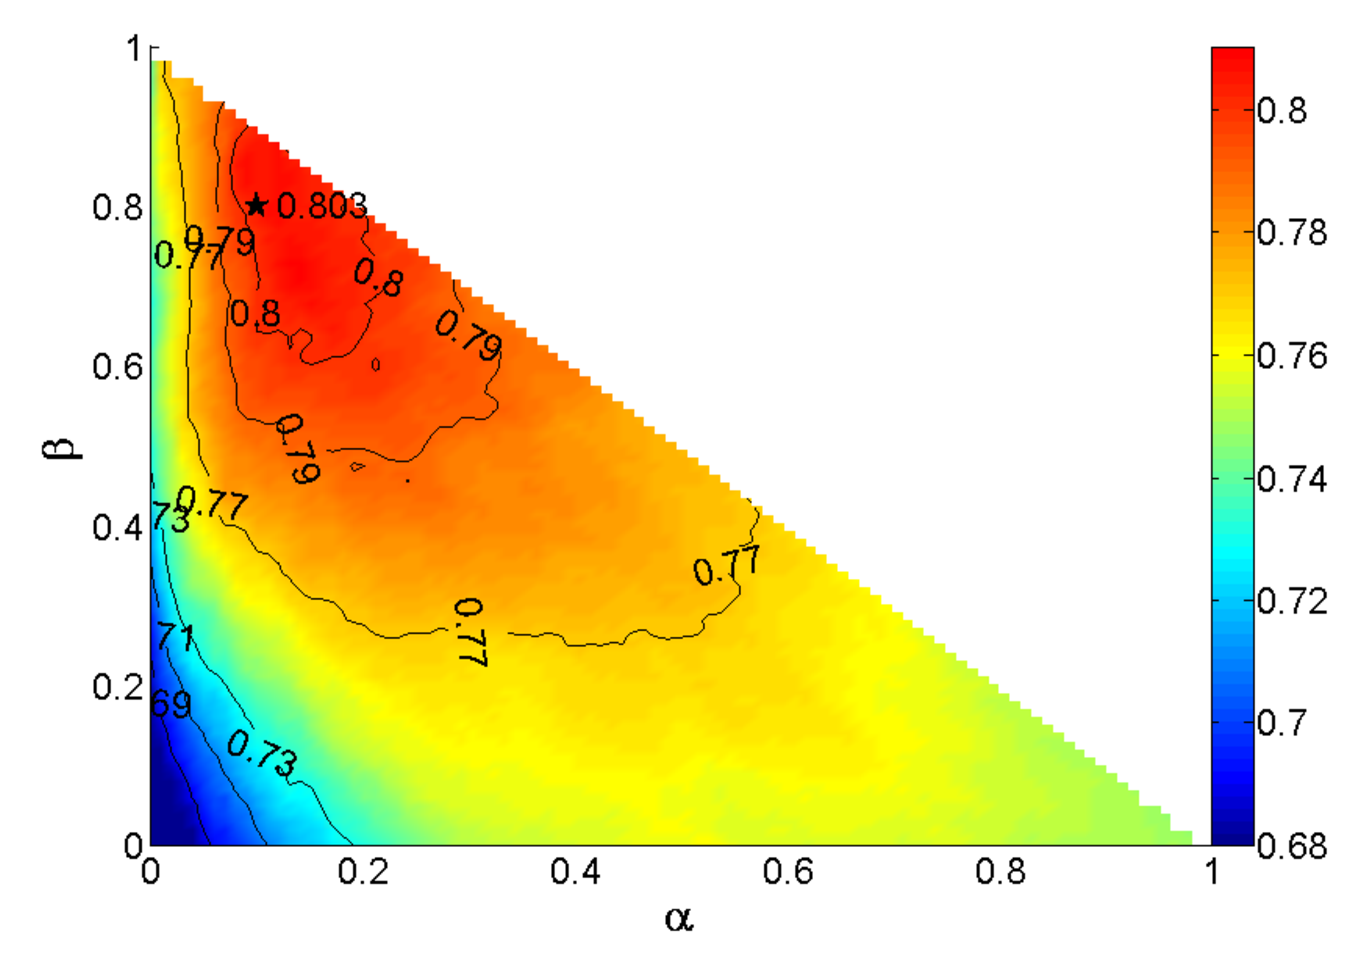
\includegraphics[scale=\graphscaleexpapp]{./exp/AAN-para-recm.eps}}
%\quad\quad
%\hspace{\graphmarginexpapp}
\hfill
\subfigure[{\scriptsize \aminer with \recom}]{\label{exp-aminer-ab-recom}
\includegraphics[scale=\graphscaleexpapp]{./exp/AMiner-para-recm.eps}}
%\quad\quad
%\hspace{\graphmarginexpapp}
\hfill
\subfigure[{\scriptsize \magdata with \recom}]{\label{exp-mag-ab-recom}
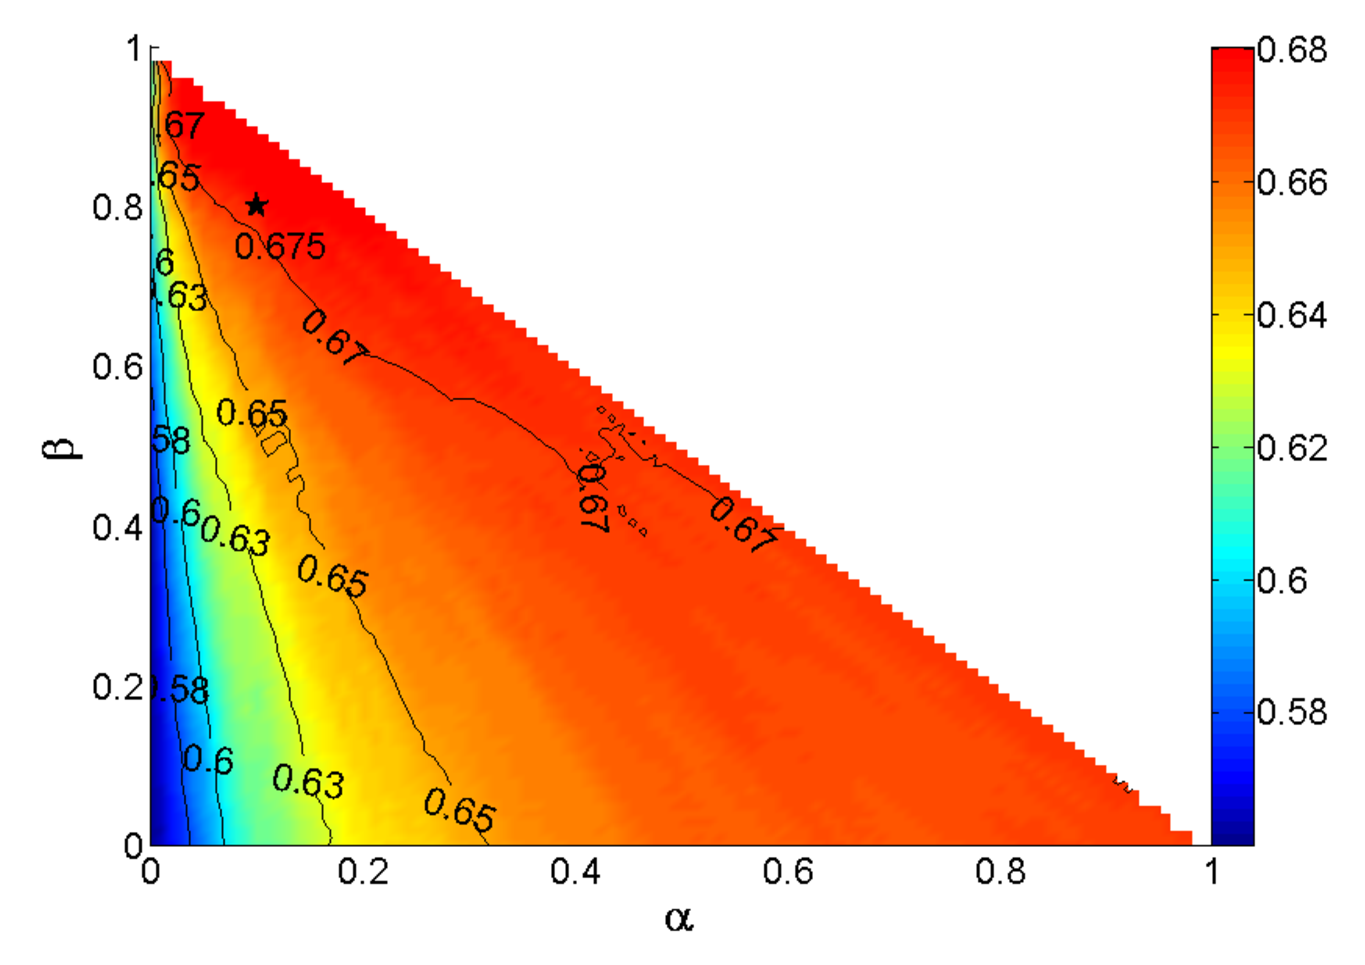
\includegraphics[scale=\graphscaleexpapp]{./exp/MAG-para-recm.eps}}
\\ %%%%%%%%%%%%%%%%%%%%%%%%%%%%%%%%%%%%%%
\vspace{-2ex}
%\hspace{-10ex}
\subfigure[{\scriptsize \aan  with \fcita}]{\label{exp-aan-ab-fcita}
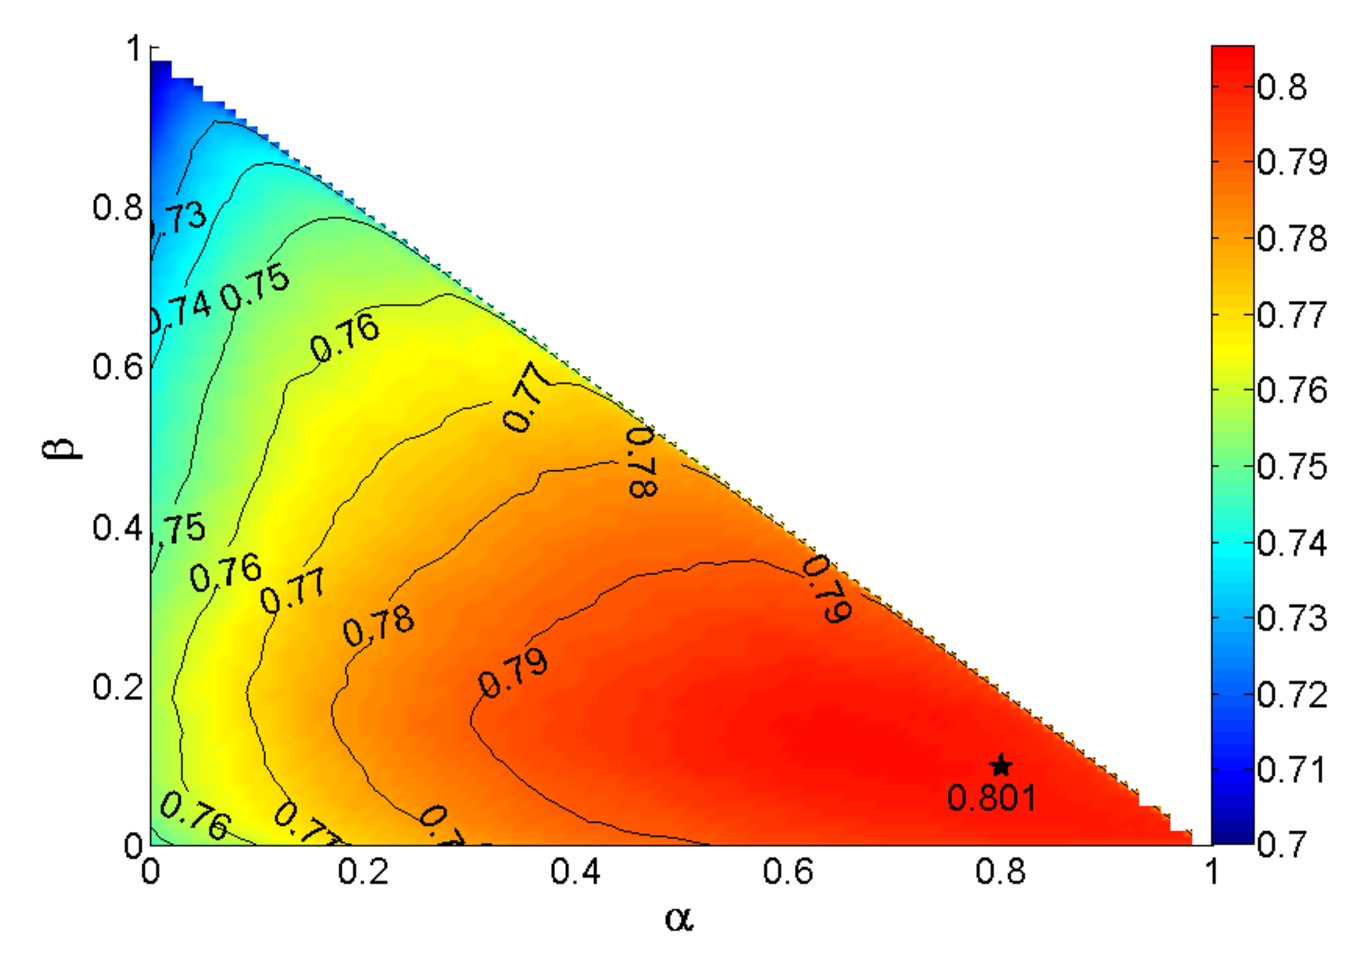
\includegraphics[scale=\graphscaleexpapp]{./exp/AAN-para-fcita.eps}}
%\quad\quad
%\hspace{\graphmarginexpapp}
\hfill
\subfigure[{\scriptsize \aminer with \fcita}]{\label{exp-aminer-ab-fcita}
\includegraphics[scale=\graphscaleexpapp]{./exp/AMiner-para-fcita.eps}}
%\quad\quad
%\hspace{\graphmarginexpapp}
\hfill
\subfigure[{\scriptsize \magdata with \fcita}]{\label{exp-mag-ab-fcita}
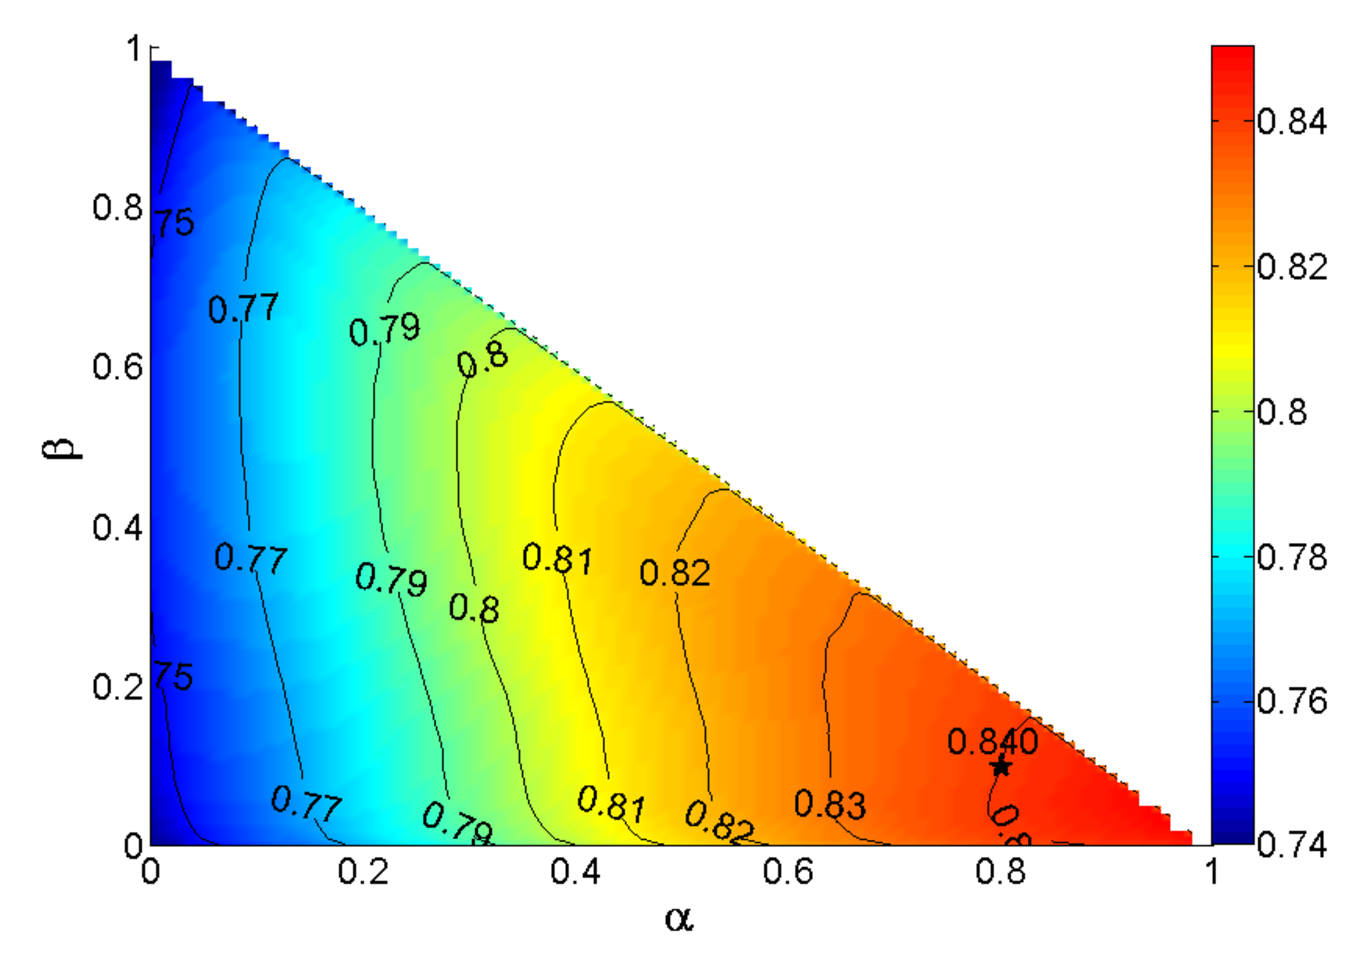
\includegraphics[scale=\graphscaleexpapp]{./exp/MAG-para-fcita.eps}}
\end{center}
\vspace{-2.5ex}
\caption{\small Accuracy tests: varying aggregating parameters $\alpha$ and $\beta$}
\label{exp-ab}
\vspace{-3ex}
\end{figure*}
%%%%%%%%%%%%%%%%%%%%%%%%%%%%%%%%%%%%%%

\stitle{Exp-4: Impacts of parameters}.
%\subsubsection{Exp-4: Impacts of parameters}.
In the last set of tests, we evaluated the impacts of time decaying factor $\sigma$, importance weighting factor $\lambda$, aggregating parameters $\alpha$ and $\beta$, and the TWPageRank. We fixed these parameters as well as $Y_s$ to their default values, used the TWPageRank proposed in this work by default, and tested the \PairAcc with the entire \recom and \fcita (\ie $T_i=+\infty$, $dif=1$).

%We present main results only and more details are available in~\cite{SARank-full}.




\etitle{Exp-4.1}.
%\stitle{Exp-4.1}.
To evaluate the impacts of the time decaying factor $\sigma$, we varied $\sigma$ from -1.6 to -0.4.
%, while fixed $Y_s$ to default values, $T_i=+\infty$, $dif=1$ and $\lambda=0.5$.
The results of \PairAcc are reported in Figs.~\ref{exp-aan-sigma}, \ref{exp-aminer-sigma} and \ref{exp-mag-sigma}.
%with both sets of ground-truth


When varying $\sigma$, the \PairAcc of \ensemblerank is very stable on all datasets using both \recom and \fcita. Indeed, with \recom and \fcita, the \PairAcc only varies (0.42\%, 1.55\%, 0.81\%) and (1.26\%, 0.96\%, 1.16\%) on (\aan, \aminer, \magdata), respectively.
%
%We omitted the detailed results of running time due to space constraint.
The running time varies (11.3\%, 8.6\%) on average only on (\aminer, \magdata), respectively.
%(0.18, 33.6) seconds, \ie

%Both of these show the robustness of \ensemblerank to the time decaying factor $\sigma$.

%As we can see from the figure, our method \ensemblerank is almost stable with the reduction of $\sigma$, since there is only a small fluctuation and the accuracy of our methods is always higher than the best baseline result in all datasets regardless of the change of $\sigma$. This means \ensemblerank is insensitive with $\sigma$.


%%%%%%%%%%%%%%%%%%%%%%%%%%%%%%%%%%%%%%%%%%%%%%%%%%
\begin{table}[tb!]
%\vspace{-2ex}
\begin{center}
\caption{\small Accuracy tests using different components with \recom (rows 2--4) and \fcita (rows 5--7).}
\label{tab-recom}
\begin{small}
\vspace{-.5ex}
\begin{tabular}{|c| c |c | c|}
\hline
{\bf Datasets} & {\bf C}\hspace{5ex}{\bf V}\hspace{5ex}{\bf A} & {\bf CV}\hspace{3ex}{\bf CA}\hspace{3ex}{\bf VA} & {\bf CVA} \\
\hline \hline
% \recom
\aan & 0.752 \ 0.616 \ 0.649 & 0.809 \ 0.764 \ 0.747 & {\bf 0.810} \\
\aminer & 0.735 \  0.581 \  0.640 & 0.784 \ 0.749 \ 0.729 & {\bf 0.785} \\
\magdata & 0.635 \ 0.534 \ 0.553 & 0.697 \ 0.673 \  0.648 & {\bf 0.698} \\ \hline
% \ficta
\aan & 0.785 \ 0.557 \ 0.761 & 0.849 \ 0.866 \ 0.771 & {\bf 0.870} \\
\aminer & 0.713 \  0.603 \  0.725 & 0.843 \ 0.847 \ 0.740 & {\bf 0.856} \\
\magdata & 0.736 \ 0.628 \ 0.718 & 0.848 \ 0.857 \ 0.751 & {\bf 0.874} \\
\hline
\end{tabular}
\end{small}
\end{center}
\vspace{-6ex}
\end{table}
%%%%%%%%%%%%%%%%%%%


\etitle{Exp-4.2}.
%\stitle{Exp-4.2}.
To evaluate the impacts of importance weighting factor $\lambda$, we varied $\lambda$ from 0 to 1.
%while fixed $Y_s$ to default values, $T_i=+\infty$, $dif=1$ and $\sigma=-1.0$.
The results of \PairAcc are reported in Figs.~\ref{exp-aan-lambda}, \ref{exp-aminer-lambda} and \ref{exp-mag-lambda}. Note that parameter $\lambda$ has no impacts on efficiency.
%with both sets of ground-truth

When varying $\lambda$, the \PairAcc of \ensemblerank first increases and then decreases on all datasets with both \fcita and \recom, except on \aminer with \recom.
%\marked{The value of $\lambda$ for \ensemblerank to achieve the best effectiveness is (0.6, 0, 0.2) and (0.6, 0.4, 0.1) on (\aan, \aminer, \magdata) with \recom and \fcita, respectively.}
This result indicates that combining prestige and popularity generally produces more robust results than using either of prestige and popularity.
Indeed, with \recom and \fcita, the \PairAcc of combining prestige and popularity is (10.2\%, 10.7\%, 5.5\%) and (8.0\%, 8.7\%, 9.0\%) higher than using prestige alone, and is (1.2\%, -0.1\%, 1.0\%) and (1.0\%, 1.0\%, 0.3\%) higher than using popularity alone on (\aan, \aminer, \magdata), respectively.


%The selection of $\lambda$ is influenced by ground-truth, such that the best $\lambda$ falls into $[xx,xx]$ and $[yy,yy]$ on \fcita and \recom, respectively. Moreover, equally weighting, \ie $\lambda=0.5$, is a good default setting when no query information is available in advance.
%Indeed, the best obtained \PairAcc using (\fcita, \recom) is only (0.10\%, 0.38\%), (0.04\%, 2.59\%) and (0.06\%, 0.91\%)  higher than the \PairAcc of equally weighting on \aan, \aminer and \magdata, respectively.





\etitle{Exp-4.3}.
To evaluate the impacts of aggregating parameters $\alpha$ and $\beta$, we varied $\alpha$ and $\beta$ at the granularity of 0.01. Again, parameters $\alpha$ and $\beta$ have few impacts on efficiency. The results are reported in Fig.~\ref{exp-ab}, where the parameters selected earlier and their corresponding \PairAcc are marked with $*$.

When varying $\alpha$ and $\beta$, the \PairAcc of \ensemblerank changes gently, as shown in Fig.~\ref{exp-ab}.
The optimal \PairAcc is obtained within a single region, rather than a complex collection of optimal regions.
%
Moreover, the \PairAcc keeps at a high level within a certain ($\alpha$, $\beta$) combination space around the optimal region, as shown in Fig.~\ref{exp-ab}.
%For instance, consider a square of length 0.3, which covers 8.5\% of the parameter combination space. The fraction of parameters such that the \PairAcc is no worse than 1\% of the corresponding \PairAcc with marker $*$ is (73\%, 94\%) on \aan, (96\%, 87\%) on \aminer and (83\%, 95\%) on \magdata, using (\recom, \fcita), respectively.
%
Further, the optimal parameters on the same sets of ground-truth are very similar for (\aan, \aminer and \magdata), indicating that the setting of $\alpha$ and $\beta$ can be easily transferred across different datasets.
To conclude, \ensemblerank is very robust to parameters $\alpha$ and $\beta$, and it is quite flexible for choosing proper values of parameters $\alpha$ and $\beta$.

Moreover, this enables to verify the effectiveness of importance assembling from different components, whose results are reported in Table~IV, in which letters C, V and A stand for citation, venue and author components, respectively.
The ranking based on all components consistently performs the best, using both \recom and \fcita, which justifies the use of importance assembling for ranking scholarly articles.
%which, using \recom and \fcita, improves the \PairAcc over using components (C, V, A, CV, CA, VA) by (5.77\%, 19.4\%, 16.1\%, 0.09\%, 4.59\%, 6.28\%) and (9.54\%, 23.7\%, 5.90\%, 2.50\%, 0.71\%, 4.79\%) on \aan, (6.94\%, 23.7\%, 14.4\%, 0.21\%, 1.56\%, 7.67\%) and (17.68\%, 12.4\%, 9.61\%, 0.33\%, 1.88\%, 6.34\%) on \aminer, and (6.29\%, 16.38\%, 14.45\%, 0.05\%, 2.43\%, 5.02\%) and (11.43\%, 19.2\%, 11.2\%, 1.44\%, 0.77\%, 9.62\%) on \magdata, respectively.


\eat{
\etitle{Exp-4.3}.
%\stitle{Exp-4.3}.
To evaluate the impacts of aggregating parameters $\alpha$ and $\beta$, we varied $\alpha$ and $\beta$ at the granularity of 0.01.
%while fixed $Y_s$ to default values, $T_i=+\infty$, $dif=1$, $\sigma=-1.0$ and $\lambda=0.5$.
Again, parameters $\alpha$ and $\beta$ have few impacts on efficiency. Due to space limitations, we only present the main results and more details are available at~\cite{SARank-full}.

Indeed, \ensemblerank is very robust to parameters $\alpha$ and $\beta$.
(a) When varying $\alpha$ and $\beta$, the \PairAcc of \ensemblerank changes gently. (b) \PairAcc also keeps at a high level within a certain ($\alpha$, $\beta$)  combination space. Finally, (c) the optimal parameters on the same set of ground-truth are very similar for \aan, \aminer and \magdata. That is, it is quite flexible for choosing proper values
of  parameters $\alpha$ and $\beta$.
} %%%%%%%% brief version of Exp-4.3

%%%%%%%%%%%%%%%%%%%%%%%%%%%%%%%%%%%%%%
\begin{figure*}[tb!]
%\vspace{1ex}
\addtolength{\subfigcapskip}{-1ex}
\begin{center}
\subfigure[{\scriptsize \aan with \recom}]{\label{exp-aan-recom-drank}
\includegraphics[scale=0.35]{./exp/AAN_TWPageRank_recom.eps}}
\hfill
%\hspace{\graphmarginexpapp}
\subfigure[{\scriptsize \aminer with \recom}]{\label{exp-aminer-recom-drank}
\includegraphics[scale=0.35]{./exp/AMiner_TWPageRank_recom.eps}}
\hfill
%\hspace{\graphmarginexpapp}
\subfigure[{\scriptsize \magdata with \recom}]{\label{exp-mag-recom-drank}
\includegraphics[scale=0.35]{./exp/MAG_TWPageRank_recom.eps}}
\\%%%%%%%%%%%%%%%%%%%%%%%%%%%%%%%%%%%%%%%%%%%
\vspace{-1.5ex}
\subfigure[{\scriptsize \aan with \fcita}]{\label{exp-aan-fcita-drank}
\includegraphics[scale=0.35]{./exp/AAN_TWPageRank_fcita.eps}}
\hfill
%\hspace{\graphmarginexpapp}
\subfigure[{\scriptsize \aminer with \fcita}]{\label{exp-aminer-fcita-drank}
\includegraphics[scale=0.35]{./exp/AMiner_TWPageRank_fcita.eps}}
\hfill
%\hspace{\graphmarginexpapp}
\subfigure[{\scriptsize \magdata with \fcita}]{\label{exp-mag-fcita-drank}
\includegraphics[scale=0.35]{./exp/MAG_TWPageRank_fcita.eps}}
\end{center}
\vspace{-2.5ex}
\caption{\small Impacts of the TWPageRank on accuracy: varying importance weighting
factor $\lambda$}
\label{exp-drank}
\vspace{-3ex}
\end{figure*}
%%%%%%%%%%%%%%%%%%%%%%%%%%%%%%%%%%

\newcommand{\drank}{\kw{DRank}}


\etitle{Exp-4.4}.
\marked{To evaluate the impacts of the proposed TWPageRank, we compared our approach \ensemblerank with an algorithm alternative (referred to as \drank) the same to \ensemblerank except exploiting exponentially decayed impact weights, \ie $w(u,v)=e^{\sigma(T_u-T_v)}$ in Eq.~(\ref{eq-infl-weights}).
%The two algorithms produce the same popularity while different prestige.
To better understand the impacts, we varied the importance weighting factor $\lambda$ from 0.1 to 1. Note that the ranking results are the same when $\lambda=0$ due to the same popularity computation. The results are reported in Fig.~\ref{exp-drank}, where the numbers represent the improvement of \PairAcc by \ensemblerank over the one by \drank.}

\marked{
When varying $\lambda$, the \PairAcc of \ensemblerank is better than the one of \drank in most cases, which shows the superiority of the TWPageRank than exploiting exponentially decayed weights.
The difference of \PairAcc by the two algorithms is higher with \recom than with \fcita, since the two algorithms are using citation information to predict past and future citations with \fcita.
Moreover, algorithm \ensemblerank is consistently better than \drank when $0.5 \le \lambda \le 0.9$.
%, which, with \recom and \fcita, improves the \PairAcc by (2.88\%, 3.91\%, 3.90\%) and (0.55\%, 0.50\%, 0.22\%) on (\aan, \aminer, \magdata) on average, respectively.
The improvement decreases with the decrease of $\lambda$ as the popularity dominates the ranking with small $\lambda$, and in some cases, \drank outperforms \ensemblerank. %as the prestige and popularity orders of article pairs are more diverse for \drank than \ensemblerank.
Overall, with \recom and \fcita, \ensemblerank improves the \PairAcc over \drank by (1.78\%, 3.07\%, 3.20\%) and (0.29\%, 0.48\%, 0.11\%) on (\aan, \aminer, \magdata) on average, respectively.
}

\marked{
The TWPageRank has little impacts on efficiency, and the running time of the two algorithms only varies (6.34\%, 4.83\%) on (\aminer, \magdata) on average, respectively.}

\eat{
With the increment of $\lambda$, \ensemblerank has more promotion than DRank and the \PairAcc of DRank is better than \ensemblerank with small $\lambda$, possibly due to the addition of popularity will correct the mistaken pairs better on DRank, although \ensemblerank rank more pairs correctly.
In addition, the change of \PairAcc with \recom is higher than the one with \fcita, possibly due to the article pairs in \fcita are of the same years.
Moreover, the \PairAcc of \ensemblerank is better than its counterparts from $\lambda=0.5$ to $\lambda=1$, except on \aminer with \fcita. Recall that in Fig.~\ref{exp-aminer-lambda} using popularity alone gives the best results on \aminer, indicating that the prestige computed by TWPageRank is less accurate on \aminer than on the other two datasets.
%
Indeed, with \recom and \fcita, the \PairAcc of \ensemblerank is (2.20\%, 6.63\%, 5.68\%) and (0.25\%, 0.05\%, 0.05\%) higher than DRank on (\aan, \aminer, \magdata), respectively, when using prestige alone, and is (1.73\%, 2.97\%, 2.92\%) and (0.22\%, -0.08\%, 0.17\%) higher when combining prestige and popularity, respectively, on average.
%
Finally, the TWPageRank has little impacts on efficiency, and the running time of \ensemblerank and its counterparts only changes (6.34\%, 4.83\%) on (\aminer, \magdata) on average, respectively.
}

\stitle{Summary}.
From these tests we find the followings.


\sstab(1) Our model \ensemblerank is effective for ranking scholarly articles, which is consistently better than competitive methods in all tests. With \recom and \fcita, \ensemblerank improves \PairAcc over (\pagerank, \futurerank, \hhgrank) by
(13.5\%, 6.8\%, 4.8\%) and (12.0\%, 3.0\%, 3.2\%) on \aan,
(12.7\%, 5.0\%, 4.9\%) and (14.0\%, 6.5\%, 4.6\%) on \aminer, and
(6.5\%, 2.5\%, 2.2\%) and (13.4\%, 6.0\%, 2.4\%) on \magdata, on average, respectively.
%, and it has a great advantage in evaluating the importance in a long term. Furthermore, it is more accurate evaluating articles which have just published and is in lack of citations, since it uses both venue network and author information besides of citation network. Indeed, it improves the accuracy by $(7.9\%, 3.2\%, 2.3\%)$ and $(14.4\%, 5.0\%, 3.8\%)$ over \pagerank, \futurerank and \hhgrank on average of three datasets with recommendation based ground truth and future citation ground truth, respectively.


\sstab(2) Our batch algorithm \batensemble and incremental algorithm \incensemble are also efficient.
%
Our incremental algorithm \incensemble is on average (1.7, 3.1, 2.8, 117) and (2.0, 3.0, 4.4, 245) times faster than (\batensemble, \powensemble, \futurerank, \hhgrank)  on the large \aminer and \magdata, respectively.

%The batch algorithm \batensemble is on average (1.3, 2.5, 348) times faster than (\powensemble, \futurerank, \hhgrank)  on the largest \magdata, respectively.

%\noindent (3) Our incremental algorithms are much faster than their batch counterparts in practice, even their time complexity is very close. Indeed, algorithms \inctwprdag, \inctwprscc and \incensemble further improve the efficiency of (\twprdag, \twprscc, \batensemble) by (23\%, 38\%, 22\%) on average, respectively.


\sstab(3) Our ranking model \ensemblerank introduces the time decaying factor $\sigma$, importance weighting factor $\lambda$ and aggregating parameters $\alpha$ and $\beta$ for the sake of practicability and flexibility in real-life applications, and, from our tests, \ensemblerank is very robust to these parameters. Moreover, the proposed TWPageRank is generally more effective than directly using exponentially decayed impact weights.




% \stitle{Related work}. We summarize related work as follows.
%
%Scholarly article ranking

Scholarly article ranking has shifted from citation count analysis~\cite{Garfield471,Hirsch15112005} to graph analysis~\cite{ChenXMR07,Zhou07-CoRank,Jiang12-MRank,Liang16AAAI,Li08TSRanking,Wang13AAAI,WalkerXKM07,sayyadi09,
Wang16TIST,Ng11KDD}.
Based on the information used, these methods are divided into four categories: (a) using the citation information only~\cite{Garfield471,Hirsch15112005,ChenXMR07,Ng11KDD}, (b) using the citation and temporal information~\cite{Li08TSRanking,WalkerXKM07}, (c) using the citation information and other heterogeneous information, \eg authors and venues of articles~\cite{Zhou07-CoRank,Jiang12-MRank,Liang16AAAI}, and (d) combining the citation, temporal and other heterogeneous information~\cite{sayyadi09,Wang16TIST,Wang13AAAI}.
Our work belongs to the last category aiming at fully employing information available for scholarly article ranking.


%\stitle{PageRank\&weighted PageRank algorithms}.

%PageRank \cite{Brin98:PageRank} and its extensions have been extensively used for citation analyses \cite{Waltman2014}. While PageRank equally propagates scores along outlinks, Weighted PageRank \cite{Xing04:WPR} extends PageRank by distributing scores based on the popularity of pages. Different from previous work, the Time-Weighted PageRank proposed in this work discriminately propagates scores in terms of citation statistics.

PageRank \cite{Brin98:PageRank} and its extensions have been extensively used for citation analyses \cite{Waltman2014}. While PageRank equally propagates scores along outlinks, Weighted PageRank extends PageRank by distributing scores based on certain criteria such as popularity of pages~\cite{Xing04:WPR} or authority of authors~\cite{Ding11}. Different from previous work, the Time-Weighted PageRank proposed in this work discriminately propagates scores in terms of citation statistics.






%\stitle{Dynamic algorithms}.

Dynamic algorithms have proven useful for various tasks by avoiding computing from scratch~\cite{RamalingamR93}.
% and only recomputing those affected by updates
%Dynamic algorithms have proven useful for graph analysis tasks, \eg incremental graph pattern matching~\cite{FanWW13} and  incremental simrank computation~\cite{YuLZ14}.
To our knowledge, little concern has been paid to dynamic scholarly article ranking except that~\cite{GhoshKHLL11} uses PageRank in dynamic citation networks. However, its solution is based on a strong and impractical assumption that there are no citations between articles in the same years.
Further, although there exist several studies on incremental PageRank computation~\cite{DesikanPSK05,AbiteboulPC03,WuR09} and on incremental PageRank approximation \cite{BahmaniCG10,BahmaniKMU12}, they are not designed for scholarly article ranking.
%
Different from previous work, we study scholarly article ranking in a dynamic environment in terms of
the citation characteristics of scholarly articles, which has never been exploited before.

%Our approach only makes the assumption that there are no mutual references within the citation network, which, we admit, violates xx\% of total citations on \magdata, and is significantly different (yy\% on \magdata) from~\cite{GhoshKHLL11}.  - move to Section 3

Ensemble methods use multiple learners to obtain better performance than could be obtained from a constituent learner alone~\cite{zhihua-book}.
%In this work, we leverage ensembles to produce better and robust results for scholarly article ranking~\cite{zhihua-book,wsdmcup,DuanAMHH16}.
In this work, we leverage  importance assembling  to produce better and robust results for scholarly article ranking~\cite{zhihua-book,wsdmcup,DuanAMHH16}.

%\balance
\vspace{-1ex}
%%%%%%%%%%%%%%%%%%%%%%%%%%%%%%%%%%%%%%%%%%%%%%%%%%%%%%%%%%%%%%%%%%%%%%%%%%%%%%
\section{Conclusions}
%%%%%%%%%%%%%%%%%%%%%%%%%%%%%%%%%%%%%%%%%%%%%%%%%%%%%%%%%%%%%%%%%%%%%%%%%%%%%%

We have evaluated the state-of-the-art \lsa algorithms for trajectory compression, including \emph{both the optimal and the sub-optimal methods that use either \ped or \sed}. 
Using a variety of real trajectory datasets, we evaluated the performance of each technique.% in terms of its processing time, compression ratio and average error.
Our experimental results show that 
(1) the output sizes of algorithms using \sed are approximate $2$ times of using \ped, 
(2) the output sizes of sub-optimal algorithms are $130\%$--$160\%$ of the optimal algorithms, and 
(3) the one-pass algorithms \siped and \operb and \cised are tens of times faster than the batch algorithms and \textcolor{red}{$xxx$} times faster than online algorithms, while they still have comparable compression ratios with batch algorithms. Hence, they are more suitable for resource constraint mobile devices.

%\balance
\input{sec-appendix-related}
%

\section*{Appendix: Examples}


\begin{example}
	\label{exm-notations}
	Consider Figure~\ref{fig:notations}, in which
	%
	(1) $\dddot{\mathcal{T}}[P_0$, $\ldots, P_{10}]$ is a trajectory having 11 data points,
	%
    (2) the set of two continuous line segments $\{\vv{P_0P_4}$, $\vv{P_4P_{10}}$\}, the set of four continuous line segments $\{\vv{P_0P_2}$, $\vv{P_2P_4}$, $\vv{P_4P_7}$, $\vv{P_7P_{10}}$\} and the set of three continuous line segments $\{\vv{P_0P_4}$, $\vv{P_4P_5}$, $\vv{P_5P_{10}}$\} are three piecewise line representations of trajectory $\dddot{\mathcal{T}}$,
	%
	(3) $ped(P_4, \vv{P_0P_{10}})=|\vv{P_4P^*_4}|$, where $P^*_4$ is the perpendicular point of $P_4$ \wrt line segment $\vv{P_0P_{10}}$,
	%
	(4) For $P_4$, its synchronized point $P'_4$ \wrt $\vv{P_0P_{10}}$ satisfies $\frac{|\vv{P_0P'_4}|}{|\vv{P_0P_{10}}|} = \frac{P_4.t - P_0.t}{P_{10}.t-P_0.t} = \frac{4-0}{10-0}= \frac{2}{5}$,
	%
	(5) $sed(P_4, \vv{P_0P_{10}})= |\vv{P_4P'_4}|$, $sed(P_2, \vv{P_0P_{4}})= |\vv{P_2P'_2}|$ and $sed(P_7, \vv{P_4P_{10}})$ $=$ $|\vv{P_7P'_7}|$,
	where points $P'_4$, $P'_2$ and $P'_7$ are the synchronized points of $P_4$, $P_2$ and $P_7$ \wrt line segments $\vv{P_0P_{10}}$, $\vv{P_0P_{4}}$ and $\vv{P_4P_{10}}$, respectively.  and
    %
    (6) $dad(\vv{P_5P_6}, \vv{P_0P_{10}})=\theta_{56}$ is the \dad of line segment $\vv{P_5P_6}$ to $\vv{P_0P_{10}}$.
\end{example}








\begin{example}
\label{exm-alg-lsa}
Consider the trajectory $\dddot{\mathcal{T}}[P_0,\ldots,P_{10}]$ shown in Figure~\ref{fig:notations}.
The $\dpa$ Algorithm firstly creates $\vv{P_0P_{10}}$, then it calculates the distance of each point in $\{P_0,\ldots,P_{10}\}$ to $\vv{P_0P_{10}}$.
It finds that $P_{4}$ has the maximum distance to $\vv{P_0P_{10}}$, which is greater than $\epsilon$. Then it goes to compress sub-trajectories $[P_0, \ldots, P_{4}]$ and $[P_{4}, \ldots, P_{10}]$, separately.
When using \sed (right), the sub-trajectory $[P_4,\ldots, P_{10}]$ is further split to $[P_4$, $\ldots$, $P_7]$ and $[P_7$, $P_{10}]$.
Finally, the algorithm outputs two continuous directed line segments $\vv{P_0P_4}$ and $\vv{P_4P_{10}}$ when using \ped, and three continuous directed line segments $\vv{P_0P_4}$, $\vv{P_4P_7}$ and $\vv{P_7P_{10}}$ when using \sed.
\end{example}



\begin{example}
\label{exm-alg-pavlidis}
Figure~\ref{fig:pavlidis} is an example of the \tpa algorithm.

\ni (1) Initially, $10$ line segments are created, and for each pair of adjacent segments, the costs of merging them are calculated and saved. For example, the cost of merging $\vv{P_0P_1}$ and $\vv{P_1P_2}$ is $ped(P_{1}, \vv{P_0P_{2}}) = 0.32\epsilon$.
%
(2) The cost of merging $\vv{P_6P_7}$ and $\vv{P_7P_8}$ is $0.02\epsilon$, which is the minimal value among all costs. Hence, $\vv{P_6P_7}$ and $\vv{P_7P_8}$ are merged to $\vv{P_6P_8}$. The cost of merging $\vv{P_5P_6}$ and $\vv{P_6P_8}$, and the cost of merging $\vv{P_6P_8}$ and $\vv{P_8P_9}$ are further updated to $0.37\epsilon$ and $0.11\epsilon$, respectively.
%
(3) $\vv{P_2P_3}$ and $\vv{P_3P_4}$ are merged to $\vv{P_2P_4}$. The cost merging $\vv{P_2P_4}$ and $\vv{P_4P_5}$, and the cost of merging $\vv{P_1P_2}$ and $\vv{P_2P_4}$ are also updated.
%
(4) At last, the algorithm outputs two line segments $\vv{P_0P_4}$ and $\vv{P_4P_{10}}$.
\end{example}




\begin{example}
	\label{exm-alg-optimal}
	Figure~\ref{fig:optimal} is an example of the \opt algorithm using \ped taking as input the trajectory \trajec{T} shown in Figure~\ref{fig:notations}. The reachability graph of \trajec{T} is constructed and a shortest path with 2 edges is founded.
	At last, the algorithm outputs two line segments $\vv{P_0P_4}$ and $\vv{P_4P_{10}}$.	
\end{example}
\vspace{-1ex}

\begin{figure}[tb!]
	\centering
	\includegraphics[scale=0.75]{Figures/Fig-Optimal.png}\vspace{-2ex}
	\caption{\small Example of reachability graph of trajectory \trajec{T}$[P_0, \ldots, P_n]$ whose shortest path is $(P_0, P_4, P_{10})$.}	\vspace{-3ex}
	\label{fig:optimal}
\end{figure}




\begin{figure*}[tb!]
	\centering
	\includegraphics[scale=0.55]{Figures/Fig-Squishe.png}
	\vspace{-3ex}
	\caption{\small The trajectory $\dddot{\mathcal{T}}[P_0, \ldots, P_{10}]$ is compressed by the \squishe algorithm using \sed to five line segments. The size of Q is 6, and the data structure after point $P$ is a tuple $(pre, suc, mmprio, prio)$. }
	\vspace{-1ex}
	\label{fig:squishe}
\end{figure*}









\begin{example}
\label{exm-alg-squishe}
Figure~\ref{fig:squishe} is an example of \squishe.
%
(1) Initially, $|Q| = 6$ points are read to the list. The tuple $(pre, suc, mmprio, prio)$ for each point is initialized. For example, the tuple of $P_1$ is set to $(0, 2, 0, 0.42\epsilon)$, where $0.42\epsilon$ is the \sed from $P_1$ to $\vv{P_0P_2}$.
%
(2) The priority of $P_3$ has the minimal value, thus, it is removed from the list.
The $mnprio$ properties of $P_2$ and $P_4$ are updated to $max\{mnprio(pre(P_3)), prio(P_3)\}$ = $max\{mnprio(P_2), prio(P_3)\}$ = $max\{0, 0.39\epsilon\}$ = $0.39\epsilon$, and $max\{mnprio(P_4), ~prio(P_3)\}$ = $0.39\epsilon$, respectively.
Furthermore, the $prio$ property of $P_4$ is updated to $mnprio(suc(P_j)) + sed(suc(P_j),\vv{pre(P_{j})suc(suc(P_{j}))})$ = $mnprio(P_4) + sed(P_4,\vv{P_2P_5})$ = $0.39\epsilon + 2.50\epsilon$ = $2.89\epsilon$, and the $prio$ property of $P_2$ is updated to $mnprio(P_2) + sed(P_2,\vv{P_1P_4})$ = $0.39\epsilon + 2.12\epsilon$ = $2.51\epsilon$.
Then, $P_6$ is read, and the information of $P_5$ is updated.
%
(3) $P_5$ is removed and $P_7$ is read to the list.
%
(4) Finally, the algorithm outputs 5 line segments $\vv{P_0P_2},\vv{P_2P_4},\vv{P_4P_7},\vv{P_7P_9}$ and $\vv{P_9P_{10}}$.
\end{example}




\begin{example}
\label{exm-alg-bqs}
Figure~\ref{fig:bqs} is an example of \bqsa. The bounding box $c_1c_2c_3c_4$ and the two lines $\vv{P_sP_{h}} = \vv{P_0P_1}$ and $\vv{P_sP_{l}} = \vv{P_0P_2}$ form a convex hull $u_1u_2c_2l_2l_1c_4$. \bqsa computes the distances of $u_1,u_2,c_2,l_2,l_1$ and $c_4$ to line $\vv{P_0P_6}$ when $k=6$ or to line $\vv{P_0P_7}$ when $k=7$.
%
When $k=6$, all these distances to $\vv{P_0P_6}$  are less than $\epsilon$, hence \bqsa goes on to the next point (case 2); When $k=7$,
the max and min distances to $\vv{P_0P_7}$ are larger and less than $\epsilon$, respectively, and \bqsa needs to compress sub-trajectory $[P_0, \ldots, P_7]$ along the same line as \dpa (case 3).
\end{example}

\begin{figure}[tb!]
%\vspace{-1ex}
\centering
\includegraphics[scale = 0.66]{Figures/Fig-BQS.png}
\vspace{-1ex}
\caption{{\small Examples for algorithm \bqsa.}}
\label{fig:bqs}
\vspace{-2ex}
\end{figure}




\begin{example}
	\label{exm-alg-operb}
	Figure~\ref{fig:operb} is a running example of the \operb algorithm compressing the same trajectory $\dddot{\mathcal{T}}[P_0, \ldots, P_{10}]$.
	(1) It takes $P_0$ as the start point, reads $P_1$ and sets $\mathcal{L}_1$ = $\vv{P_0P_1}$.
	(2) It reads $P_2$. The distance from $P_2$ to $\mathcal{L}_1$ is less than the threshold, thus, it updates $\mathcal{L}_1$  to $\mathcal{L}_2$ by the fitting function $\mathbb{F}$.
	(3) It reads $P_3$ and $P_4$, and updates $\mathcal{L}_2$ to $\mathcal{L}_3$ and $\mathcal{L}_3$ to $\mathcal{L}_4$, respectively.
	(4) It reads $P_5$. The distance from $P_5$ to $\mathcal{L}_4$ is larger than the threshold, thus, it outputs $\vv{P_0P_4}$ and start the next section taking $P_4$ as the new start point.
	(5) The process continues until all points have been processed. At last, the algorithm outputs two continuous line segments $\vv{P_0P_4}$ and $\vv{P_4P_{10}}$.
\end{example}


\begin{figure}[tb!]
	\centering
	\includegraphics[scale=0.66]{Figures/Fig-OPER.png}
	\vspace{-3ex}
	\caption{\small The trajectory $\dddot{\mathcal{T}}[P_0, \ldots, P_{10}]$ is compressed by the \operb algorithm using \ped to two line segments.}
	\vspace{-1ex}
	\label{fig:operb}
\end{figure}




\begin{example}
	\label{exm-alg-sleeve}
	Figure~\ref{fig:sleeve} is a running example of algorithm \siped($\frac{\epsilon}{2}$) taking as input the same trajectory $\dddot{\mathcal{T}}[P_0, \ldots, P_{10}]$. At the beginning, $P_0$ is the first start point, and points $P_1$, $P_2$, $P_3$, etc., each has a narrow \emph{sector}.
	For example, the narrow \emph{sector} $\mathcal{S}$($P_0$, $P_{3}$, $\epsilon/2$) takes $P_0$ as the center point and $\vv{P_0P^u_{3}}$ and $\vv{P_0P^l_{3}}$ as the border lines.
	Because $\bigsqcap_{i=1}^{4}\mathcal{S}(P_0, P_{0+i}, \epsilon/2) \ne \{P_0\}$ and $\bigsqcap_{i=1}^{5}\mathcal{S}(P_0, P_{0+i}, \epsilon/2) = \{P_0\}$, $\vv{P_0P_4}$ is output and $P_4$ becomes the start point of the next section.
	At last, the algorithm outputs two continuous line segments $\vv{P_0P_4}$ and $\vv{P_4P_{10}}$.
\end{example}

\begin{figure}[tb!]
	\centering
	\includegraphics[scale=0.66]{Figures/Fig-sleeve.png}
	\vspace{-3ex}
	\caption{\small The trajectory $\dddot{\mathcal{T}}$ is compressed by the sector intersection algorithm using \ped to two line segments.}
	\vspace{-1ex}
	\label{fig:sleeve}
\end{figure}





%%%%%%%%%%%%%%% example of Algorithm CISED
\begin{figure}[tb!]
	\centering
	\includegraphics[scale=0.66]{Figures/Fig-Conest.png}
	\vspace{-2ex}
	\caption{\small A running example of the \cised algorithm. The points and the oblique circular cones are projected on an x-y space. }%The trajectory $\dddot{\mathcal{T}}[P_0, \ldots, P_{10}]$ is compressed into four line segments.
	\vspace{-1ex}
	\label{fig:exm-const}
\end{figure}
%%%%%%%%%%%%%%%%

\begin{example}
\label{exm-alg-conest}
	Figure~\ref{fig:exm-const} shows a running example of \cised($\frac{\epsilon}{2}$) for compressing the trajectory \trajec{T} in Figure~\ref{fig:notations}.
	For convenience, we project the points and the oblique circular cones on a x-y space.
%	
	(1) After initialization, the \cised algorithm reads point $P_1$ and builds a narrow \emph{oblique circular cone}~\cone{(P_0, \mathcal{O}(P_{1}, \epsilon/2))}, taking $P_0$ as its apex and \circle{(P_1, \epsilon/2)} as its base (green dash). The \emph{circular cone} is projected on the plane $P.t-P_1.t=0$, and the inscribe regular polygon $\mathcal{R}_1$ of the projection circle is returned. As $\mathcal{R}^*$ is empty, $\mathcal{R}^*$ is set to $\mathcal{R}_1$.
%	
	(2) The algorithm reads $P_2$ and builds \cone{(P_0, \mathcal{O}(P_{2}, \epsilon/2))} (red dash). The \emph{circular cone} is also projected on the plane $P.t-P_1.t=0$ and the inscribe regular polygon $\mathcal{R}_2$ of the projection circle is returned. As $\mathcal{R}^*=\mathcal{R}_1$ is not empty, $\mathcal{R}^*$ is set to the intersection of $\mathcal{R}_2$ and $\mathcal{R}^*$, which is $\mathcal{R}_1 \bigsqcap \mathcal{R}_2 \ne \emptyset$.
%	
	(3) For point $P_3$, the algorithm runs the same routine as $P_2$ until the intersection of $\mathcal{R}_3$ and $\mathcal{R}^*$ is $\emptyset$. Thus, a line segment $\vv{P_0P_2}$ is generated, and the process of a new line segment is started, taking $P_2$ as the new start point and $P.t-P_3.t=0$ as the new projection plane.
%	
	(4) At last, the algorithm outputs four continuous line segments, \ie $\{\vv{P_0P_2}$, $\vv{P_2P_4}$, $\vv{P_4P_{7}}$, $\vv{P_7P_{10}}\}$. %\eop
\end{example} 	
\vspace{-1ex}







\begin{example}
	\label{exm-alg-interval}
	Figure~\ref{fig:interval} is a running example of the \emph{interval} method taking as input the same trajectory $\dddot{\mathcal{T}}[P_0, \ldots, P_{10}]$. At the beginning, $P_0$ is the first start point, and points $P_1$, $P_2$, $P_3$, etc., each has a \emph{direction range} $Range(\vv{P_0P_1}, \epsilon)$, $Range(\vv{P_1P_2}, \epsilon)$, $Range(\vv{P_2P_3}, \epsilon)$, etc., respectively.
	%
	Because $\bigsqcap_{i=1}^{4}Range(\vv{P_{0+i-1}P_{0+i}}, \epsilon) \ne \phi$ and $\vv{P_0P_{4}}.\theta$ falls in the \emph{common subinterval}, and $\bigsqcap_{i=1}^{5}Range(\vv{P_{0+i-1}P_{0+i}}, \epsilon) = \phi$, $\vv{P_0P_4}$ is output and $P_4$ becomes the start point of the next section.
	At last, the algorithm outputs two continuous line segments $\vv{P_0P_4}$ and $\vv{P_4P_{10}}$.
\end{example}


\begin{figure}[tb!]
	\centering
	\includegraphics[scale=0.66]{Figures/Fig-interval.png}
	\vspace{-3ex}
	\caption{\small The trajectory $\dddot{\mathcal{T}}$ is compressed by the interval algorithm using \dad to two line segments.}
	\vspace{-1ex}
	\label{fig:interval}
\end{figure}










%\vspace{-1ex}
%\section*{Acknowledgments}
%This work is supported in part by NSFC (61925203 \& U1636210 \& 61421003) and  Beijing Advanced Innovation Center for Big Data and Brain Computing. For any correspondence, please refer to Shuai Ma.



%
% The following two commands are all you need in the
% initial runs of your .tex file to
% produce the bibliography for the citations in your paper.
\balance
\bibliographystyle{acm}
\begin{small}
\bibliography{sec-ref}
\end{small}




%\balancecolumns

\end{document}
